\PassOptionsToPackage{table,dvipsnames,svgnames}{xcolor}
\documentclass[%
  draft=false, % Set to 'false' before final printing
	a4paper,
  fontsize=11pt,
  version=last,
	BCOR=10mm,
	DIV=11,
	toc=bibliography,
	toc=listof,
	toc=index,
	hyperref,
	amsmath,
	ngerman,
	twoside,
	headinclude=true,
	footnotes=multiple,
	openany
 ]{scrbook}

\usepackage[TS1,T1]{fontenc}
\usepackage{libertine}
\usepackage{amsmath,amssymb,marvosym}
\usepackage{textcomp} % required to get special symbols
\usepackage[varqu,varl]{zi4}
\usepackage[libertine,cmintegrals,varbb,slantedGreek]{newtxmath}
\usepackage[scr=rsfso]{mathalfa}
\usepackage{bm}
%\useosf % Use old-style numbers in text but not in math mode. N.b: Avoid old-style figures in the pagination.
\usepackage[utf8]{inputenc}


\usepackage{icomma}
\usepackage{superiors}
\usepackage{fnpct}
\usepackage[final]{microtype}

\usepackage[ngerman,american]{babel}
\AtBeginDocument{\selectlanguage{american}}
\newcommand*{\ngerman}[1]{\foreignlanguage{ngerman}{#1}}
\newcommand*{\usenglish}[1]{\foreignlanguage{american}{#1}}

\usepackage[autostyle,german=quotes,english=american]{csquotes}

\usepackage{setspace}
\setstretch{1.2}

\usepackage[headsepline,plainheadsepline]{scrlayer-scrpage}
\pagestyle{scrheadings}
\ohead[\pagemark]{\pagemark}
\chead[]{}
\ihead[]{\headmark}
\ifoot[]{}
\cfoot[]{}
\ofoot[]{}
\setkomafont{pageheadfoot}{\normalfont\sffamily}
\setkomafont{pagenumber}{\sffamily\bfseries}
\setkomafont{descriptionlabel}{\normalfont\slshape}
\deffootnote[2em]{2.5em}{1.5em}{\thefootnotemark\ }

\KOMAoptions{DIV=last}


\usepackage[final]{graphicx}
\usepackage[table,dvipsnames,svgnames]{xcolor}
\usepackage{KAcolors}

\usepackage{tikz}
\usetikzlibrary{positioning,matrix,graphs,arrows,patterns,shapes,external,calc,fit,backgrounds,shadows,trees}
\usepackage{pgfplots}
\usepgfplotslibrary{ternary}
\tikzsetexternalprefix{./figures-compiled/}
\tikzset{external/aux in dpth={false},external/disable dependency files}
\tikzexternalize[shell escape=-enable-write18]

\tikzset{
  /tikz/line width=0.6pt,%  Default line width is 'semithick'
}

\pgfplotsset{
  compat=1.11,%
  plot coordinates/math parser=false,%
  tick label style={font=\footnotesize},%
  label style={font=\small},%
	scale only axis,%
	axis lines=center,%
	axis on top,%
  every axis legend/.append style={cells={anchor=west},draw=none,font=\small},%
  every axis plot/.append style={semithick},%
	KIT scatter plot A/.style={%
    draw=none,only marks,mark=*,mark options={draw=KITblue,fill=KITblue}},%
	KIT scatter plot B/.style={%
    draw=none,only marks,mark=square*,mark options={draw=KITred,fill=KITred}},%
	KIT scatter plot C/.style={%
    draw=none,only marks,mark=diamond*,mark options={draw=KITorange,fill=KITorange}},%
	KIT scatter plot explicit/.style={%
    scatter,%
    scatter/classes={%
      a={mark=*,KITblue},%
      b={mark=square*,KITred},%
      c={mark=diamond*,KITorange}},%
    only marks,%
    scatter src=explicit symbolic,%
    z buffer=sort},%
  KIT ybar plot A/.style={%
    ybar,fill=KITblue,draw=none},%
  KIT ybar plot B/.style={%
    ybar,fill=KITred,draw=none},%
  KIT ybar plot C/.style={%
    ybar,fill=KITorange,draw=none},%
  KIT xbar plot A/.style={%
    ybar,fill=KITblue,draw=none},%
  KIT xbar plot B/.style={%
    ybar,fill=KITred,draw=none},%
  KIT xbar plot C/.style={%
    ybar,fill=KITorange,draw=none},%
  KIT line plot A/.style={%
    KITblue,semithick},%
  KIT line plot B/.style={%
    KITred,semithick},%
  KIT line plot C/.style={%
    KITorange,semithick},%
  KIT line plot D/.style={%
    KITlilac,semithick},%
  KIT line plot E/.style={%
    KITbrown,semithick},%
  KIT line plot F/.style={%
    KITblue,semithick,dashed},%
  KIT line plot G/.style={%
    KITred,semithick,dashed},%
  KIT line plot H/.style={%
    KITorange,semithick,dashed},%
  KIT line plot I/.style={%
    KITlilac,semithick,dashed},%
  KIT line plot J/.style={%
    KITbrown,semithick,dashed},%
	KIT smooth plot A/.style={%
    KITblue,semithick,smooth},%
  KIT smooth plot B/.style={%
    KITred,semithick,smooth},%
  KIT smooth plot C/.style={%
    KITorange,semithick,smooth},%
  KIT smooth plot D/.style={%
    KITlilac,semithick,smooth},%
  KIT smooth plot E/.style={%
    KITbrown,semithick,smooth},%
  KIT smooth plot F/.style={%
    KITblue,semithick,dashed,smooth},%
  KIT smooth plot G/.style={%
    KITred,semithick,dashed,smooth},%
  KIT smooth plot H/.style={%
    KITorange,semithick,dashed,smooth},%
  KIT smooth plot I/.style={%
    KITlilac,semithick,dashed,smooth},%
  KIT smooth plot J/.style={%
    KITbrown,semithick,dashed,smooth},%
}


\usepackage{booktabs}
\usepackage{multirow}
\usepackage{multicol}
\usepackage{tabulary}
\usepackage{ltxtable}
\usepackage{rotfloat}
\usepackage{subfig}
\usepackage{ntheorem}
\usepackage{makeidx}
\usepackage[pdftex,unicode,final]{hyperref}
\usepackage[automake,toc]{glossaries} % must be loaded after hyperref
\usepackage[english]{cleveref}
\usepackage{url}
\usepackage{mathtools}
\usepackage{mathdots} % Scale dots according to surrounding text size
\usepackage{marginnote} % Enhanced marginpar
\usepackage{stackrel} % Enhanced stackrel
\usepackage{xfrac}
\usepackage{upquote} % Set "proper" quotes in verbatim-environments
\usepackage[final]{listings}
\usepackage[%
  backend=biber,%
  sortlocale=de,%
  style=alphabetic,%
  pagetracker=page,%
  citereset=section,%
  doi=false,%
  isbn=false]{biblatex}
\input{glyphtounicode}
\pdfgentounicode=1

\usepackage{scrhack}


\let\phi\varphi
\let\epsilon\varepsilon

\newcommand{\Ast}{\ensuremath{\mathord{\ast}}}
\newcommand{\Sim}{\ensuremath{\mathord{\sim}}}
\newcommand{\Cdot}{\ensuremath{\mathord{\,\cdot\,}}}
\newcommand{\Tr}{\ensuremath{\mathsf{T}}}
\newcommand{\const}{\ensuremath{\mathord{\mathrm{const}}}}
\DeclareMathOperator{\supp}{supp}
\DeclareMathOperator{\rect}{rect}
\DeclareMathOperator{\ld}{ld}
\DeclareMathOperator{\SO}{SO}
\DeclareMathOperator{\E}{E}
\DeclareMathOperator{\Var}{Var}
\DeclareMathOperator{\Cov}{Cov}
\DeclareMathOperator{\vol}{vol}
\DeclareMathOperator{\tr}{tr}
\DeclareMathOperator*{\argmin}{arg\,min}
\DeclareMathOperator*{\argmax}{arg\,max}
\DeclareMathOperator{\grad}{grad}
\DeclareMathOperator{\Arg}{Arg}
\DeclareMathOperator{\col}{col}
\DeclareMathOperator{\spn}{span}
\DeclareMathOperator{\aff}{aff}
% http://tex.stackexchange.com/questions/84302/what-is-the-difference-of-mathop-operatorname-and-declaremathoperator
\newcommand{\diff}{\mathop{}\!\mathrm{d}}
\newcommand{\ceq}{\mathrel{\mathop:}=}

% Random variables, command is small "rd" followed by letter
\newcommand{\randomfont}[1]{\boldsymbol{#1}}
\newcommand{\rda}{\randomfont{a}}
\newcommand{\rdb}{\randomfont{b}}
\newcommand{\rdc}{\randomfont{c}}
\newcommand{\rdd}{\randomfont{d}}
\newcommand{\rde}{\randomfont{e}}
\newcommand{\rdf}{\randomfont{f}}
\newcommand{\rdg}{\randomfont{g}}
\newcommand{\rdh}{\randomfont{h}}
\newcommand{\rdi}{\randomfont{i}}
\newcommand{\rdj}{\randomfont{j}}
\newcommand{\rdk}{\randomfont{k}}
\newcommand{\rdl}{\randomfont{l}}
\newcommand{\rdm}{\randomfont{m}}
\newcommand{\rdn}{\randomfont{n}}
\newcommand{\rdo}{\randomfont{o}}
\newcommand{\rdp}{\randomfont{p}}
\newcommand{\rdq}{\randomfont{q}}
\newcommand{\rdr}{\randomfont{r}}
\newcommand{\rds}{\randomfont{s}}
\newcommand{\rdt}{\randomfont{t}}
\newcommand{\rdu}{\randomfont{u}}
\newcommand{\rdv}{\randomfont{v}}
\newcommand{\rdw}{\randomfont{w}}
\newcommand{\rdx}{\randomfont{x}}
\newcommand{\rdy}{\randomfont{y}}
\newcommand{\rdz}{\randomfont{z}}
\newcommand{\rdgamma}{\randomfont{\gamma}}

% Estimation, command is mall "es" followed by letter
\newcommand{\estimatorfont}[1]{\hat{#1}}
\newcommand{\esa}{\estimatorfont{a}}
\newcommand{\esb}{\estimatorfont{b}}
\newcommand{\esc}{\estimatorfont{c}}
\newcommand{\esd}{\estimatorfont{d}}
\newcommand{\ese}{\estimatorfont{e}}
\newcommand{\esf}{\estimatorfont{f}}
\newcommand{\esg}{\estimatorfont{g}}
\newcommand{\esh}{\estimatorfont{h}}
\newcommand{\esi}{\estimatorfont{i}}
\newcommand{\esj}{\estimatorfont{j}}
\newcommand{\esk}{\estimatorfont{k}}
\newcommand{\esl}{\estimatorfont{l}}
\newcommand{\esm}{\estimatorfont{m}}
\newcommand{\esn}{\estimatorfont{n}}
\newcommand{\eso}{\estimatorfont{o}}
\newcommand{\esp}{\estimatorfont{p}}
\newcommand{\esq}{\estimatorfont{q}}
\newcommand{\esr}{\estimatorfont{r}}
\newcommand{\ess}{\estimatorfont{s}}
\newcommand{\est}{\estimatorfont{t}}
\newcommand{\esu}{\estimatorfont{u}}
\newcommand{\esv}{\estimatorfont{v}}
\newcommand{\esw}{\estimatorfont{w}}
\newcommand{\esx}{\estimatorfont{x}}
\newcommand{\esy}{\estimatorfont{y}}
\newcommand{\esz}{\estimatorfont{z}}
\newcommand{\esgamma}{\estimatorfont{\gamma}}
\newcommand{\essigma}{\estimatorfont{\sigma}}
\newcommand{\esomega}{\estimatorfont{\omega}}
\newcommand{\eskappa}{\estimatorfont{\kappa}}
\newcommand{\esmu}{\estimatorfont{\mu}}
\newcommand{\esSigma}{\estimatorfont{\Sigma}}

% Random estimation, command is mall "rdes" followed by letter
\newcommand{\rdesa}{\randomfont{\esa}}
\newcommand{\rdesb}{\randomfont{\esb}}
\newcommand{\rdesc}{\randomfont{\esc}}
\newcommand{\rdesd}{\randomfont{\esd}}
\newcommand{\rdese}{\randomfont{\ese}}
\newcommand{\rdesf}{\randomfont{\esf}}
\newcommand{\rdesg}{\randomfont{\esg}}
\newcommand{\rdesh}{\randomfont{\esh}}
\newcommand{\rdesi}{\randomfont{\esi}}
\newcommand{\rdesj}{\randomfont{\esj}}
\newcommand{\rdesk}{\randomfont{\esk}}
\newcommand{\rdesl}{\randomfont{\esl}}
\newcommand{\rdesm}{\randomfont{\esm}}
\newcommand{\rdesn}{\randomfont{\esn}}
\newcommand{\rdeso}{\randomfont{\eso}}
\newcommand{\rdesp}{\randomfont{\esp}}
\newcommand{\rdesq}{\randomfont{\esq}}
\newcommand{\rdesr}{\randomfont{\esr}}
\newcommand{\rdess}{\randomfont{\ess}}
\newcommand{\rdest}{\randomfont{\est}}
\newcommand{\rdesu}{\randomfont{\esu}}
\newcommand{\rdesv}{\randomfont{\esv}}
\newcommand{\rdesw}{\randomfont{\esw}}
\newcommand{\rdesx}{\randomfont{\esx}}
\newcommand{\rdesy}{\randomfont{\esy}}
\newcommand{\rdesz}{\randomfont{\esz}}
\newcommand{\rdesgamma}{\randomfont{\esgamma}}


% Vectors, command is small "v" followed by letter
\newcommand{\vectorfont}[1]{#1}
\newcommand{\vzero}{\vectorfont{0}}
\newcommand{\vone}{\vectorfont{1}}
\newcommand{\va}{\vectorfont{a}}
\newcommand{\vb}{\vectorfont{b}}
\newcommand{\vc}{\vectorfont{c}}
\newcommand{\vd}{\vectorfont{d}}
\newcommand{\ve}{\vectorfont{e}}
\newcommand{\vf}{\vectorfont{f}}
\newcommand{\vg}{\vectorfont{g}}
\newcommand{\vh}{\vectorfont{h}}
\newcommand{\vi}{\vectorfont{i}}
\newcommand{\vj}{\vectorfont{j}}
\newcommand{\vk}{\vectorfont{k}}
\newcommand{\vl}{\vectorfont{l}}
\newcommand{\vm}{\vectorfont{m}}
\newcommand{\vn}{\vectorfont{n}}
\newcommand{\vo}{\vectorfont{o}}
\newcommand{\vp}{\vectorfont{p}}
\newcommand{\vq}{\vectorfont{q}}
\newcommand{\vr}{\vectorfont{r}}
\newcommand{\vs}{\vectorfont{s}}
\newcommand{\vt}{\vectorfont{t}}
\newcommand{\vu}{\vectorfont{u}}
%\newcommand{\vv}{\vectorfont{v}}
\newcommand{\vw}{\vectorfont{w}}
\newcommand{\vx}{\vectorfont{x}}
\newcommand{\vy}{\vectorfont{y}}
\newcommand{\vz}{\vectorfont{z}}
\newcommand{\valpha}{\vectorfont{\alpha}}
\newcommand{\vepsilon}{\vectorfont{\varepsilon}}
\newcommand{\vgamma}{\vectorfont{\gamma}}
\newcommand{\veta}{\vectorfont{\eta}}
\newcommand{\vmu}{\vectorfont{\mu}}


% Estimation of vectors, command is mall "esv" followed by letter
\newcommand{\esva}{\vectorfont{\esa}}
\newcommand{\esvb}{\vectorfont{\esb}}
\newcommand{\esvc}{\vectorfont{\esc}}
\newcommand{\esvd}{\vectorfont{\esd}}
\newcommand{\esve}{\vectorfont{\ese}}
\newcommand{\esvf}{\vectorfont{\esf}}
\newcommand{\esvg}{\vectorfont{\esg}}
\newcommand{\esvh}{\vectorfont{\esh}}
\newcommand{\esvi}{\vectorfont{\esi}}
\newcommand{\esvj}{\vectorfont{\esj}}
\newcommand{\esvk}{\vectorfont{\esk}}
\newcommand{\esvl}{\vectorfont{\esl}}
\newcommand{\esvm}{\vectorfont{\esm}}
\newcommand{\esvn}{\vectorfont{\esn}}
\newcommand{\esvo}{\vectorfont{\eso}}
\newcommand{\esvp}{\vectorfont{\esp}}
\newcommand{\esvq}{\vectorfont{\esq}}
\newcommand{\esvr}{\vectorfont{\esr}}
\newcommand{\esvs}{\vectorfont{\ess}}
\newcommand{\esvt}{\vectorfont{\est}}
\newcommand{\esvu}{\vectorfont{\esu}}
\newcommand{\esvv}{\vectorfont{\esv}}
\newcommand{\esvw}{\vectorfont{\esw}}
\newcommand{\esvx}{\vectorfont{\esx}}
\newcommand{\esvy}{\vectorfont{\esy}}
\newcommand{\esvz}{\vectorfont{\esz}}
\newcommand{\esvgamma}{\vectorfont{\esgamma}}
\newcommand{\esvmu}{\vectorfont{\esmu}}


% Vectors with random entries, i.e. vector and random variable at the same time,
% command is "rdv" followed by letter
\newcommand{\rdva}{\randomfont{\va}}
\newcommand{\rdvb}{\randomfont{\vb}}
\newcommand{\rdvc}{\randomfont{\vc}}
\newcommand{\rdvd}{\randomfont{\vd}}
\newcommand{\rdve}{\randomfont{\ve}}
\newcommand{\rdvf}{\randomfont{\vf}}
\newcommand{\rdvg}{\randomfont{\vg}}
\newcommand{\rdvh}{\randomfont{\vh}}
\newcommand{\rdvi}{\randomfont{\vi}}
\newcommand{\rdvj}{\randomfont{\vj}}
\newcommand{\rdvk}{\randomfont{\vk}}
\newcommand{\rdvl}{\randomfont{\vl}}
\newcommand{\rdvm}{\randomfont{\vm}}
\newcommand{\rdvn}{\randomfont{\vn}}
\newcommand{\rdvo}{\randomfont{\vo}}
\newcommand{\rdvp}{\randomfont{\vp}}
\newcommand{\rdvq}{\randomfont{\vq}}
\newcommand{\rdvr}{\randomfont{\vr}}
\newcommand{\rdvs}{\randomfont{\vs}}
\newcommand{\rdvt}{\randomfont{\vt}}
\newcommand{\rdvu}{\randomfont{\vu}}
\newcommand{\rdvv}{\randomfont{\vv}}
\newcommand{\rdvw}{\randomfont{\vw}}
\newcommand{\rdvx}{\randomfont{\vx}}
\newcommand{\rdvy}{\randomfont{\vy}}
\newcommand{\rdvz}{\randomfont{\vz}}
\newcommand{\rdvgamma}{\randomfont{\vgamma}}

% Random estimation of vectors
% command is "rdesv" followed by letter
\newcommand{\rdesva}{\randomfont{\esva}}
\newcommand{\rdesvb}{\randomfont{\esvb}}
\newcommand{\rdesvc}{\randomfont{\esvc}}
\newcommand{\rdesvd}{\randomfont{\esvd}}
\newcommand{\rdesve}{\randomfont{\esve}}
\newcommand{\rdesvf}{\randomfont{\esvf}}
\newcommand{\rdesvg}{\randomfont{\esvg}}
\newcommand{\rdesvh}{\randomfont{\esvh}}
\newcommand{\rdesvi}{\randomfont{\esvi}}
\newcommand{\rdesvj}{\randomfont{\esvj}}
\newcommand{\rdesvk}{\randomfont{\esvk}}
\newcommand{\rdesvl}{\randomfont{\esvl}}
\newcommand{\rdesvm}{\randomfont{\esvm}}
\newcommand{\rdesvn}{\randomfont{\esvn}}
\newcommand{\rdesvo}{\randomfont{\esvo}}
\newcommand{\rdesvp}{\randomfont{\esvp}}
\newcommand{\rdesvq}{\randomfont{\esvq}}
\newcommand{\rdesvr}{\randomfont{\esvr}}
\newcommand{\rdesvs}{\randomfont{\esvs}}
\newcommand{\rdesvt}{\randomfont{\esvt}}
\newcommand{\rdesvu}{\randomfont{\esvu}}
\newcommand{\rdesvv}{\randomfont{\esvv}}
\newcommand{\rdesvw}{\randomfont{\esvw}}
\newcommand{\rdesvx}{\randomfont{\esvx}}
\newcommand{\rdesvy}{\randomfont{\esvy}}
\newcommand{\rdesvz}{\randomfont{\esvz}}
\newcommand{\rdesvgamma}{\randomfont{\esvgamma}}

% Matrices, command is small "m" followed by capital letter
\newcommand{\matrixfont}[1]{#1}
\newcommand{\mA}{\matrixfont{A}}
\newcommand{\mB}{\matrixfont{B}}
\newcommand{\mC}{\matrixfont{C}}
\newcommand{\mD}{\matrixfont{D}}
\newcommand{\mE}{\matrixfont{E}}
\newcommand{\mF}{\matrixfont{F}}
\newcommand{\mG}{\matrixfont{G}}
\newcommand{\mH}{\matrixfont{H}}
\newcommand{\mI}{\matrixfont{I}}
\newcommand{\mJ}{\matrixfont{J}}
\newcommand{\mK}{\matrixfont{K}}
\newcommand{\mL}{\matrixfont{L}}
\newcommand{\mM}{\matrixfont{M}}
\newcommand{\mN}{\matrixfont{N}}
\newcommand{\mO}{\matrixfont{O}}
\newcommand{\mP}{\matrixfont{P}}
\newcommand{\mQ}{\matrixfont{Q}}
\newcommand{\mR}{\matrixfont{R}}
\newcommand{\mS}{\matrixfont{S}}
\newcommand{\mT}{\matrixfont{T}}
\newcommand{\mU}{\matrixfont{U}}
\newcommand{\mV}{\matrixfont{V}}
\newcommand{\mW}{\matrixfont{W}}
\newcommand{\mX}{\matrixfont{X}}
\newcommand{\mY}{\matrixfont{Y}}
\newcommand{\mZ}{\matrixfont{Z}}
\newcommand{\mSigma}{\matrixfont{\Sigma}}
\newcommand{\mLambda}{\matrixfont{\Lambda}}

% Matrices with random entries, i.e. matrix and random variable at the same time,
% command is "rdm" followed by capital letter
\newcommand{\rdmA}{\randomfont{\mA}}
\newcommand{\rdmB}{\randomfont{\mB}}
\newcommand{\rdmC}{\randomfont{\mC}}
\newcommand{\rdmD}{\randomfont{\mD}}
\newcommand{\rdmE}{\randomfont{\mE}}
\newcommand{\rdmF}{\randomfont{\mF}}
\newcommand{\rdmG}{\randomfont{\mG}}
\newcommand{\rdmH}{\randomfont{\mH}}
\newcommand{\rdmI}{\randomfont{\mI}}
\newcommand{\rdmJ}{\randomfont{\mJ}}
\newcommand{\rdmK}{\randomfont{\mK}}
\newcommand{\rdmL}{\randomfont{\mL}}
\newcommand{\rdmM}{\randomfont{\mM}}
\newcommand{\rdmN}{\randomfont{\mN}}
\newcommand{\rdmO}{\randomfont{\mO}}
\newcommand{\rdmP}{\randomfont{\mP}}
\newcommand{\rdmQ}{\randomfont{\mQ}}
\newcommand{\rdmR}{\randomfont{\mR}}
\newcommand{\rdmS}{\randomfont{\mS}}
\newcommand{\rdmT}{\randomfont{\mT}}
\newcommand{\rdmU}{\randomfont{\mU}}
\newcommand{\rdmV}{\randomfont{\mV}}
\newcommand{\rdmW}{\randomfont{\mW}}
\newcommand{\rdmX}{\randomfont{\mX}}
\newcommand{\rdmY}{\randomfont{\mY}}
\newcommand{\rdmZ}{\randomfont{\mZ}}

% Estimation of matrices, command is mall "esm" followed by capital letter
\newcommand{\esmSigma}{\matrixfont{\esSigma}}

% Sets, command is "s" followed by capital letter
\newcommand{\setfont}[1]{\mathcal{#1}}
\newcommand{\sA}{\setfont{A}}
\newcommand{\sB}{\setfont{B}}
\newcommand{\sC}{\setfont{C}}
\newcommand{\sD}{\setfont{D}}
\newcommand{\sE}{\setfont{E}}
\newcommand{\sF}{\setfont{F}}
\newcommand{\sG}{\setfont{G}}
\newcommand{\sH}{\setfont{H}}
\newcommand{\sI}{\setfont{I}}
\newcommand{\sJ}{\setfont{J}}
\newcommand{\sK}{\setfont{K}}
\newcommand{\sL}{\setfont{L}}
\newcommand{\sM}{\setfont{M}}
\newcommand{\sN}{\setfont{N}}
\newcommand{\sO}{\setfont{O}}
\newcommand{\sP}{\setfont{P}}
\newcommand{\sQ}{\setfont{Q}}
\newcommand{\sR}{\setfont{R}}
\newcommand{\sS}{\setfont{S}}
\newcommand{\sT}{\setfont{T}}
\newcommand{\sU}{\setfont{U}}
\newcommand{\sV}{\setfont{V}}
\newcommand{\sW}{\setfont{W}}
\newcommand{\sX}{\setfont{X}}
\newcommand{\sY}{\setfont{Y}}
\newcommand{\sZ}{\setfont{Z}}

% System of sets, command is "ss" followed by capital letter
\newcommand{\ssetfont}[1]{\mathfrak{#1}}
\newcommand{\ssA}{\ssetfont{A}}
\newcommand{\ssB}{\ssetfont{B}}
\newcommand{\ssC}{\ssetfont{C}}
\newcommand{\ssD}{\ssetfont{D}}
\newcommand{\ssE}{\ssetfont{E}}
\newcommand{\ssF}{\ssetfont{F}}
\newcommand{\ssG}{\ssetfont{G}}
\newcommand{\ssH}{\ssetfont{H}}
\newcommand{\ssI}{\ssetfont{I}}
\newcommand{\ssJ}{\ssetfont{J}}
\newcommand{\ssK}{\ssetfont{K}}
\newcommand{\ssL}{\ssetfont{L}}
\newcommand{\ssM}{\ssetfont{M}}
\newcommand{\ssN}{\ssetfont{N}}
\newcommand{\ssO}{\ssetfont{O}}
\newcommand{\ssP}{\ssetfont{P}}
\newcommand{\ssQ}{\ssetfont{Q}}
\newcommand{\ssR}{\ssetfont{R}}
\newcommand{\ssS}{\ssetfont{S}}
\newcommand{\ssT}{\ssetfont{T}}
\newcommand{\ssU}{\ssetfont{U}}
\newcommand{\ssV}{\ssetfont{V}}
\newcommand{\ssW}{\ssetfont{W}}
\newcommand{\ssX}{\ssetfont{X}}
\newcommand{\ssY}{\ssetfont{Y}}
\newcommand{\ssZ}{\ssetfont{Z}}

% Short forms for well-known sets ("ds" = double stroke, \mathbb is correct
% because it is redefined by libertine to print nice double stroke letters)
\newcommand{\dsA}{\mathbb{A}}
\newcommand{\dsB}{\mathbb{B}}
\newcommand{\dsC}{\mathbb{C}}
\newcommand{\dsD}{\mathbb{D}}
\newcommand{\dsE}{\mathbb{E}}
\newcommand{\dsF}{\mathbb{F}}
\newcommand{\dsG}{\mathbb{G}}
\newcommand{\dsH}{\mathbb{H}}
\newcommand{\dsI}{\mathbb{I}}
\newcommand{\dsJ}{\mathbb{J}}
\newcommand{\dsK}{\mathbb{K}}
\newcommand{\dsL}{\mathbb{L}}
\newcommand{\dsM}{\mathbb{M}}
\newcommand{\dsN}{\mathbb{N}}
\newcommand{\dsO}{\mathbb{O}}
\newcommand{\dsP}{\mathbb{P}}
\newcommand{\dsQ}{\mathbb{Q}}
\newcommand{\dsR}{\mathbb{R}}
\newcommand{\dsS}{\mathbb{S}}
\newcommand{\dsT}{\mathbb{T}}
\newcommand{\dsU}{\mathbb{U}}
\newcommand{\dsV}{\mathbb{V}}
\newcommand{\dsW}{\mathbb{W}}
\newcommand{\dsX}{\mathbb{X}}
\newcommand{\dsY}{\mathbb{Y}}
\newcommand{\dsZ}{\mathbb{Z}}

% Distributions
\newcommand{\generalDist}{\mathfrak{D}}
\newcommand{\normDist}{\mathfrak{N}}
\newcommand{\fisherDist}{\mathfrak{F}}
\newcommand{\studentDist}{\mathfrak{t}}
\newcommand{\diracDist}{\delta}
\newcommand{\chiSqDist}{\chi^2}


\newcommand{\worktitle}{An Algorithm to Improve Image Registration for a Piecewise Planar World}
\newcommand{\typeofthesis}{Master Thesis}
\newcommand{\nameofauthor}{Bo Cao}
\newcommand{\placeofexam}{Karlsruhe}
\newcommand{\dateofexam}{\today}
\newcommand{\reviewer}{M.Sc. Bastian Erdnüß}
\newcommand{\advisorA}{Prof. Dr. Ralf Mikut }
\newcommand{\advisorB}{PD Dr.-Ing. Markus Reischl}

\hypersetup{pdftitle={\worktitle},
  pdfsubject={\typeofthesis},
  pdfauthor={\nameofauthor},
  pdfstartview=Fit,
  pdfpagemode={UseOutlines},
  bookmarksnumbered=true,
  bookmarksopen=false,
  pdfborder={0 0 0},
  pdfpagelayout=TwoColumnRight
}

\newtheorem{theorem}{Theorem}[chapter]
\newtheorem{definition}[theorem]{Definition}
\newtheorem{lemma}[theorem]{Lemma}
\newtheorem{corollary}[theorem]{Corollary}
\newtheorem{proposition}[theorem]{Proposition}

\crefname{chapter}{Chapter}{Chapters}
\crefname{section}{Section}{Sections}
\crefname{subsection}{Subsection}{Subsections}
\crefname{figure}{Figure}{Figures}
\crefname{table}{Table}{Tables}
\crefname{appendix}{Appendix}{Appendixes}

\crefname{theorem}{Theorem}{Theorems} 
\crefname{definition}{Definition}{Definitions}
\crefname{lemma}{Lemma}{Lemmas} %yin li
\crefname{corollary}{Corollary}{Corollary} % tui lun
\crefname{proposition}{Proposition}{Propositions} % ming ti/ zhu zhang


\newcommand{\crefpairconjunction}{ und }
\newcommand{\crefmiddleconjunction}{, }
\newcommand{\creflastconjunction}{ und }
\newcommand{\crefpairgroupconjunction}{ sowie }
\newcommand{\crefmiddlegroupconjunction}{, }
\newcommand{\creflastgroupconjunction}{ sowie }


\lstloadlanguages{
  C,
  Python,
  [ISO]C++,
  Java,
	[LaTeX]TeX
}

\lstset{
  basicstyle=\small\ttfamily,
	keywordstyle=\bfseries,
	commentstyle=\normalfont,
  numbers=left,
  numberstyle=\tiny,
  stepnumber=1,
  numbersep=5pt,
  tabsize=2,
  extendedchars=true,
  breaklines=true,
  showspaces=false,
  showtabs=false,
  showstringspaces=false,
  captionpos=b
}
\lstdefinestyle{nonumbers}{numbers=none}

\lstnewenvironment{latex}[1][]{%
  \lstset{%
    language=[LaTeX]TeX,%
    morekeywords={cref,%
      includegraphics,%
      toprule,%
      midrule,%
      bottomrule,%
      tikzsetnextfilename,%
      enquote,%
			newacronym,%
			longnewglossaryentry,%
      subfloat},%
		#1}%
}{}

\lstnewenvironment{java}[1][]{%
  \lstset{language=Java,#1}%
}{}

\lstnewenvironment{python}[1][]{%
	\lstset{language=Python,#1}%
}{}

\renewcommand*{\marginfont}{\raggedright\sffamily\footnotesize}
\let\omarginnote\marginnote
\renewcommand{\marginnote}[1]{\leavevmode\omarginnote{#1}\ignorespaces}

\makeindex

\setacronymstyle{long-short}
\makeglossaries

\bibliography{Master Thesis}
\nocite{*}

% \nocite{*} % activate to make latex print all literature, even the ones that were not cited in the thesis


%\newacronym[%
  shortplural={PCAs},%
  longplural={Principal Component Analyses}%
] {pca}{PCA}{Principal Component Analysis}

\newacronym[] {pdf}{PDF}{Portable Document Format}

\longnewglossaryentry{pkg}{%
  name={Paket},%
  plural={Pakete}}%
{%
Ein LaTeX-Paket besteht aus einer oder mehrerer Dateien, die entweder vorhandene
Kernfunktionen von LaTeX umdefinieren und so das Verhalten derselbigen bzw.
das Erscheinungsbild des fertigen Dokuments verändern oder die zusätzliche
Befehle zur Verfügung stellen.}




\begin{document}
\begin{sloppypar}
\tikzexternalize

\frontmatter

\begin{titlepage}
\tikzset{external/export next=false}
\begin{tikzpicture}[
remember picture,
overlay,
every node/.style={inner sep=0pt, outer sep=0pt}
]
\draw[color=KITblack50,thick]
($(current page.north west)+( 15mm,-12mm)$) --
($(current page.north east)+(-20mm,-12mm)$) arc (90:0:7mm) --
($(current page.south east)+(-13mm, 17mm)$) --
($(current page.south west)+( 22mm, 17mm)$) arc (270:180:7mm) --
($(current page.north west)+( 15mm,-12mm)$);

\node[anchor=north west] at ($(current page.north west)+( 27mm,-21mm)$)
{
\includegraphics[height=1.7cm]{./logos/kit-en.pdf}};

\node[anchor=north east] at ($(current page.north east)+( -25mm,-21mm)$)
{
\includegraphics[height=1.7cm]{./logos/iosb.pdf}};

\node[anchor=south] at ($(current page.south)+( 0mm,20mm)$)
{
\includegraphics[height=5cm]{./logos/IAI.pdf}};

\node[anchor=north west,node font={\sffamily\tiny}] at ($(current page.south west)+( 22mm, 15mm)$)
{KIT -- Universität des Landes Baden-Württemberg und nationales Forschungszentrum in der Helmholtz-Gemeinschaft};

\node[anchor=north east,node font={\sffamily\bfseries\large}] at ($(current page.south east)+(-13mm, 15mm)$)
{www.kit.edu};

\node[anchor=south,node font={\bfseries\huge},text width=15cm,align=center] at ($(current page)+(0mm, 50mm)$)
{\worktitle};

\node[anchor=base,node font={\scshape\LARGE},text width=15cm,align=center] at ($(current page)+(0mm, 30mm)$)
{\typeofthesis};

\node[anchor=base,node font={\scshape\large},text width=15cm,align=center] at ($(current page)+(0mm, 20mm)$)
{KIT -- Karlsruhe Institute of Technology\\Fraunhofer IOSB -- Fraunhofer Institute of Optronics, \\System Technologies and Image Exploitation};

\node[anchor=base,node font={\bfseries\large},text width=15cm,align=center] at ($(current page)+(0mm, -10mm)$)
{\nameofauthor};

\node[anchor=base,node font={\large},text width=15cm,align=center] at ($(current page)+(0mm, -20mm)$)
{\dateofexam};

\node[anchor=base,node font={\large},text width=15cm,align=center] at ($(current page)+(0mm, -70mm)$)
{\begin{tabular}{l@{\hspace{1cm}}l}
Responsible supervisor: & \reviewer \\
Examiner:   & \advisorA \\
                           & \advisorB \\
\end{tabular}
};

\end{tikzpicture}
\end{titlepage}


\addchap*{Statutory Declaration}

I hereby confirm that I have written the accompanying master thesis by myself, without contributions from any sources other than those cited in the text and acknowledgments, I have identified the passages taken over either literally or in content as such and that I have observed the current version of the statues of Karlsruhe Institute of Technology to ensure good scientific practice.

\vspace{3\baselineskip}
\noindent\begin{tabularx}{\textwidth}{@{}l X p{6cm}@{}}
\placeofexam, \dateofexam & & \\ \cmidrule{3-3}
 & & \small\raggedleft{}(\nameofauthor) \\
\end{tabularx}


\addchap*{Abstract}

Image registration is an important and fundamental topic in computer version, which aim to find the corresponding pixel or displacement field between two consecutive images within an image sequence. The purpose of this thesis is to derive a new algorithm to improve the image registration of piecewise planar world by estimating the multiple homography of planar scenes in consecutive images or stereo images. In general, the homography matrix can only be used to register images with one large flat plane. But the proposed algorithm expands the single homography matrix to multiple homography matrices, which is linked by constant variables. It realizes the registration of planar sub-patches in the image. In addition, the estimated multiple homography contains the information of Fundamental matrix, which can be used to follow the camera path. Specifically, a mathematical model of the algorithm is deduced through the existing research results and related theoretical basis. Multiple homographies for different plane patches are used to build the mapping model, after initialization, the parameters of model are iteratively refined in the way of Gauss-Newton algorithm until catching the stopping criteria. At the same time, a new dataset is also built in order to get a more comprehensive evaluation of the algorithm in the thesis. Finally, the algorithm is implemented and applied to both public datasets and self-built dataset to do the evaluation. The self-built dataset is uploaded at : \url{https://github.com/Zauberr/Multi-H-Dataset}.

\addchap*{Acknowledgement}

First of all, I would like to thank particularly my supervisor M.Sc. Bastian Erdnüß, who gave me the opportunity to work on a subject in my favorite field of study, computer version, and tirelessly took the time to provide me insightful suggestions. I am also grateful to Prof. Dr. Ralf Mikut for the advice throughout this master thesis. Last but not least, I have to thank my family for their continuous support and great help during my studies.

\addchap*{Notation and Symbol}
\markboth{Notation}{}

The main symbols and notations adopted are defined below. All symbols used are defined upon their first appearance. Some symbols are used for more than one quantity and they are defined immediately before or after their appearance. Other symbols unlisted here are defined where they appear.
 
\addsec*{General Symbols}

\begin{tabular}{p{1.5cm} p{12cm}}
$\alpha$, \dots, $\omega$ & Scalar \\
$a$, \dots, $z$ & Scalar, variable\\
$\rda$, \dots, $\rdz$ & Point \\
$\vec{a}$, \dots, $\vec{z}$ & Vector \\
$A$, \dots, $Z$ & Matrix, Function Symbols\\
\end{tabular}

\addsec*{General Notations}

\begin{tabular}{p{1.5cm} p{12cm}}
	$\operatorname {vec}(A)$ &  Vectorization of matrix $A$ formed by stacking the columns of $A$ into a single column vector\\
	$A^T$ &Transpose of matrix $A$ \\
	$A^{-1}$ & Inverse of matrix $A$\\
	$5.69e+02 $ & Scientific notation of $5.69 \times 10^{02}$\\
	$\propto $ & Proportional to
\end{tabular}

\addsec*{Special Symbols}

\begin{tabular}{p{1.5cm} p{12cm}}
$I_n$ & Identity matrix of n dimensions \\
$0_n$ & Zero matrix of n dimensions\\
$\vec{0}_{n}$ & Zero vector of n dimensions\\
$ \mathbf{J}$ & Jacobian matrix\\
$n$ &  Number of plane patches\\
$x_{ij}$ & homogeneous coordinate of pixel in image\\
$x'_{ij}$ & Cartesian coordinate of pixel in image\\
$k$ & iterative times\\
$\vec{e}$ & Epipolar line\\
$H_{\infty}$ &Homography matrix for the plane at infinity\\
$r_1,r_2$ & Parameters of radiometric correction\\
$\rdc$ &Location of the camera center in the world coordinate system\\
$R$&Rotation matrix of world coordinate system relative to the camera\\
$K$&Calibration matrix of camera\\
$\vec{n}$& Unit outward normal vector of plane\\
\end{tabular}


\tableofcontents



\mainmatter

\chapter{Introduction}
\section{Motivation}
The master thesis aims to invent a new algorithm to improve image registration for a piecewise planar world. The algorithm estimate compatible homographies between multiple plane patches in an image pair. The image registration technology is used to do the estimation. The result of algorithm can be stated as the epipolar geometry or a set of multiple homography matrices, which can be also used to derive the Fundamental matrix.  For future work, it will be used for following the camera path, camera calibration and 3D reconstruction.

This algorithm is related to image registration. It is well suited for image matching which is a key component in almost all image analysis processes. It is essential for a wide range of application, such as navigation, guidance, automatic surveillance, robot vision, and graphics science. 

This thesis was prepared in association with department VID of Fraunhofer IOSB that deals with the automatic evaluation of signals from imaging sensors. A special focus is on the evaluation of video data on a moving platform. Such sensor system is used, for example, in the field of reconnaissance and surveillance as an integrated component in flying and space-based platform. Therefore, the algorithm is designed to deal especially with aerial video images. Corresponding to this, the algorithm is applied to  consecutive images, in which there are large planar objects.

Basically,  the objects in aerial video are flat earth surface.  This is in line with the applicable conditions of homography. Global homography transformation can be used to warp the big flat dominated plane in the consecutive images. But in most case, there are not only one dominated plane in image or planes in  image are not flat enough, like terraces and mountains. In order to track them, more than one homography between an image pair are used. They can't be chosen freely, but have to obey some rules. The proposed algorithm is to find these compatible homographies between image pairs and use it to do the image registration of sub-patches and refine the epipolar geometry or fundamental matrix. Further, the fundamental matrix is important for searching and detecting the correspondences in images. 

\section{Related Work}
Wojciech Chojnacki, Zygmunt L. Szpak, Michael J.Brooks and Anton van den Hengel have sorted out the structure of multiple homography and present an approach for estimation a set of interdependent homography matrices linked together by latent variables \cite{chojnackiEnforcingConsistencyConstraints2015} \cite{chojnackiMultipleHomographyEstimation2010}. The algorithm proposed in this thesis uses the same structure of multiple homography.  The difference is that the proposed algorithm uses image registration technology to estimate the multiple homography. A W Gruen has applied the adaptive least squares correlation to image matching, it allows for simultaneous radiometric corrections and local geometrical image shaping, whereby the system parameters are automatically assessed, corrected, and thus optimized during the least squares iterations \cite{gruenAdaptiveLeastSquares1985a}. The proposed algorithm also based on the least square correlation, but the result of  estimation are multiple homography matrices between different planar patches in the scene i.e. the proposed algorithm combines the least square iteration and homography transformation to do the image registration. The radiometric corrections introduced in \cite{gruenAdaptiveLeastSquares1985a} is also used in the proposed algorithm to improve the accuracy of the result.

\section{Goal of This Thesis}
The goal of this thesis is to derive a new algorithm to improve image registration for a piecewise planar world with estimation of multiple homography. The main goal of the proposed algorithm is to estimate compatible multiple homography matrices of different sub-patches in the image pair. The result of the proposed algorithm can be used to refine the epipolar geometry or fundamental matrix. And it can also be used to register the sub-patches in image pair with acceptable error. 

In order to achieve this goal, the thesis contains several consecutive goals. First of all, the derivation of the mathematical basic of the algorithm is completed, and secondly the implementation of the algorithm in a program is provided. Finally, a reasonable estimation of multiple homography matrices between image pair is got through the realization of the proposed algorithm. Moreover, an own test scenario is provided to collect test images for the algorithm in a virtual environment. The estimation performance of the algorithm is evaluated based on some public datasets and the self-built dataset.

\section{Organization}
This thesis is structured as follows: \cref{ch:Background} presents some background about image registration, homography and lest square correlation for the thesis. The main idea of the proposed algorithm is described in \cref{sec:main idea}. The derivation of the algorithm and implementation for image registration and parameter estimation process are shown in \cref{sec:Implementation}. Here some considerations for the program of algorithm is introduced in \cref{sec:Program}. Then the result of algorithm is evaluated in \cref{ch:Evaluation}. Finally, we conclude this thesis in \cref{ch:Conclusion}.



\chapter{Background}\label{ch:Background}
This chapter presents some background information. Some theorem and formulas that I will be used in the algorithm later is also mentioned here. The situation of image registration is first introduced as the application scenario of the algorithm. And the algorithm bases on the multiple homography, it is also a section of this chapter. Finally, the main mathematical theorem related to my algorithm is shown in the end.

\section{Image Registration}
Image registration is the process of transforming different sets of data for the same scene, which may be multiple images taken at different times, from different viewpoints, and/or by different sensors,  into one coordinate system. Almost all large systems that evaluate images require image registration, or closely related operations on the images, as an intermediate step, in which the final information is gained from the combination of various data sources like in image fusion, change detection, and multichannel image restoration.

Specific applications include, but are not limited to remote sensing (example \cref{fig:image registration example}) (Land monitoring, multi-spectral classification, change detection,  weather forecast, map updating, create super-resolution image, compiling and analyzing images and data from satellites), computer vision (image mosaicing, motion detection, automatic target localization )  and medical imaging (example \cref{fig:image registration example 2}) (monitoring tumor growth, treatment verification, comparison of the patient’s data with anatomical atlases).
\begin{figure}[htbp]
	\centering
	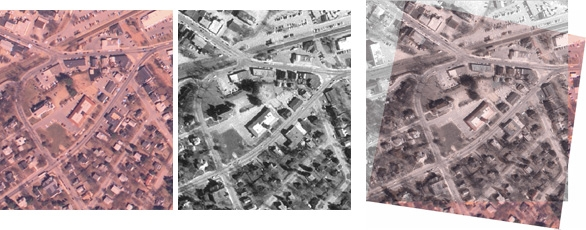
\includegraphics[width=0.80\textwidth]{images/Registering_aerial_photos}
	\caption{Registering aerial photos (\copyright\ MathWorks)}
	\label{fig:image registration example}
\end{figure}
\begin{figure}[htbp]
	\centering
	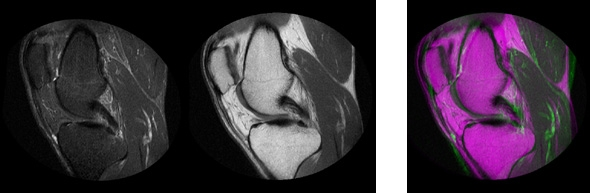
\includegraphics[width=0.80\textwidth]{images/medical_image}
	\caption{Automatic registration on multimodal medical images (\copyright\ MathWorks)}
	\label{fig:image registration example 2}
\end{figure}
In the past few decades, image acquisition devices have developed rapidly, so that the number and diversity of images obtained have increased correspondingly, which has led to the study of image registration. A comprehensive survey of image registration methods has been published in 2003 by Barbara \cite{zitovaImageRegistrationMethods2003}. Typically, the process of the most image registration technology is as follows: 
\begin{itemize}
	\item \textit{Feature detection}: Salient and distinctive objects (closed-boundary regions, edges, contours, line intersections,
corners, etc.) are manually or, preferably, automatically detected. For further processing, these features can be represented by their point representatives (centers of gravity, line endings, distinctive points).
	\item \textit{Feature matching}: The connection between corresponding features in image pair is established through this step with various feature descriptors or similarity measures along with spatial relationships.
	\item \textit{Transform model estimation}: The coordinate transformation so-called mapping function is estimated by matching features.  Image registration is performed by the mapping function.
	\item \textit{Image resampling and transformation}: In this step, one image is transformed by mapping function to another. Image values in non-integer coordinates are computed by the appropriate interpolation technique.
\end{itemize} 

\begin{figure}[htbp]
	\begin{center}
	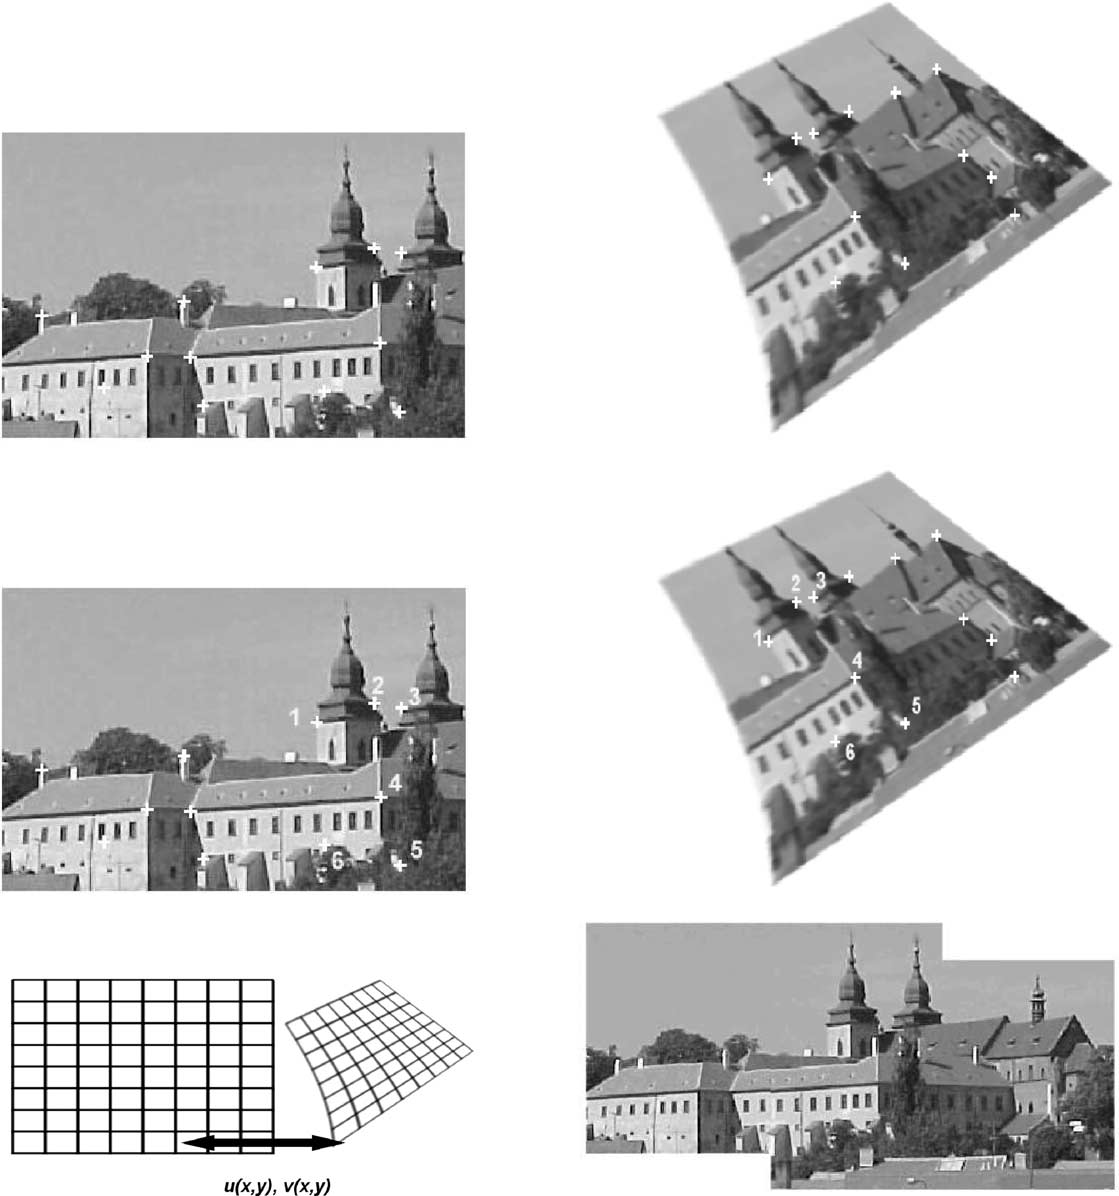
\includegraphics[width=0.80\textwidth]{images/image registration}
	\caption{Four steps of image registration}
	\label{fig:image registraion}
	\end{center}
	{\small  Top row -- feature detection (corners were used as the features in this case). Middle row -- feature matching by invariant descriptors (the corresponding pairs are marked by numbers). Bottom left -- transform model estimation exploiting the established correspondence. Bottom right -- image resampling and transformation using appropriate interpolation technique. \cite{zitovaImageRegistrationMethods2003}}
\end{figure}

Based on years of development, the current main theories of image registration can be divided into two categories: some typical dense methods seen in \cref{tab:Dense Method} and some typical sparse methods seen in \cref{tab:Sparse Method}.

\begin{table}[htbp]
	\centering
	\scriptsize  
	\begin{tabular}{p{50pt} p{300pt}}
		\toprule
		\multicolumn{2}{c}{\bfseries Dense Method}\\ \midrule
		  SGM   &  Semi-Global Matching method  performs pixel-wise matching based on Mutual Information and the approximation of a global smoothness constraint. \cite{hirschmullerAccurateEfficientStereo2005}     \\
		Correlation based Method  &  Cross-correlation is the basic statistical approach to registration. It is often used for template matching or pattern recognition in which the location and orientation of a template or pattern are found in a picture. \cite{gruenAdaptiveLeastSquares1985a}       \\ \bottomrule
	\end{tabular}
	\caption{Dense Method}  
	\label{tab:Dense Method} 
\end{table}

\begin{table}[htbp]
	\centering
	\scriptsize  
	\begin{tabular}{p{50pt} p{300pt}}
		\toprule
		\multicolumn{2}{c}{\bfseries Sparse Method}\\ \midrule
		SIFT   &  The scale-invariant feature transform (SIFT) is a feature detection algorithm in computer vision to detect and describe local features in images \cite{loweObjectRecognitionLocal1999}   \\
		ORB  &  Oriented FAST and rotated BRIEF (ORB) is a fast robust local feature detector, that  is based on the FAST key-point detector and a modified version of the visual descriptor BRIEF (Binary Robust Independent Elementary Features). \cite{rubleeORBEfficientAlternative2011}      \\ \bottomrule
	\end{tabular}
	\caption{Sparse Method}  
	\label{tab:Sparse Method} 
\end{table}

But sometimes, it's hard to tell them apart. For example, image stitching with SIFT features used the sparse feature points to estimate a dense homography. P. Hellier use simultaneously both dense and landmark-based approaches for nonrigid registration. \cite{hellierCouplingDenseLandmarkbased2003}. The Algorithm in the thesis first estimate the multiple homography matrix based on different plane patches in the image, then this series of transformation matrices could be seen as a  multiple homography matrices that is used to register the whole image..

\section{Homography} \label{sec: Multiple Homography}
The homography is a projective linear mapping, a special case of the mapping between the images of corresponding points, when those are the image points of 3D planar scene. A 2D point $\left( x, y \right)$ in an image can be represented as a 3D vector $ \rdx = \left( x_{1}, x_{2}, x_{3}\right)$ where $ x = \frac{x_{1}}{x_{3}} $ and $ y = \frac{x_{2}}{x_{3}} $. This is called the homogeneous representation of a point and it lies on the projective plane $ \dsP^{2} $ \cite{szeliskiComputerVisionAlgorithms}.  As mentioned above,  a homography is an invertible mapping of points and lines on the projective plane $ \dsP^{2} $.Other terms for this transformation include \textit{collineation}, \textit{projectivity}, and \textit{planar projective transformation}. Hartley and Zisserman \cite{hartleyMultipleViewGeometry2004} provide the specific definition that a homography is an invertible mapping from $ \dsP^{2} $ to itself such that three points lie on the same line if and only if their mapped points are also collinear. They also give an algebraic definition by proving the following \cref{thm:homography}. This tells us that in order to calculate the homography that maps each $ \rdx_{i} $ to its corresponding $ \rdx_{i}^{'} $ it is sufficient to apply a  $ 3 \times 3 $  matrix $ H $ to $\rdx_{i}$. For more mathematical derivation process, see \cref{sec:main idea}
\begin{theorem}[Homography]\label{thm:homography}
	A mapping from $\dsP^{2}\rightarrow\dsP^{2}$ is a projectivity if and only if there exists a non-singular $3\times3$ matrix $H$ such that for any point in $\dsP^{2}$ represented by vector $\rdx$ it is true that its mapped point equals $H\rdx$.
\end{theorem}

Homography have many applications in computer vision and photogrammetry: image registration, image rectification, mosaicing (\cref{fig:Homography application}) and estimation of camera motion. After extracting the camera motion from the estimated homography matrix, this information can be used for navigation, camera calibration, or to insert a 3D object model into an image or video.  The result of the proposed algorithm with the multiple homography could also be used to fundamental matrix estimation and following camera path.
\begin{figure}[htbp]
	\centering
	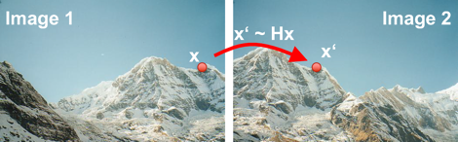
\includegraphics[width=0.80\textwidth]{images/homography_application}
	\caption{Homography application: Panorama \cite{stricker2DProjectiveTransformations2020}}
	\label{fig:Homography application}
\end{figure}

But in some situations, like remote sensing,  there are more than one flat planes in images (here mostly refers to the surface of earth) or the planes in images are not flat enough to be one plane. According to the definition of homography it can only be used for one flat plane and more than one homography matrix are needed for this case.  And this whole array of homography matrices are all intrinsically interconnected by latent variables, called multiple homography (More mathematical derivation can be found in \cref{subsec: Multiple Homography calculation}) . The algorithm is to find a set of compatible homographies between images pair.

\section{Epipolar Geometry}\label{sec:Epipolar Geometry}
The Epipolar geometry between two views is essentially the geometry of the intersection of the image planes with the pencil of planes having the baseline as axis (the baseline is the line joining the camera centres). This geometry is usually motivated by considering the search for corresponding points in stereo matching.

\cref{fig:epipolar} shows how a pixel in one image $ \rdx_{0}$ projects to an \textit{epipolar line segment} in the other image. The segment is bounded at one end by the projection of the original viewing ray at infinity $ \rdp_{\infty}$ and at the other end by the projection of the original camera center $ \rdc_{0}$ into the second camera, which is known as \textit{epipole} $\rde_{1}$. If we project the epipolar line in the second image back into the first, we get another line (segment), this time bounded by the other corresponding \textit{epipole} $\rde_{0}$. Extending both line segments to infinity, we get a pair of corresponding \textit{epipolar lines} \cref{fig:epipolar}, witch are the intersection of the two image planes with the \textit{epipolar plane} that passes through both camera centers $ \rdc_{0}$ and $ \rdc_{1}$ as well as the point of interest $ \rdp$.

Supposing now that we know only $ \rdx_{0}$, we ask how the corresponding point $ \rdx_{1}$  is constrained. The \textit{Epipolar plane} is determined by the baseline and the object $ \rdp$. From above we know that the point $ \rdx_{1}$ must lie on the line of intersection $\vec{l}_{1}$ of the \textit{epipolar plane} with the second image plane, exactly the \textit{epipolar lines} mentioned above. 
\begin{figure}[htbp]\centering
	\subfloat[]{
		\label{fig:epipolar_1}
		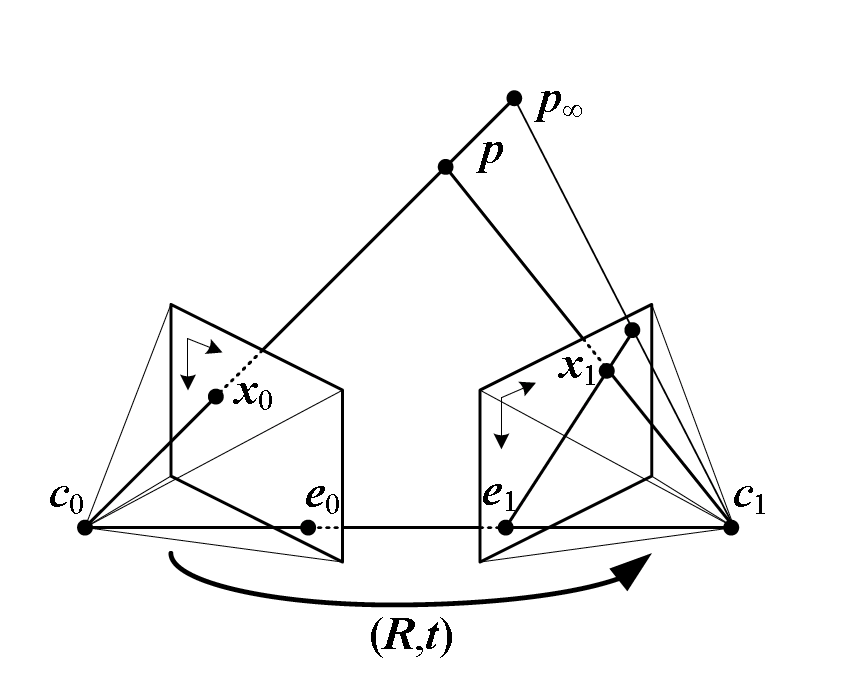
\includegraphics[width=0.40\textwidth]{./images/epipolar_1.png}
	} \qquad
	\subfloat[]{
		\label{fig:epipolar_2}
		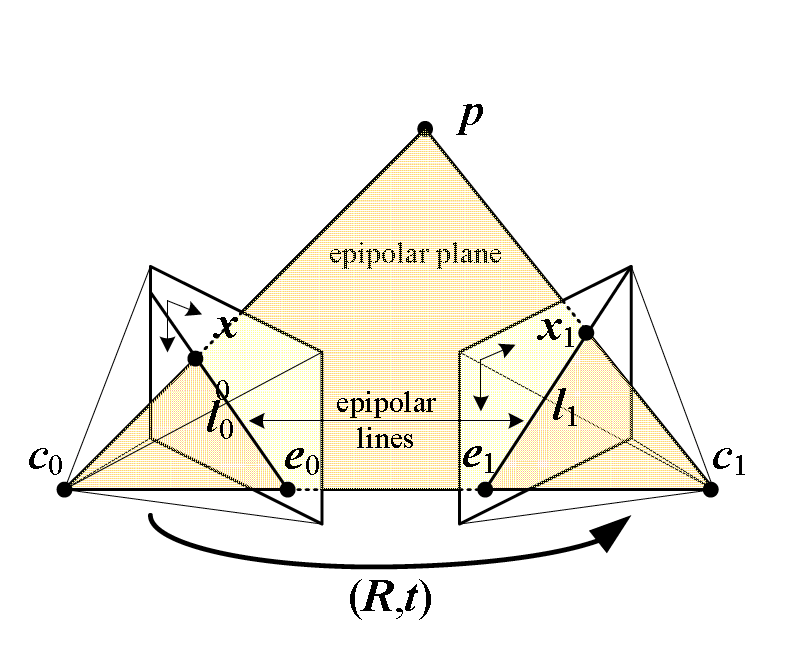
\includegraphics[width=0.40\textwidth]{./images/epipolar_2.png}
	} 
	\caption{Epipolar geometry (a) Epipolar line segment corresponding to one ray; (b) Corresponding set of epipolar lines and their epipolar plane.}
	\label{fig:epipolar}
\end{figure}

In terms of a stereo correspondence algorithm the benefit is that the search for the point corresponding to $ \rdx_{0}$ need not cover the entire image plane but can be restricted to the line $\vec{l}_{1}$. And my algorithm could also be partly proved with \textit{epipolar geometry} (seen in \cref{subsec:Rectified Stereo Images}).

\section{Least Squares Correlation}\label{sec:Least Squares Correlation}
The method of least squares is a standard approach in regression analysis to approximate the solution of over-determined systems (sets of equations which there are more equations than unknowns) by minimizing the sum of the squares of the residuals made in the results of every single equation. What's more, the least squares correlation is a very potent and flexible technique for all kinds of data matching problems. Here its detailed application process to image matching is outlined.

 Start from the most basic, linear least squares. 
\begin{definition}[Linear Least Squares]\label{thm:linear least squares}
A regression model is a linear one when the model comprises a linear combination of the parameters $\vec{\beta}=(\beta_{1}, \beta_{2}, \cdots, \beta_{n})^T$, i.e.,
\begin{align} \label{equ:model}
f(\vec{x}, \vec{\beta}) = \sum_{j=1}^{m} \beta_{j} \phi_{j}(\vec{x})
\end{align}
where the function $\phi_{j}(\vec{x}) $ is a function of input $\vec{x} = \left( x_1, x_2, \cdots, x_i\right) ^T$.

Letting $X_{ij} = \phi_{j}(x_{i})$ and putting the independent and dependent variables in matrices $X$ and $Y$ we can compute the sum of squares in the following way, note that $D$ is the set of all data: $X$ and $Y$.
\begin{align}
E(D,  \vec{\beta} ) =  \begin{Vmatrix}X\vec{\beta}- Y\end{Vmatrix}^{2}
\end{align}
Finding the minimum of it can be achieved through setting the gradient of the loss to zero and solving for $\vec{\beta}$
\begin{align}
 \frac{\partial E(D, \vec{\beta})}{\partial \vec{\beta}}  =   \frac{\partial((X\vec{\beta} - Y)^{T}(X\vec{\beta} - Y)) }{\partial \vec{\beta}}=-2X^{T}Y+2X^{T}X\vec{\beta} 
\end{align}
Finally setting the gradient of the loss to zero and solving for $\vec{\beta}$ we get:
\begin{align}
-2X^{T}Y+2X^{T}X\vec{\beta} = 0  \Rightarrow \nonumber \\
\vec{ \hat{\beta} } = (X^{T}X^{-1})^{-1}X^{T}Y
\end{align}
\end{definition}

When function $f(\vec{x}, \vec{\beta})$ represent the image mapping model, $\vec{x}$ means correspondingly the all points in the image and $\vec{\beta}$ is the parameters in the model, the process will change to an image registration process for a series of consecutive images from the video of the same scene (e.g. aerial video), since the model of image mapping according to the \cref{equ:model} is nonlinear, it is a nonlinear least square problem. This is a over-determined  problem which has more observations than the parameters.  Most algorithms involve choosing initial values for the parameters. Then, the parameters are refined iteratively i.e. the values are obtained by successive approximation. In the thesis, Gauss-Newton algorithm is used to solve this nonlinear least squares problem. 

\begin{definition}[Gauss-Newton algorithm] \label{thm:Gauss-Newton algorithm}
Given $m$ functions $\vec{r} = (r_{1}, \cdots, r_{m} )^T $(often called residuals) of n variable $\vec{\beta} = (\beta_{1}, \cdots, \beta_{n})^T $, with $m \geq n$, the Gauss-Newton algorithm iteratively finds the value of the variables that minimizes the sum of squares \cite{deuflhardLeastSquaresProblems2011}
\begin{equation}
S(\vec{\beta}) = \sum_{i=1}^m r_i^2(\vec{\beta})
\end{equation}
\end{definition}

Starting with an initial guess $\vec{\beta}^{(0)}$ for the minimum, the method proceeds by the iterations
\begin{equation}
\vec{\beta}^{(s+1)} = \vec{\beta}^{(s)} - \left(\mathbf{J_r}^{T} \mathbf{J_r} \right)^{-1} \mathbf{J_r}^{T} \vec{r}\left(\vec{\beta}^{(s)}\right)
\end{equation} 
where the entries of the Jacobian matrix it $\vec{\beta}^s$
\begin{equation}
\left(\mathbf{J_r}\right)_{ij} = \frac{\partial r_i \left(\vec{\beta}^{(s)}\right)}{\partial \beta_j}
\end{equation}

In data fitting, where the goal is to find the parameters $\vec{\beta}$ such that a given model function $y = f(\vec{x}, \vec{\beta}) $ best fits some data points$(\rdx_i,  \rdy_i)$, the function $r_i$ are the residuals:
\begin{equation}
r_i(\vec{\beta}) = y_i - f\left( \rdx_i, \vec{\beta}\right)
\end{equation}
Then, the Gauss-Newton method can be expressed in terms of the Jacobian $\mathbf{J}_f$ of the function $f$ with respect to $\vec{\beta}$ as 
\begin{equation}\label{eq:Final Gauss-Newton}
\vec{\beta}^{(s+1)} = \vec{\beta}^{(s)} + \left(\mathbf{J_f}^{T} \mathbf{J_f} \right)^{-1} \mathbf{J_f}^{T} \vec{r}\left(\vec{\beta}^{(s)}\right)
\end{equation}
Note that now the Jacobian $\mathbf{J}_f$ is for function $f$ not $r$, the sign before $\left(\mathbf{J_f}^{T} \mathbf{J_f} \right)^{-1} \mathbf{J_f}^{T} \vec{r}\left(\vec{\beta}^{(s)}\right)$ changes.






\chapter{Method}\label{ch:method}
\section{Main idea}\label{sec:main idea}
In this chapter, the algorithm, how to use homography transformation to do image registration is introduced. It will start with the camera projection to get 3D projection transformation. Then it is simplified to 2D projection with the constrains of points on a plane i.e. Homography transformation. Finally,  the algorithm of multiple homography will be introduced. 
\subsection{Projection of Points on a Plane}
Camera projection is a projection progress for a set of points from world coordinate system to image coordinate system, i.e. to calculate a projection matrix between these two coordinate system, which is called camera matrix $P$. And the exact definitions of different coordinates is in \cref{def: world coordinate system}, \cref{def: camera coordinate system}, \cref{def: image coordinate system} and \cref{def: pixel coordinate system}.

\begin{figure}[htbp]
	\centering
	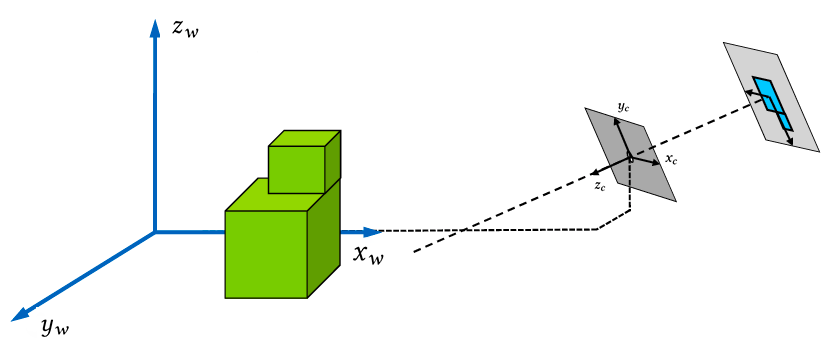
\includegraphics[width=0.80\textwidth]{images/World_to_camera}
	\caption{World to image mapping \cite{collinsPlanarHomographies}}
	\label{fig:worldtocamera}
\end{figure}

Just like \ref{fig:worldtocamera} shows, the first step is to transform from world coordinate to camera coordinate. The extrinsic parameter is the 3 by 3 rotation matrix $R$ of camera coordinate system relative to the world coordinate system and the location $\rdc$ of the camera center in the world coordinate system. The mapping is describe as: (in the equation, $\vec{0}_{3}$ means a vector of three zeros.)
\begin{align}\label{eq:world to camera}
	\begin{pmatrix}
	 		x_c\\
	 		y_c\\
	 		z_c\\
	 		1
	\end{pmatrix}=
	\begin{bmatrix}R^T & -R^T \rdc \\
		\vec{0}_{3}^T & 1
	\end{bmatrix}
	 \cdot \begin{pmatrix}
	x_w\\y_w\\z_w\\1
\end{pmatrix}
\end{align}
Then with the 3 by 3 calibration matrix $K$ (consists of intrinsic parameters), the coordinate is transformed to pixel coordinate as 
\begin{align}\label{eq:camera to pixel}
	\begin{pmatrix}
		u\\
		v\\
		1
	\end{pmatrix} \propto z_c \begin{pmatrix}
	u\\
	v\\
	1
	\end{pmatrix} = \begin{bmatrix}
	K&\vec{0}_{3}\end{bmatrix} \cdot \begin{pmatrix}
	x_c\\
	y_c\\
	z_c\\
	1
\end{pmatrix}
\end{align}
Combine \cref{eq:world to camera} and \cref{eq:camera to pixel}, 
\begin{align}
\begin{pmatrix}
u\\
v\\
1
\end{pmatrix} \propto z_c\begin{pmatrix}
u\\
v\\
1
\end{pmatrix} = \begin{bmatrix}
K&\vec{0}\end{bmatrix} \cdot \begin{bmatrix}R^T & -R^T \rdc \\
\vec{0}^T & 1 \end{bmatrix} \cdot \begin{pmatrix}
x_w\\y_w\\z_w\\1
\end{pmatrix}
\end{align}
And the middle part is the 3 by 4 camera matrix $P$, which describes the mapping of a pinhole camera from 3D points in the world to 2D points in an image.
\begin{align}
P= KR^T \begin{bmatrix}I_{3} & -\rdc \end{bmatrix}
\end{align}
Here distortion is ignored to ensure that it is a linear transformation.

When the object more specifically the points of object $\rdx$is on one plane and $\vec{n}$ is defined as the unit outward normal vector of plane, then the scalar product $\rdx \cdot \vec{n}$ is constant. Thus the camera matrix will be simplified to a 3 by 3 matrix, called homography matrix $H$. Suppose the plane is on the x-y plane in the world, detailed process of this shows in the \cref{fig:planar projection}. The homography matrix between world and image coordinate is finally simplified to:
\begin{align}
H = \begin{bmatrix}
h_{11} &h_{12} & h_{13}\\
h_{21} &h_{22} &h_{23}\\
h_{31}&h_{32}&h_{33}
\end{bmatrix}
\end{align}
\begin{figure}[htbp]
	\centering
	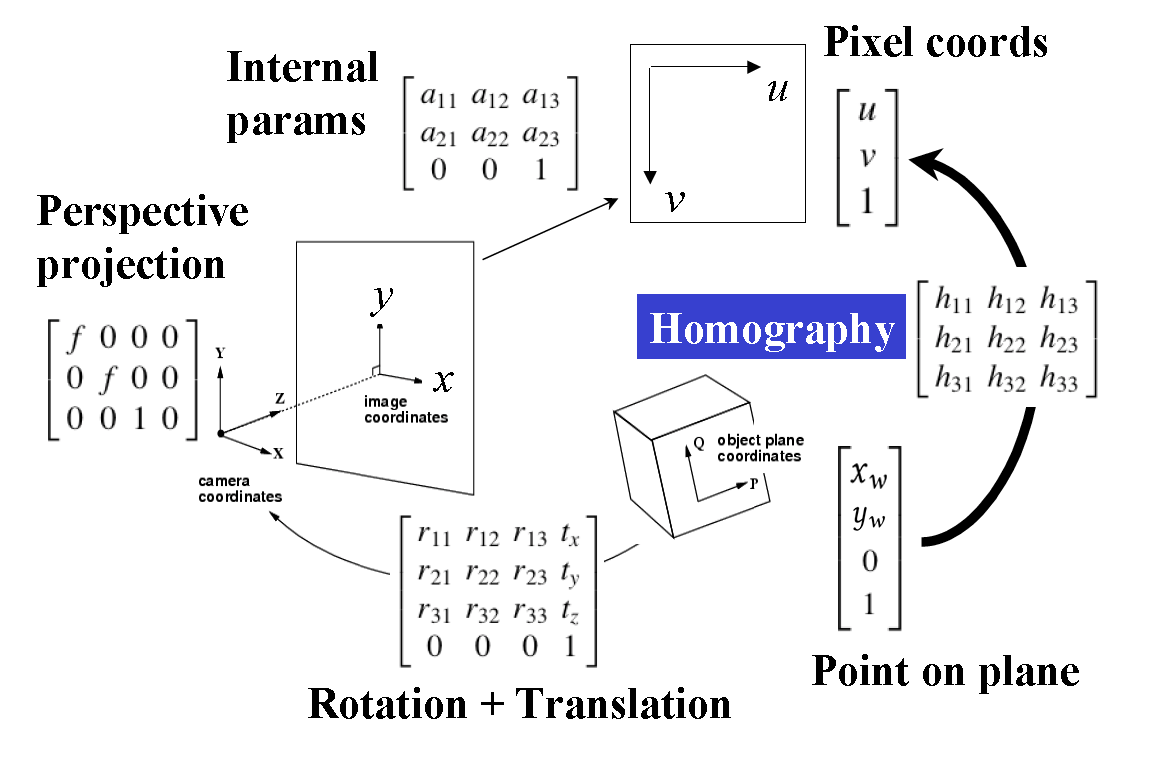
\includegraphics[width=0.80\textwidth]{./images/Planar Projection.png}
	\caption{Planar projection \cite{collinsPlanarHomographies}}
	\label{fig:planar projection}
\end{figure}
Go further, when there is a planar object in two different cameras or one camera with different poses, we can get two homography matrix $ H_{1}$ and $H_{2}$ for this two transformation. Then the homography matrix $H_{2\leftarrow1}$ between this two images of the same object can be calculate as:
\begin{align} 
H_{2\leftarrow1} = H_{2}\cdot H_{1}^{-1}
\end{align}
We assume that two fixed uncalibrated cameras give rise to two camera matrices $P_{1} = K_1R_1^T[I_3, -\rdc_{1}]$ and $P_{2} = K_{2}R_{2}^T[I_{3}, -\rdc_{2}]$. Moreover, these two cameras photograph the same plane $n$ with a unit outward normal $\vec{n}_{n}$ situated at a distance $d_{n}$ from center $\rdc_{1}$ of camera 1. Then the plane $n$ gives rise to a planar homography from the camera 1 to camera 2: \cite{chojnackiEnforcingConsistencyConstraints2015} \cite{bakerParameterizingHomographies}
\begin{align}\label{eq:homography}
H=K_{2}R_{2}^T(I-\frac{(\rdc_{2}-\rdc_{1})\vec{n}_n^{T}}{d_n})R_{1}K_{1}^{-1}
\end{align}
where  
\begin{itemize}
	\item $\rdc_{1},\rdc_{2}$ : location of the camera center in the world coordinate system
	\item $R_{1},R_{2}$: rotation matrix of camera coordinate system relative to the world
	\item $K_{1},K_{2}$: calibration matrix of camera
	\item $\vec{n}_n$: unit outward normal vector of plane
	\item $d_n$: distance from the plane to camera center $\rdc$ and $d_n = \vec{n}_n\left(\rdx - \rdc_{1}\right)$ for any point $\rdx$ on the plane
\end{itemize}

\begin{definition}[World coordinate system]\label{def: world coordinate system}
	World coordinate system $(x_w, y_w, z_w, 1)^T$is the right handed cartesian coordinate system where people take the picture . The unit is meter.
\end{definition}
\begin{definition}[Camera coordinate system]\label{def: camera coordinate system}
	Camera coordinate system $(x_c, y_c, z_c, 1)^T $ is established on the camera in order to describe the position of object from perspective of camera, as a middle link between the world coordinate system and the image/pixel coordinate system. In the thesis,  the origin is set at the center of camera in meters, $z$ axis is pointing from the center of camera to object, $y$ axis is upwards and $z$ axis points to right.
\end{definition}
\begin{definition}[Image coordinate system]\label{def: image coordinate system}
	Image coordinate system$(x, y, 1)^T$ is established on the image in order to describe how locations are measured in the image and the projection transmission relationship of the object from camera coordinate to pixel coordinate during camera projection. In the thesis, the origin is set at the center of image in meters.
\end{definition}
\begin{definition}[Pixel coordinate system]\label{def: pixel coordinate system}
	Pixel coordinate $(u, v, 1)^T$ defines the pixel location as an array in multi-dimensional space. Each image axis has a length, in pixels, so that the image coordinate run between 1 and the length of axis. The total number of pixels in the image equals the product of the axis length for all image axes. In the thesis, the origin is set at the center of the first upper left pixel in the image.
\end{definition}
And in all definitions above have used the homogeneous coordinate in projective geometry. They have the advantage that the coordinates of points, including points at infinity, can be represented using finite coordinates.
\subsection{Multiple Homography} \label{subsec: Multiple Homography calculation}
Just like in \cref{sec: Multiple Homography} introduced, when there are more than one flat planes in the image, only one homography matrix can not describe all the planes. For this situation, the multiple homography is needed. Multiplying out \cref{eq:homography} and rearranging it leads to  
\begin{align} \label{eq:Multiplehomographymatri}
	H=K_{2}R_{2}^T R_{1}K_{1}^{-1}+K_{2}R_{2}^T(\rdc_{1}-\rdc_{2})\cdot \frac{\vec{n}_n^{T}}{d_n}R_{1}K_{1}^{-1}
\end{align}
and define that,
\begin{itemize}
	\item $H_{\infty}=K_{2}R_{2}^T R_{1}K_{1}^{-1}$
	\item $\vec{e}=K_{2}R_{2}^T(\rdc_{1}-\rdc_{2})$
	\item $\vec{q}_{n}^T=\frac{\vec{n}_n^{T}}{d_n}R_{1}K_{1}^{-1}$
\end{itemize}
Among them, $H_{\infty}$ represent the homography matrix for the plane at infinity, $\vec{e}$ is the epipole in the second view, and $\vec{q}_n$ means a $3 \times 1$ vector for the plane $n$, which all the points belongs to. Finally, the homography matrix for plane $n$ is
\begin{align}\label{eq:homography_infty}
	H_{n} = H_{\infty} + \vec{e} \cdot \vec{q}_{n}^T
\end{align}

If the homography $H_{\infty}$ at infinity can't be found,  a homography matrix $H_{0}$ for an exist plane can be used as reference plane and all other planes can be expressed in terms of $H_0$ with:
\begin{align}\label{eq:homography_0}
H_{0} = H_{\infty} + \vec{e} \cdot \vec{q}_{0}^T
\end{align}
And for another plane $n$ in the same image, $\vec{p}_{n}^T$ is defined as $\vec{p}_{n}^T = \vec{q}_{n}^T -\vec{q}_{0}^T$. With \cref{eq:homography_0}, the new form of homography matrix for plane $n$ is got
\begin{align}\label{eq:homography_i}
	H_{n} = H_{0} + \vec{e} \cdot \vec{p}_{n}^T
\end{align}
In this equation, $H_{0}$ is a global and constant value for the whole image, $\vec{e}$ is also a global variable (the epipole in the second view) for the whole image. And $\vec{p}_{n}^T$ is different for different planes. Therefore,  \cref{eq:homography_i} is an express of multiple homography with two global variables $H_{0}$, $\vec{e}$ and one local variable $\vec{p}_{n}^T$. People can use it to transform the plane in one image to another or build the corresponding matching for the same plane in different images.  The algorithm also use this multiple homography to transform the plane and make image registration per plane.


\section{Derivation of the algorithm}\label{sec:Implementation}
The derivation of the algorithm of the thesis is shown in this section. First, I apply the theories and methods mentioned before on the image registration process to get my algorithm. After that, the application of my algorithm to a simple case with rectified stereo images is shown. In the end, my algorithm is applied to the unrectified images i.e. arbitrary images.
\subsection{Image registration Process}
Similar images are created in many situations, such as from stereo cameras, map updating and motion detection. Image registration process can be applied on this similar images to match or register the same structure or patches in both images. And the algorithm is a kind of image registration algorithm to register the plane patches in images with the multiple homography approach.

In order to introduce the algorithm, we assume that there is a pair of images with same plane patches, which are from the stereo cameras or consecutive images from the aerial video. Let the two images be $I_1$ and $I_2$ where we call $I_1$ the "template image" and $I_2$ the "target image". The template image is is formulated as the brightness function $I_1(\rdx'_{ij})$, in which $\rdx'_{ij}$ means the pixel coordinate of the pixel at row $i$ and column $j$. And the target image is defined as $I_2(\rdy'_{ij})$, in which $\rdy'_{ij}$ means the pixel coordinate of the point in target image, which is corresponding to the point $\rdx'_{ij}$ in template image. The symbol $I_1$ and $I_2$ here represent respectively the function that can transform the coordinate variable to pixel value, i.e. $I$ transform the variable in space $\dsR^{2}$ to space $\dsR$(In the thesis, only gray-scaled images is consider for simplicity. But the generalization to color images is not complicated, applying the algorithm on three channels of the image separately and add them up finally). Further more, we will use the homography transformation per patch to do the registration separately, so function $T_n$ represents the process of homography transformation from space $\dsR^{3}$ to space $\dsR^3$ with homogeneous coordinate for plane patch $n$. Here we define $T_n$ for plane patch $n$ from template to target image.

But a problem comes now, the output of $T_n$ is a 3-length vector in $\dsR^3$ space, the input of $I_2$ is paradoxically a 2-length vector in $\dsR^2$ space. So we still need a dehomogenization function to connect them to describe the transformation process. Therefore, we introduce the function $N$ to do dehomogenization transformation:
\begin{align} \label{eq:N}
	\rdx'_{ij} = N(\rdx_{ij}) \\
	\rdy'_{ij} = N(\rdy_{ij})
\end{align}
where $\rdx_{ij}$($\rdy_{ij}$) and ${\rdx_{ij}}'$(${\rdy_{ij}}'$)  are homogeneous coordinate and Cartesian coordinate of pixel in template image(target image).

From the \cref{eq:homography_infty}, the corresponding pixels in the plane region $n$ of template and target image can be connected as:
\begin{align}
	\rdy_{ij} & = H_n \cdot \rdx_{ij} \nonumber \\
			& = (H_{\infty} + \rde \cdot \vec{q}_{n}^T) \rdx_{ij}
\end{align}	
where $\rdx_{ij} = (\rdx'_{ij}, 1)^T$ and $\rdx_{ij}$ means the $i$ row $j$ column in every patch. $H_\infty$ and $\vec{q}_{n}^T$ are used in the calculation process. If they can't be found in real application, they could be replaced by arbitrary existing $H_0$ and $\vec{p}^T_n$ as \cref{eq:homography_i} shown. Then function $T_n$ can be expressed as 
\begin{align}
	T_n(H_{\infty}, \rde, \vec{q}_n, \rdx_{ij}) & = (H_{\infty} + \rde \cdot \vec{q}_{n}^T) \rdx_{ij}
\end{align}
So in this way, a projection of planar region from target to template image has been established. 
\begin{align}\label{eq:I_2}
I_2(N(T_n(H_{\infty}, \rde, \vec{q}_n, \rdx_{ij})))
\end{align}

After getting the mapping model, we have to get an estimation of the variable in it to ensure the accuracy of mapping. According to the \cref{sec:Least Squares Correlation}, the method Least Squares Correlation is used to solve this problem. Because the function $I$ is nonlinear, Gauss-Newton algorithm is utilized. 

As stated in \cref{thm:Gauss-Newton algorithm}, most algorithms involve choosing initial values for the parameters. Then, the parameters are refined iteratively. In our application scenario, the parameter is defined as 
\begin{align}\label{eq:beta}
	\vec{\beta} =  \begin{pmatrix}\operatorname {vec}(H_\infty)\\\rde\\ \vec{q}_n \end{pmatrix}
\end{align}
 And the dimension of $\vec{\beta}$ is $s$. Then the values are obtained by successive approximation:
\begin{align}
	\vec{\beta}^{(k+1)} =  \vec{\beta}^{(k)} + \Delta \vec{\beta}
\end{align}
where a superscript $k$ is an iteration number, and the vector of increments $\Delta \vec{\beta}$ is called the shift vector.  For the convenience of expression, we name function $I_2(N(T_n(\vec{\beta}, \rdx_{ij})))$ as $F_n(\vec{\beta}, \rdx_{ij})$. At each iteration the transformation model $F_n(\vec{\beta}, \rdx_{ij})$ is linearized by approximation to a first-order Taylor series expansion around $\vec{\beta}^{(k)}$:
\begin{align}
	F_n(\vec{\beta}^{(k+1)}, \rdx_{ij}) &\approx F_n^(k)(\vec{\beta}^{(k)}, \rdx_{ij})+ \sum_{u=1}^s \frac{\partial F_n(\vec{\beta}, \rdx_{ij})}{\partial \beta_u} \left({\beta_u}^{(k+1)}-{\beta_u}^{(k)} \right) \nonumber \\
	& \approx F_n^(k)(\vec{\beta}^{(k)}, \rdx_{ij}) + \sum_{u=1}^s j_{nu}\Delta\beta_u
\end{align}
where 
\begin{align} \label{eq:Jacobian}
j_{nu} = \frac{\partial F_n(\vec{\beta}, \rdx_{ij})}{\partial \beta_u}
\end{align}
as the coefficient of the Jacobian.

We define mapping error $e_{nij}$ of pixel $\rdx_{ij}$ of template image in patch $n$ as
\begin{align}\label{eq:e}
	e_{nij}^{(k+1)} & = I_1(N(\rdx_{ij}))- F^{(k+1)}_n(\vec{\beta}^{(k+1)}, \rdx_{ij}) \nonumber \\
	   & = I_1(N(\rdx_{ij})) - F_n^{(k)}(\vec{\beta}^{(k)}, \rdx_{ij}) - \sum_{u=1}^s j_{nu}\Delta\beta_u \nonumber \\
	   & = I_1(N(\rdx_{ij})) - F_n^{(k)}(\vec{\beta}^{(k)}, \rdx_{ij}) - \mathbf{J}_{F_n} \Delta\vec{\beta_s}
\end{align}
where the Jacobian $\mathbf{J}_{F_n}$ denotes a vector with entries $j_{nu}$ for $u$ running from $1$ to $s$. It changes for each iteration. $\Delta\vec{\beta_s}$ consists of the changes of all elements in $\vec{\beta}$

Our aim is to minimize the mapping error. When the gradient for $\vec{\beta}$ of \cref{eq:e} is set to zero, $e$ gets the minimum value. When we applied the above equation on all pixels in all plane patches. Then $t$ is the total number of the pixels in all patches and the parameter for $\vec{q}_n$ will change to a big vector  $\vec{Q} = (\vec{q}_1^T, \vec{q}_2^T, \cdots, \vec{q}_n^T)^T$, which contains all $\vec{q}_n$ for all patch $n$. Obviously, the dimension of $\vec{Q}$ is $3n$.  $\vec{E}$ is defined as the combination of all $\vec{e}_{nij}$ in vector. The combination of $F_n$ is $F(\vec{\beta}, \rdx_{ij}) = (F_1, F_2, \cdots, F_n)^T$. 
According to \cref{eq:Final Gauss-Newton}, the result comes to:
\begin{align}
	\vec{\beta}^{(k+1)} = \vec{\beta}^{(k)} + \left(\mathbf{J}_{F}^{T} \mathbf{J}_{F} \right)^{-1} \mathbf{J}_{F}^{T} \vec{E}^{(k)}
\end{align}

Now, the only left thing is the initialization of the parameters. The algorithm is applied on stereo images or the consecutive images from the video. So there must be EXIF information in the metadata. We have an estimation of the camera positions $\rdc_1, \rdc_2$ from the GPS, and an estimation of the camera rotation $R_1, R_2$ from the INS, and an estimation of $K_1, K_2$ from the image size and field-of-view reported by the camera. With this we can get already an estimate of $H_\infty$ and $\rde$ by \cref{eq:Multiplehomographymatri}. Moreover, we know approximately where the plane is in the image, this gives us also an estimate of $\vec{q}_n$. (This is the job of preprocessing. What I got is the position of planes, so the plane patches are chosen currently by hand.) And the flow chart of this process is shown in \cref{fig:work_flow_gauss_newton}. 
\begin{figure}[tbp]
	\centering
	\tikzsetnextfilename{work_flow_gauss_newton.tex}
	\tikzset{external/export next=false}

\tikzstyle{startstop} = [rectangle, rounded corners, minimum width=3cm, minimum height=1cm,text centered, draw=black, fill=red!30]
\tikzstyle{io} = [trapezium, trapezium left angle=70, trapezium right angle=110, minimum width=3cm, minimum height=1cm, text centered, text width=4cm, draw=black, fill=blue!30]
\tikzstyle{process} = [rectangle, minimum width=3cm, minimum height=1cm, text centered, text width=4cm, draw=black, fill=orange!30]
\tikzstyle{decision} = [diamond, minimum width=3cm, minimum height=1cm, text centered, text width=4cm, draw=black, fill=green!30]
\tikzstyle{arrow} = [thick,->,>=stealth]



\begin{tikzpicture}[node distance = 2cm, auto]
% Place nodes
\node [startstop] (start) {Start};
\node (init) [io, below of=start] {Initialization: $k = 0, \vec{\beta}^{(0)}$};
\node (e) [process, below of=init] {Mapping error: $\vec{E}^{(k)}  = I_1(N(x_{ij}))- F^{(k)}(\vec{\beta}^{(k)}, \rdx_{ij})$};
\node (dec) [decision, below of=e, yshift=-2cm] {$\left | E^{(k-1)}-E^{(k)} \right | \leq Threshold$};
\node (final-beta) [process, below of=dec, yshift=-2cm] {Final Result: $\vec{\beta}_{final} = \vec{\beta}^{(k)} $};
\node (stop) [startstop, below of=final-beta] {Stop};
\node (Joca) [process, right of=dec, xshift=6cm] {Jacobian Calculating: $\mathbf{J}_{F}$};
\node (beta-up) [process, above of=Joca] {$\vec{\beta}$ updating: $\vec{\beta}^{(k+1)} = \vec{\beta}^{(k)} + \left(\mathbf{J}_{F}^{T} \mathbf{J}_{F} \right)^{-1} \mathbf{J}_{F}^{T} \vec{E}^{(k)}$};
\node (k-up) [process, above of=beta-up] {$k$ updating: $k=k+1$};


% Draw edges
\draw [arrow] (start) -- (init);
\draw [arrow] (init) -- (e);
\draw [arrow] (e) -- (dec);
\draw [arrow] (dec) -- node[anchor=east]{True}(final-beta);
\draw [arrow] (final-beta) -- (stop);
\draw [arrow] (dec) -- node[anchor=south]{False}(Joca);
\draw [arrow] (Joca) -- (beta-up);
\draw [arrow] (beta-up) -- (k-up);
\draw [arrow] (k-up) -- (e);
%\path [line] (init) -- (identify);
%\path [line] (identify) -- (evaluate);
%\path [line] (evaluate) -- (decide);
%\path [line] (decide) -| node [near start] {yes} (update);
%\path [line] (update) |- (identify);
%\path [line] (decide) -- node {no}(stop);
%\path [line,dashed] (expert) -- (init);
%\path [line,dashed] (system) -- (init);
%\path [line,dashed] (system) |- (evaluate);
\end{tikzpicture}
	
	\caption{Flow chart of Gauss-Newton algorithms}
	\label{fig:work_flow_gauss_newton}
\end{figure}



\subsection{Iterative process}
	
In the iterative process, there is a  left peseudoinverse of $\mathbf{J_{F}}^{T}$. It's difficult to solve for all the parameters in $\vec{\beta}$, but when  the parameter $\vec{\beta}$ is taken apart to optimize, the computational complexity of the total peseudoinverse will be significantly reduced (without proof). On the basis of \cref{subsec: Multiple Homography calculation}, the parameters in $\vec{\beta}$ can be divided into tow parts, global variables $H_\infty$ and $\rde$ and local variables $\vec{q}_n$. 

In this way, $\vec{Q}$ is optimized per patches separately with constant $H_\infty$ and $\rde$ after the initialization. Then $H_\infty$ and $\rde$ for all patches can be refined, when we assume $\vec{Q}$ for all patches obtained by the previous step to be fixed . The optimized iterative process is shown in \cref{fig:optimized iterative process}. And the step "Optimize $\vec{Q}^k$" and "Optimize $H_\infty^{k}, \rde^k$" can be done like the way in \cref{fig:work_flow_gauss_newton}.

Next we need to deal with the calculation about function $F_n$ in details. The Jacobian matrix $J_F$ is needed in every iterative step. Put $j_{nu}$ (\cref{eq:Jacobian}), $I_2$ (\cref{eq:I_2}), $\vec{\beta}$ (\cref{eq:beta}) and the definition of $F_n$ together and use the chain rule to calculate the derivative:
\begin{align}\label{eq:jnuR}
	j_{nu} &= \frac{\partial F_n(\vec{\beta}, \rdx_{ij})}{\partial \beta_u} \nonumber \\
				&= \frac{\partial I_2(N(T_n(\vec{\beta}, \rdx_{ij})))}{\partial \beta_u} \nonumber \\
				&= \frac{\mathrm{d} I_2(N)}{\mathrm{d}N} \frac{\mathrm{d} N(T_n)}{\mathrm{d} T_n} \frac{\partial T_n(\vec{\beta}, \rdx_{ij})}{\partial \beta_u} 
\end{align}

In order to get $j_{nu}$, we have to first to calculate $ \frac{\mathrm{d} I_2(N)}{\mathrm{d}N}$ and  $\frac{\mathrm{d} N(T_n)}{\mathrm{d} T_n}$, then $\frac{\partial T_n(\vec{\beta}, \rdx_{ij})}{\partial \beta_u}$. Here $d$ and $\partial $ both denote the Jacobian, but $d$ means there is derivative of only one vector parameter and $\partial$ means derivative of one of vector parameters. From the definition of function $N$ (\cref{eq:N}), the output of it is a 2-length vector $\rdy_{ij} = (y_i, y_j)^T$, which represents the position of the corresponding pixel in image $I_2$. So the first term $\frac{\mathrm{d} I_2(\rdy_{ij})}{\mathrm{d}\rdy_{ij}}$ means the gradient of image intensity function. It can be approximated by some differentiation operator. We will come back to this in the \cref{sec:Image derivatives}.

We start to solve the second term $\frac{\mathrm{d} N(T_n)}{\mathrm{d} T_n}$. The result of function $T_n(\vec{\beta})$ is a homogeneous coordinate $\vec{t} = (t_1, t_2, t_3)^T$ of corresponding pixel in image $I_2$ and $N(\vec{t}) = \vec{t_{12}}/t_3$. 
\begin{align} \label{eq:n}
	\frac{\mathrm{d} N(T_n)}{\mathrm{d} T_n} &= \frac{\mathrm{d}N(\vec{t})}{\mathrm{d} \vec{t}} = \frac{\mathrm{d}(t_3^{-1}\cdot \vec{t}_{12})}{\mathrm{d}\vec{t}} \nonumber \\
	&= {t_3}^{-1} \cdot \frac{\mathrm{d} \vec{t}_{12}}{\mathrm{d} \vec{t}} +  \vec{t}_{12} \cdot \frac{\mathrm{d} t_3^{-1}}{\mathrm{d}\vec{t}} \nonumber \\
	& = {t_3}^{-1} \cdot \frac{\mathrm{d} \vec{t}_{12}}{\mathrm{d} \vec{t}} - t_3^{-2}\cdot \vec{t}_{12} \cdot \frac{\mathrm{d} t_3}{\mathrm{d} \vec{t}}\nonumber \\
	&= t_3^{-1}\frac{\mathrm{d}\left(\begin{bmatrix}1 & 0 &0 \\ 0 & 1 & 0 \end{bmatrix} \cdot \vec{t}\right)}{\mathrm{d} \vec{t}} - t_3^{-2}\cdot \vec{t}_{12} \cdot \frac{\mathrm{d} \left(\begin{bmatrix} 0 & 0 & 1 \end{bmatrix}\cdot \vec{t}\right)}{\mathrm{d} \vec{t}}\nonumber \\
	&= t_3^{-1}\begin{bmatrix}1 & 0 &0 \\ 0 & 1 & 0 \end{bmatrix} - t_3^{-2}\cdot \vec{t}_{12} \cdot \begin{bmatrix} 0 & 0 & 1 \end{bmatrix}\nonumber \\
	&=  t_3^{-1} \cdot \begin{bmatrix} I_2 & - \vec{t}_{12}/t_3 \end{bmatrix} \nonumber \\
	& = t_3^{-1} \cdot \begin{bmatrix} I_2 & - N(\vec{t}) \end{bmatrix}
\end{align}
where $\vec{t}_{12} $ means $ (t_1, t_2)^T$

\begin{figure}[tbp]
	\centering
	\tikzsetnextfilename{flow_chart_optimized_iterative_process.tex}
	\tikzset{external/export next=false}

\tikzstyle{startstop} = [rectangle, rounded corners, minimum width=3cm, minimum height=1cm,text centered, draw=black, fill=red!30]
\tikzstyle{io} = [trapezium, trapezium left angle=70, trapezium right angle=110, minimum width=3cm, minimum height=1cm, text centered, text width=4cm, draw=black, fill=blue!30]
\tikzstyle{process} = [rectangle, minimum width=3cm, minimum height=1cm, text centered, text width=4cm, draw=black, fill=orange!30]
\tikzstyle{decision} = [diamond, minimum width=3cm, minimum height=1cm, text centered, text width=4cm, draw=black, fill=green!30]
\tikzstyle{arrow} = [thick,->,>=stealth]



\begin{tikzpicture}[node distance = 2cm, auto]
% Place nodes
\node [startstop] (start) {Start};
\node (init) [io, below of=start] {Initialization: $k=0, H_\infty^{0}, \vec{e}^0,  \vec{Q}^0$};
\node (E) [process, below of=init] {Mapping error: $\vec{E}^{(k)}  = I_1(N(x_{ij}))- F^{(k)}(H_\infty^{k}, \vec{e}^k,  \vec{Q}^k, \rdx_{ij})$};
\node (dec) [decision, below of=E, yshift=-3cm] {$\left | E^{(k-1)}-E^{(k)} \right | \leq Threshold$};
\node (final-beta) [process, below of=dec, yshift=-3cm] {Final Result: $H_\infty=H_\infty^{k}, \vec{e}=\vec{e}^k,  \vec{Q}=\vec{Q}^k$};
\node (stop) [startstop, below of=final-beta] {Stop};
\node (Q-optimize) [process, right of=dec, xshift=5cm]{Optimize $\vec{Q}^{k+1}$ per patch seperately with constant $H_\infty^{k}, \rde^k$};
\node (He-optimize) [process, above of=Q-optimize, yshift=0.5cm] {Optimize $H_\infty^{k+1}, \rde^{k+1}$ for all patches with constant $\vec{Q}^{k+1}$};
\node (k) [process, above of=He-optimize, yshift=0.5cm] {Next Cycle: $k = k+1$};

% Draw edges
\draw [arrow] (start) -- (init);
\draw [arrow] (init) -- (E);
\draw [arrow] (E) -- (dec);
\draw [arrow] (dec) -- node[anchor=east]{True}(final-beta);
\draw [arrow] (final-beta) --(stop);
\draw [arrow] (dec) -- node[near start]{False}(Q-optimize);
\draw [arrow] (Q-optimize) -- (He-optimize);
\draw [arrow] (He-optimize) -- (k);
\draw [arrow] (k) -- (E);
\end{tikzpicture}
	
	\caption{Flow chart of optimized iterative process}
	\label{fig:optimized iterative process}
\end{figure}

Finally, the third part $\frac{\partial T_n(\vec{\beta}, \rdx_{ij})}{\partial \beta_u}$. Because $\vec{\beta}$ contains three parts: $\operatorname {vec}(H_\infty)$, $\rde$ and $\vec{q}_n$ (\cref{eq:beta}),  $\frac{\partial T_n(\vec{\beta_u})}{\partial \beta}$ is calculated also in three situations. 
\begin{enumerate}
	\item $\beta =  \operatorname {vec}(H_\infty)$ 
	\item $\beta = \rde$ 
	\item $\beta = \vec{q}_n$ 
\end{enumerate}

When $\beta_u =  \operatorname {vec}(H_\infty)$, 
\begin{align}\label{eq:H_infty}
\frac{\partial T_n(\vec{\beta})}{\partial \operatorname {vec}(H_\infty)} & = \frac{\partial ((H_{\infty} + \rde \vec{q}_{n}^T) \cdot \rdx_{ij})} {\partial \operatorname {vec}(H_\infty)} \nonumber \\
	& = \frac{\partial ((H_{\infty} \cdot x_{ij} + e \vec{q}_{n}^T \rdx_{ij}) )}{\partial \operatorname {vec}(H_\infty)}  \nonumber \\
	& = \frac{\partial (H_{\infty} \rdx_{ij})} {\partial \operatorname {vec}(H_\infty)}
\end{align}
since $e \vec{q}_{n}^T \rdx_{ij}$ is independent from $\operatorname {vec}(H_\infty)$. 

Here it comes to matrix differentiation. And I have used the kronecker product to solve this differentiation. The definition of Kronecker product is first introduced.
\begin{definition}[Kronecker product]\label{def:Kronecker product}
	Let $A \in \dsR^{m \times n}$, $B \in \dsR^{p \times q}$. Then the \textbf{kronecker product} (or tensor product ) of $A$ and $B$ is defined as the matrix
	\begin{align}
		A \otimes B = \begin{bmatrix}
			a_{11} {B} & \cdots & a_{1n}{B} \\
			\vdots & \ddots &           \vdots \\
			a_{m1} {B} & \cdots & a_{mn} {B}
		\end{bmatrix} \in \dsR^{mp \times nq}
	\end{align}
\end{definition}
\begin{theorem}[Vectorization of matrix product]\label{def:Matrix equation}
	For any three matrices $A$, $B$, and $C$ for which the matrix product $ABC$ is defined,
	\begin{align} \label{eq:kronecker product}
		\operatorname {vec}(ABC) = (C^T \otimes A)\operatorname {vec}(B)
	\end{align}
\end{theorem}

Write \cref{eq:H_infty} as
\begin{align}\label{eq:vecH}
	\frac{\partial T_n(\vec{\beta})}{\partial \operatorname {vec}(H_\infty)} &= \frac{\partial (H_{\infty} \rdx_{ij})} {\partial H_\infty} \nonumber \\
	& =  \frac{\partial \operatorname {vec}(H_{\infty} \rdx_{ij})} {\partial \operatorname {vec}(H_\infty)} \nonumber \\
	& = \frac{\partial \operatorname {vec}(I_3 H_{\infty} \rdx_{ij})} {\partial \operatorname {vec}(H_\infty)}
\end{align}
Since \cref{def:Matrix equation}, \cref{eq:vecH} can be rewritten in the form
\begin{align}\label{eq:H_infty2}
	\frac{\partial T_n(\vec{\beta})}{\partial \operatorname {vec}(H_\infty)} & =  \frac{\partial ((\rdx_{ij}^T \otimes I_3)\operatorname {vec}( H_{\infty}))} {\partial \operatorname {vec}(H_\infty)} \nonumber \\
	& = \rdx_{ij}^T \otimes I_3
\end{align}

When $\beta =  \rde$, 
\begin{align}\label{eq:e1}
	\frac{\partial T_n(\vec{\beta})}{\partial \rde} & = \frac{\partial ((H_{\infty} + \rde \vec{q}_{n}^T) \cdot \rdx_{ij})} {\partial \rde} \nonumber \\
	& = \frac{\partial (H_{\infty} \rdx_{ij} + \rde \vec{q}_{n}^T \rdx_{ij} )}{\partial \rde}  \nonumber \\
	& = \frac{\partial (\rde \vec{q}_{n}^T \rdx_{ij})} {\partial \rde} \nonumber \\
	& = I_3 \vec{q}_{n}^T \rdx_{ij}
\end{align}
since $H_\infty$ and $\rdx_{ij}$ is independent of $\rde$


When $\beta = \vec{q}_n$,
\begin{align}\label{eq:q_n}
	\frac{\partial T_n(\vec{\beta})}{\partial \vec{q}_n} & = \frac{\partial ((H_{\infty} + \rde \vec{q}_n^T) \cdot \rdx_{ij})} {\partial \vec{q}_n} \nonumber \\
	& = \frac{\partial (H_{\infty} \rdx_{ij} + \rde \vec{q}_n^T \rdx_{ij})}{\partial \vec{q}_n}  \nonumber \\
	& = \frac{\partial (\rde \vec{q}_n^T \rdx_{ij})} {\partial \vec{q}_n} \nonumber \\
	& = \frac{\partial (\rde \rdx_{ij}^T \vec{q}_n)} {\partial \vec{q}_n} \nonumber \\
	& = \rde \rdx_{ij}^T
\end{align}

So far, we have completed the entire calculation process and can iteratively solve it.
\subsection{Radiometric Correction}\label{subsec:Radiometric Correction}
The algorithm is based on least squares correlation. But it cannot properly respond to many facts that are inseparable from the stereo images of three-dimensional and sometimes even two-dimensional objects. The conjugate images created under the perspective projection rule may be very different from each other.

The terrain gradient, height difference and position and attitude differences of the sensors may cause geometric distortions. Illumination and reflection conditions may distort the image radiometrically. Under certain conditions, this may even trigger geometric displacement. The noise and sampling rate of electronic components may also affect the geometrical and radiometric correspondence of the images. 

For aerial images, the energy that sensors on aircraft or satellites record can differ from the actual energy emitted or reflected from a surface on the ground. This is due to the sun's azimuth and elevation and atmospheric conditions that can influence the energy observed by the sensor. There, in order to obtain the real or true ground radiance or reflectance values, radiometric errors must be accounted for. And the algorithm works fast and well if the patches to be matched contain enough signal without too much high-frequency content and if geometrical and radiometric distortions are kept at a minimum. Both conditions are often not encountered in standard aerial images. Therefore radiometric correction is required for the algorithm.

Radiometric correction is a technique to reconstruct physically calibrated values by correcting the spectral distortions caused by sensors , sun angle, topography and the atmosphere as shown in \cref{fig:Radiometric Correction}.
\begin{figure}[tbp]
	\centering
	\tikzsetnextfilename{Radiometric_Correction.tex}
	\tikzset{external/export next=false}

\tikzset{
	basic/.style  = {draw, text width=2cm, drop shadow, font=\sffamily, rectangle},
	root/.style   = {basic, rounded corners=2pt, thin, align=center,
		fill=green!30},
	level 2/.style = {basic, rounded corners=6pt, thin, align=center, fill=green!60,
		text width=6.5em},
	level 3/.style = {basic, thin, align=left, fill=pink!60, text width=9em}
}

\begin{tikzpicture}[
level 1/.style={sibling distance=50mm},
edge from parent/.style={->,draw},
>=latex]

% root of the the initial tree, level 1
\node[root] {Radiometric Correction}
% The first level, as children of the initial tree
child {node[level 2] (c1) {Sensor Calibration}}
child {node[level 2] (c2) {Sun Angle /Surface Slope}}
child {node[level 2] (c3) {Atmospheric Correction}};

% The second level, relatively positioned nodes
\begin{scope}[every node/.style={level 3}]
\node [below of = c1, xshift=30pt] (c11) {Sensitivity of Detectors};
\node [below of = c11] (c12) {Vignetting Effecting};

\node [below of = c2, xshift=25pt] (c21) {Sun Angle Effect};
\node [below of = c21] (c22) {Topographic Effect};

\node [below of = c3, xshift=25pt] (c31) {Topographic Effect};
\node [below of = c31] (c32) {Scattering};
\end{scope}

% lines from each level 1 node to every one of its "children"
\foreach \value in {1,2}
\draw[->] (c1.195) |- (c1\value.west);

\foreach \value in {1,2}
\draw[->] (c2.195) |- (c2\value.west);

\foreach \value in {1,2}
\draw[->] (c3.195) |- (c3\value.west);
\end{tikzpicture}

	
	\caption{Radiometric correction}
	\label{fig:Radiometric Correction}
\end{figure}

Radiometric correction is classified into two types: absolute and relative correction.:

\textbf{Absolute correction:} Correct radiance or reflectance should be measured or converted by using the sensor calibration data, the sun angle and view angle, atmospheric models and ground truth data. The incident energy input to sensors should be analyzed correctively by radiometric correction. However it can not be applied in most applications, therefore the relative correction is applied because the atmospheric model is so complicated and the exact measurement of atmospheric condition is difficult. 

\textbf{Relative correction:} Relative correction is to normalize multi-temporal data taken on different dates to a selected reference data at specific time. The following techniques \cref{tab:Relative Radiometric Correction} will be typical.

My thesis is not mainly about radiometric correction, I only want to reduce the influence of radiometric distortion on my algorithm. So I just choose the least square method to eliminate its influence and make my algorithm more accurate. The specific application process is shown below.

In my case, $I_1$ or $I_2$ should be normalized. I choose $I_1$ here for convenience. Because if $I_2$ is chosen, then a linear function $R = r_1 I_2(N(T_n)) + r_2 $ will replace $I_2(N(T_n))$. It will cause some more calculation. 

\begin{table}[htbp]
	\centering
	\scriptsize  
	\begin{tabular}{p{80pt} p{260pt}}
		\toprule
		\multicolumn{2}{c}{\bfseries Relative Radiometric Correction}\\ \midrule
		Adjustment   &  Adjustment of average and standard deviation values.\\
		\addlinespace[3pt]
		Conversion to normalized index  &  The normalized difference vegetation index. \\
		\addlinespace[3pt]
		Histogram matching &  The histograms per band and/or per sensor are calculated and the cumulative histogram with cut-offs at $1\%$ and $99\%$ will be relatively adjusted to the reference histogram. \\
		\addlinespace[3pt]
		Least square method & linear function of $y = ax + b$ is determined, where $y$ is reference data and $x$ is data to be normalized. \\ \bottomrule
	\end{tabular}
	\caption{Relative Radiometric Correction}  
	\label{tab:Relative Radiometric Correction} 
\end{table}

After the linear function of $I_1(\rdx_{ij})$ for different plane patches $n$ is defined as $R_n(I_1) = {r_1}_n I_1 + {r_2}_n$, the mapping error $e_{nij}$ (\cref{eq:e} is changed to 
\begin{align}
	e_{nij}^{(k+1)} &= R_n^{K+1}(I_1(\rdx_{ij}))- I_2(N(T^{(k+1)}_n(H_{\infty}, \rde, \vec{q}_n^T, \rdx_{ij})) 
\end{align}
with the definition of the parameter $\vec{r}_n = (a_n, b_n)^T$, above equation will be changed to 
\begin{align}\label{eq:e2}
	e_{nij}^{(k+1)} &= R_n^{k}(I_1(\rdx_{ij})) + \frac{\partial R_n^{k}(I_1(\rdx_{ij}))}{\partial {r_1}_n} \Delta {r_1}_n + \frac{\partial R_n^{k}(I_1(\rdx_{ij}))}{\partial {r_2}_n} \Delta {r_2}_n -  I_2(N(T^{(k+1)}_n(H_{\infty}, \rde, \vec{q}_i^T, \rdx_{ij})) 
\end{align}
Put \cref{eq:e} and \cref{eq:e2} together:
\begin{align}\label{eq:e3}
		e_{nij}^{(k+1)} &= R_n^{k}(I_1(\rdx_{ij})) + \frac{\partial R_n^{k}(I_1(\rdx_{ij}))}{\partial {r_1}_n} \Delta {r_1}_n + \frac{\partial R_n^{k}(I_1(\rdx_{ij}))}{\partial {r_2}_n} \Delta {r_2}_n - F_n^k(\vec{\beta}^{(k)}, \rdx_{ij}) - \mathbf{J}_{F_n} \Delta\vec{\beta}_s
\end{align}
And the vector $\vec{r_n}$ and vector $\vec{q}_n$ are both local parameters and should be optimized per patches separately. So it can be integrated into step "Optimize $\vec{Q}^k$" in \cref{fig:optimized iterative process}, then the \cref{eq:e3} changes to 
\begin{align}
	e_{nij}^{(k+1)} &= R_n^{k}(I_1) - F_n^k(\vec{\beta}^{(k)}, \rdx_{ij}) - \mathbf{J_{F_n+R_n}} \Delta\vec{\beta}_{o}
\end{align}
with the elements $\mathbf{J_{F_n+R_n}}$ and $\vec{\beta}_{o}$. And  $\mathbf{J_{F_n+R_n}}$ is composed of two parts, one is $\mathbf{J}_{F_n}$, the rest two columns are $ \frac{\partial R_n^{k}(I_1(\rdx_{ij}))}{\partial a_n}$ and $\frac{\partial R_n^{k}(I_1(\rdx_{ij}))}{\partial b_n}$. Correspondingly, $\Delta\vec{\beta}_{o}$ has also two parts, one is $\Delta\vec{\beta}_s$, the rest rows are $\Delta r_1$ and $\Delta r_2$.

The radiometric correction is finished with the step "Optimize $\vec{Q}^k$" at the same time in this way.

\subsection{Rectified Stereo Images}\label{subsec:Rectified Stereo Images}
For now, let's assume that we have $H_\infty = I_3$ and $\rde = (1, 0, 0)^T$. This corresponds to the case rectified stereo images. In this case, the iterative process will be simplified to only step "Optimize $\vec{Q}^k$"  with constant $H_\infty$ and $\rde$. This is a special case of the algorithm.  

When $H_\infty = I_3$ and $\rde = (1, 0, 0)^T$, the $H_{n}$ (\cref{eq:homography_infty}) is changed to 
\begin{align}
	H_{n} = I_3 + \begin{bmatrix}1\\0\\0\end{bmatrix}\cdot \vec{q}_{n}^T
\end{align}
Rewrite $H_n$ in matrix form:
\begin{align}
H_n = \begin{bmatrix} 1+ q_{n1} & q_{n2}&q_{n3}\\
&1  & \\ 
&  &1\end{bmatrix}
\end{align}
From this equation, we can get the conclusion, that the corresponding points must lie on the same row as in the other images. Just like \cref{sec:Epipolar Geometry} mentioned, the rectified stereo images have epipolar constraint. The corresponding point must lie on the epipolar lines which is the line ${\rdy_{ij}}_2 = {x_{ij}}_2$ in rectified stereo images. So the search of corresponding point is restricted to this line. And from our algorithm, we get the same conclusion. 

The specific mathematics calculation process of rectified images  and the result are shown below. For rectified stereo images, the $\vec{\beta_n}$ (\cref{eq:beta}) is simplified to 
\begin{align}\label{eq:beta_n}
	\vec{\beta}_n = \vec{q}_n
\end{align}
where we first don't consider radiometric correction and then introduce it afterwards again. Correspondingly, 
\begin{align}
	F_n(\vec{\beta}_n, \rdx_{ij}) = F_n(\vec{q}_n, \rdx_{ij})
\end{align}
And for patch n, the Jacobian matrix $\mathbf{J}_{F_n}$: 
\begin{align}
	\mathbf{J}_{F_n} = \begin{pmatrix}
	\frac{\mathrm{d} I_2(N)}{\mathrm{d}N} \cdot \frac{\mathrm{d} N(T_n)}{\mathrm{d} T_n} \cdot \frac{\partial T_n(\vec{q}_n, \rdx_{11})}{\partial \vec{q}_n}\\ 
	\frac{\mathrm{d} I_2(N)}{\mathrm{d}N} \cdot\frac{\mathrm{d} N(T_n)}{\mathrm{d} T_n}\cdot \frac{\partial T_n(\vec{q}_n, \rdx_{12})}{\partial \vec{q}_n} \\ 
	\vdots\\ 
	\frac{\mathrm{d} I_2(N)}{\mathrm{d}N}\cdot \frac{\mathrm{d} N(T_n)}{\mathrm{d} T_n}\cdot \frac{\partial T_n(\vec{q}_n, \rdx_{ij})}{\partial \vec{q}_n}
	\end{pmatrix}
\end{align}
With \cref{eq:q_n}, 
\begin{align}\label{eq:j_fn}
	\mathbf{J}_{F_n} = \begin{pmatrix}\frac{\mathrm{d} I_2(N)}{\mathrm{d}N} \cdot \frac{\mathrm{d} N(T_n)}{\mathrm{d} T_n} \cdot \rde \rdx_{11}^T\\ 
	\frac{\mathrm{d} I_2(N)}{\mathrm{d}N} \cdot\frac{\mathrm{d} N(T_n)}{\mathrm{d} T_n}\cdot \rde \rdx_{12}^T\\ 
	\vdots\\ 
	\frac{\mathrm{d} I_2(N)}{\mathrm{d}N}\cdot \frac{\mathrm{d} N(T_n)}{\mathrm{d} T_n}\cdot \rde \rdx_{ij}^T
	\end{pmatrix}
\end{align}
Then $\vec{e}$ can be expressed as
\begin{align} \label{eq:e_n}
	\vec{e}_{n} = \begin{pmatrix} 
	 I_1(N(\rdx_{11}))-F_n(\vec{q}_n, \rdx_{11})\\
	 I_1(N(\rdx_{12}))-F_n(\vec{q}_n, \rdx_{12})\\
	\vdots\\
	 I_1(N(\rdx_{ij}))-F_n(\vec{q}_n, \rdx_{ij})
	\end{pmatrix}
\end{align}
So the $\vec{q}_n$ can be iterative refined by 
\begin{align}
	\vec{q}_n^{(k+1)} = \vec{q}_n^{(k)} +\left(\mathbf{J}_{F_n}^{T} \mathbf{J}_{F_n} \right)^{-1} \mathbf{J}_{F_n}^{T} \vec{e}_{n}
\end{align}
until the stopping criteria is reached. 

At same time, as mentioned in \cref{subsec:Radiometric Correction}, add the radiometric correction. Here the linear function $R_n(I_1) = {r_1}_n I_1 + {r_2}_n$ will represent the radiometric correction. The $\mathbf{J_{F_n}}$ (\cref{eq:j_fn}) becomes 
\begin{align}
	\mathbf{J_{F_n+R_n}} =  \begin{pmatrix}
	\frac{\mathrm{d} I_2(N)}{\mathrm{d}N} \cdot \frac{\mathrm{d} N(T_n)}{\mathrm{d} T_n} \cdot \frac{\partial T_n(\vec{q}_n, \rdx_{11})}{\partial \vec{q}_n} & - \frac{\partial R_n(I_1(N(\rdx_{11})))}{\partial {r_1}_n} & - \frac{\partial R_n(I_1(N(\rdx_{11})))}{\partial {r_2}_n}\\ 
	\frac{\mathrm{d} I_2(N)}{\mathrm{d}N} \cdot\frac{\mathrm{d} N(T_n)}{\mathrm{d} T_n}\cdot \frac{\partial T_n(\vec{q}_n, \rdx_{12})}{\partial \vec{q}_n}& - \frac{\partial R_n(I_1(N(\rdx_{12})))}{\partial {r_1}_n} & - \frac{\partial R_n(I_1(N(\rdx_{12})))}{\partial {r_2}_n}\\ 
	\vdots &\vdots&\vdots\\ 
	\frac{\mathrm{d} I_2(N)}{\mathrm{d}N}\cdot \frac{\mathrm{d} N(T_n)}{\mathrm{d} T_n}\cdot \frac{\partial T_n(\vec{q}_n, \rdx_{ij})}{\partial \vec{q}_n}&- \frac{\partial R_n(I_1(N(\rdx_{ij})))}{\partial {r_1}_n} & - \frac{\partial R_n(I_1(N(\rdx_{ij})))}{\partial {r_2}_n}
	\end{pmatrix}
\end{align}
$\vec{e}_{n}$ (\cref{eq:e_n}) and $\vec{\beta}_n$ change to 
\begin{align}\label{eq:e_n2}
		\vec{e}_{n} = \begin{pmatrix} 
	R_n(I_1(N(\rdx_{11})))-F_n(\vec{q}_n, \rdx_{11})\\
	R_n(I_1(N(\rdx_{12})))-F_n(\vec{q}_n, \rdx_{12})\\
	\vdots\\
	R_n(I_1(N(\rdx_{ij})))-F_n(\vec{q}_n, \rdx_{ij})
	\end{pmatrix}
\end{align}
and
\begin{align}
	\vec{\beta_{n}} = \begin{bmatrix}
	\vec{q}_n \\
	r_1\\
	r_2
	\end{bmatrix}
\end{align}

The result updates according to 
\begin{align}\label{eq:simple}
	\vec{\beta}_n^{(k+1)} = \vec{\beta}_n^{(k)} +\left(\mathbf{J}_{F_n+R_n}^{T} \mathbf{J}_{F_n+R_n} \right)^{-1} \mathbf{J}_{F_n+R_n}^{T} \vec{e}_{n}
\end{align}

The algorithm was implemented in Python and applied it to example rectified stereo images. And one of implementation results is shown here as an example. More evaluation results is listed in \cref{ch:Evaluation}. For this example, the template image $I_1$ and target image $I_2$ are shown in \cref{fig:Example rectified stereo images}. There are quite some planes in the image, for examplethe billboard next to the window on the left wall,  the billboard on left balcony and the word on the right wall.  The billboard next to the window on the left wall and the word on the right wall are chosen to test the algorithm. 
\begin{figure}[tbp]\centering
	\subfloat[Template image]{
		\label{fig:tem}
		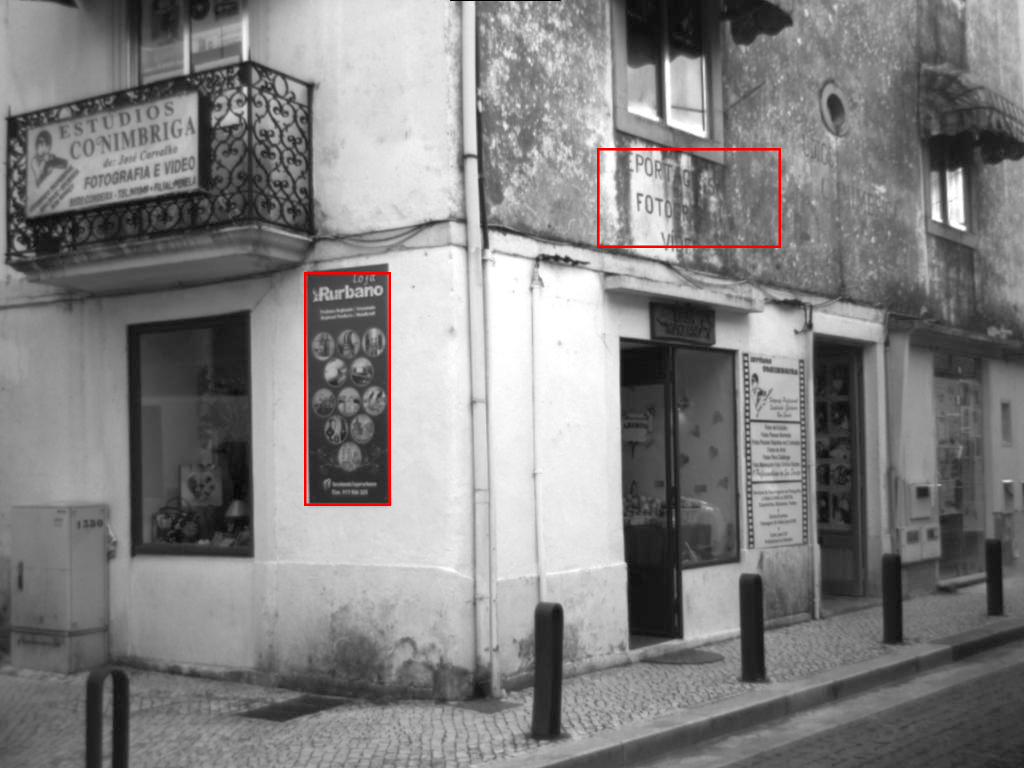
\includegraphics[width=0.80\textwidth]{./images/rectified_stereo_image/original_template_img_with_box.png}
	} \\
	\subfloat[Target image]{
		\label{fig:tar}
		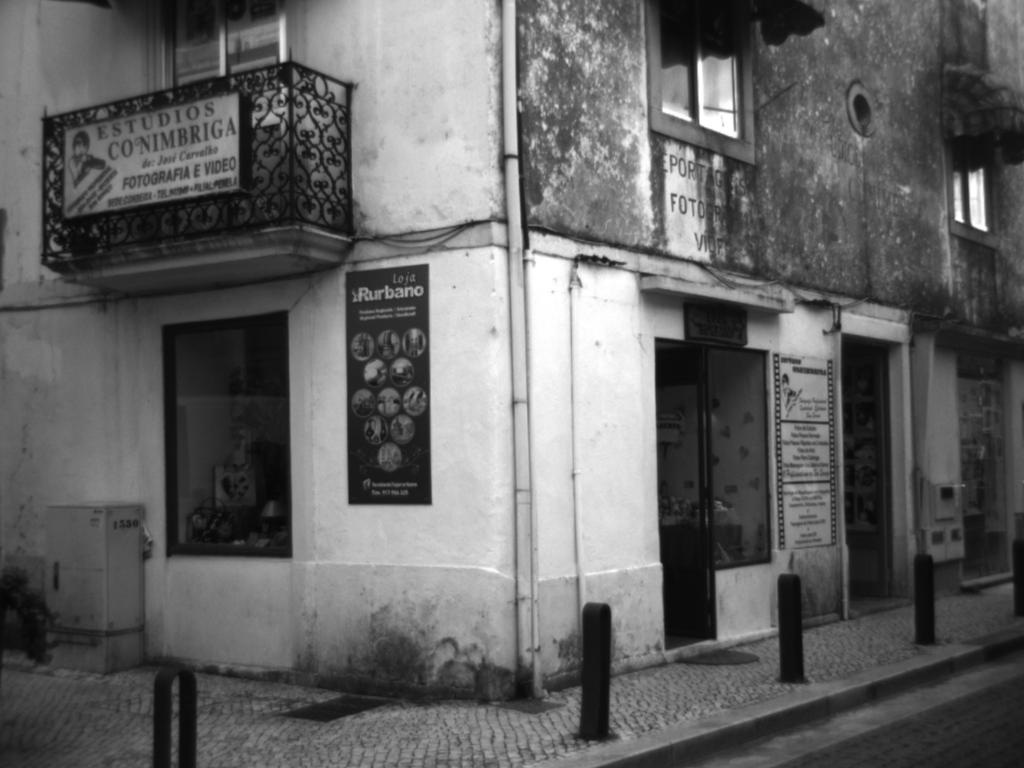
\includegraphics[width=0.80\textwidth]{./images/rectified_stereo_image/original_target_img.png}}
	\caption{Example of a rectified stereo image pair }
	\label{fig:Example rectified stereo images}
\end{figure}

Before running the program, an initialization of parameter $\vec{\beta}_n$ is needed. $a$ and $b$ will start with $1$ and $0$. The reason is that the radiometric distortion is not too much, $a$ and $b$ could start with no radiometric distortion. Parameter $\vec{q}_n$ is initialized as $(0, 0, q_{n_3})$, where $q_{n_3}$ was estimated by hand. In a future version of the algorithm this will be automated.

After initializing $\beta_n$, it is used to warp plane patch $n$ in the target image to the template image, the result of the first plane patch (billboard on the left wall) is shown in \cref{fig:billoadnleft}. Among them, \cref{fig:ddiffBill} shows the difference of this two image patches. It is built by subtract the gray value of the corresponding point. And the difference will be used as gray value of this position to build the difference image. Because the difference of most of pixels is too small, the value is re-scaled by a factor (It's 50 in the thesis) to make it more obvious. What's more, $ difference = I_2 - I_1$ and it is shown in blue for positive value and in red for negative value. 
\begin{figure}[tbp]\centering
	\subfloat[Template image ]{
				\label{fig:temBidll}
		
\includegraphics{./images/rectified_stereo_image/patch_2_ROI_of_template.png}
	} \quad
	\subfloat[Warped image]{
				\label{fig:wardpBill}
		
\includegraphics{./images/rectified_stereo_image/patch_2_ROI_of_warped_image.png}
	} \quad
	\subfloat[Difference image]{
				\label{fig:ddiffBill}
		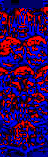
\includegraphics{./images/rectified_stereo_image/patch_2_difference.png}
	} \quad
	\subfloat[]{
		\label{fig:difadfBill}
		
\includegraphics[height = 5.5cm]{./images/legendH}
	} 
	\caption{Result of plane patch of billboard on the left wall }
	\label{fig:billoadnleft}
\end{figure}
%
%\begin{figure}[tbp]\centering
%	\subfloat[Billboard on left balcony in template image ]{
%		\label{fig:temBill}
%		
\includegraphics{./images/rectified_stereo_image/patch_1_ROI_of_template.png}
%	} \qquad
%	\subfloat[Billboard on left balcony in warped image]{
%		\label{fig:warpBill}
%		
\includegraphics{./images/rectified_stereo_image/patch_1_ROI_of_warped_image.png}
%	} \\
%	\subfloat[Difference image of billborad on left balcony]{
%		\label{fig:diffBill}
%		
\includegraphics[width = 0.4\textwidth]{./images/rectified_stereo_image/patch_1_difference.png}
%	} \\
%	\subfloat[Legend]{
%		\label{fig:Legend1}
%		
\includegraphics[width = 0.4 \textwidth]{./images/legendW}
%	} 
%	\caption{Result of plane patch of billboard on left balcony}
%	\label{fig:billonbal}
%\end{figure}
And the result of the word on right wall is shown in \cref{fig:word}

\begin{figure}[tbp]\centering
	\subfloat[Word on right wall in template image ]{
%		\label{fig:temBill}
		
\includegraphics[width = 0.5\textwidth]{./images/rectified_stereo_image/patch_3_ROI_of_template.png}
	} \\
	\subfloat[Word on right wall in warped image]{
%		\label{fig:warpBill}
		
\includegraphics[width = 0.5\textwidth]{./images/rectified_stereo_image/patch_3_ROI_of_warped_image.png}
	} \\
	\subfloat[Difference image of Word on right wall]{
%		\label{fig:diffBill}
		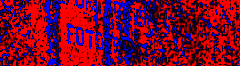
\includegraphics[width = 0.5\textwidth]{./images/rectified_stereo_image/patch_3_difference.png}
	} \\
	\subfloat[Legend]{
	%		\label{fig:diffBill}
	
\includegraphics[width = 0.5\textwidth]{./images/legendW}
	} 
	\caption{Result of plane patch of word on right wall}
	\label{fig:word}
\end{figure}

In order to quantify the accuracy of result, the definition of PSNR should be introduced here.(Here the formula of PSNR is used but it doesn't have the meaning for noise, so that the result is not an actual PSNR.)

\begin{definition}[Peak signal-to-noise ratio]\label{def:PSNR}
	Peak signal-to-noise ratio, often abbreviated \\ PSNR, is an engineering term for the ratio between the maximum possible power of a signal and the power of corrupting noise that affects the fidelity of its representation. Because many signals have a 
	very wide dynamic range, PSNR is usually expressed in terms 
	of the logarithmic decibel scale \cite{PeakSignaltonoiseRatio2020}
	
	PSNR is most easily defined via the mean squared error (MSE). Given a noise-free m×n monochrome image I and its noisy approximation K, MSE is defined as:
	\begin{align}
		\mathit{MSE} = \frac{1}{m\,n}\sum_{i=0}^{m-1}\sum_{j=0}^{n-1} [I(i,j) - K(i,j)]^2
	\end{align}
	The PSNR (in dB) is defined as:
	\begin{align}
	\mathit{PSNR} &= 10 \cdot \log_{10} \left( \frac{\mathit{MAX}_I^2}{\mathit{MSE}} \right)\nonumber \\ 
	&= 20 \cdot \log_{10} \left( \frac{\mathit{MAX}_I}{\sqrt{\mathit{MSE}}} \right)\nonumber \\ 
	&= 20 \cdot \log_{10} \left( {\mathit{MAX}_I} \right) - 10 \cdot \log_{10} \left( {{\mathit{MSE}}} \right)
	\end{align}
	Here, MAXI is the maximum possible pixel value of the image. When the pixels are represented using 8 bits per sample, this is 255.
\end{definition}

PSNR is most commonly used to measure the similarity of corresponding images. The PSNR of these three patches is shown in \cref{tab:PSNR of different patches}. The typical value for the PSNR for image registration are between $30$ and $50$ dB, provided the bit depth is $8$ bits, where higher is better. As the difference images show, the results are good, but not perfect. The reason is that the example image is not perfect rectified, so optimization of $H_\infty$ and $\rde$ is also needed, just as what is done in next section.

%And the second patch is relatively not very good, shown in the difference image, there are more deep red pixels. The probably reason is that the image is not perfect rectified, so I need to not only optimize $\vec{q}_n$ but also optimize $H_\infty$ and $\rde$. What's more, there are much noise in the original image, in order to reduce the impact of noise, I also blur the image. The implementation result with optimization is shown in \cref{fig:Result of plane patch of word on billboard on left balcony after optimization}.

%\begin{figure}[tbp]\centering
%	\subfloat[Billboard on left balcony in template image]{
%		%		\label{fig:temBill}
%		
\includegraphics[width = 0.4\textwidth]{./images/rectified_stereo_image/patch_1_of_cycle_6_ROI_of_template}
%	} 
%	\subfloat[Billboard on left balcony in warped image ]{
%		%		\label{fig:warpBill}
%		
\includegraphics[width = 0.4\textwidth]{./images/patch_1_of_cycle_6_ROI_of_warped_image}
%	} 
%	\caption{Result of plane patch of word on billboard on left balcony after optimization $H_\infty$ and $\rde$}
%	\label{fig:Result of plane patch of word on billboard on left balcony after optimization}
%\end{figure}

\begin{table}[tbp]
	\centering
	\scriptsize  
	\begin{tabular}{p{120pt} p{60pt}}
		\toprule
		Patch & {\bfseries PSNR(dB)}\\ \midrule
		 Billboard on the left wall  &  35.8293\\
		\addlinespace[3pt]
		Word on right wall & 32.0190 \\ \bottomrule
	\end{tabular}
	\caption{PSNR of different patches for rectified images}  
	\label{tab:PSNR of different patches} 
\end{table}

\subsection{Unrectified Images}\label{subsec:Unrectified Images}
Research is extended from special cases to general cases. In last section, the result of the algorithm on rectified stereo images is shown. Next, the algorithm will be applied to normal case, unrectified images, which appears more often in the practical applications. There is no special parameters for normal case, so the whole iterative process shown in \cref{fig:optimized iterative process} will be implemented. The process is divided into two parts: Optimize $\vec{Q}^k, \vec{R}^k$ per patch separately with constant $H_\infty^{(k)}, \rde^{(k)}$ and Optimize $H_\infty^{(k)}, \rde^{(k)}$ for all patches with constant $\vec{Q}^{(k)}, \vec{R}^{(k)}$, where $\vec{Q}^{(k)} = (\vec{q}_1^T, \vec{q}_2^T, \cdots, \vec{q}_n^T)^T$ and $\vec{R}^{(k)}= (\vec{r}_1^T, \vec{r}_2^T, \cdots, \vec{r}_n^T)^T$ with $\vec{r}_n^T= ({r_n}_1, {r_n}_2)$. The first steps Optimize $\vec{Q}^k, \vec{R}^{(k)}$  will be done just like the process in \cref{subsec:Rectified Stereo Images}, the only difference is that $H_\infty^k$ and $\rde^k$ are not always $I_3$ and $(1, 0, 0)^T$ but result of the last iterative process $H_\infty^{k}, \rde^k$. 

So in this section, we will mainly discuss the second part. Detailed calculation process for the second part is shown next. After the step Optimize $\vec{Q}^k, \vec{R}^{(k)}$, the $\vec{q}_n^T$ and $\vec{r}_n^T$ for all patches are got and can be regarded as constant values in this step. So there are only parameter $H_\infty$ and $\rde$ to be optimized. The $\vec{\beta}$ (\cref{eq:beta}) becomes 
\begin{align}
	\vec{\beta} =  \begin{pmatrix}\operatorname {vec}(H_\infty)\\\rde\end{pmatrix}
\end{align}
the Jacobian matrix $\mathbf{J}_{F_n}$ for patch n: 
\begin{align}
	\mathbf{J}_{F_n} = \begin{pmatrix}
	\frac{\mathrm{d} I_2(N)}{\mathrm{d}N} \cdot \frac{\mathrm{d} N(T_n)}{\mathrm{d} T_n} \cdot \frac{\partial T_n(H_\infty, \rde, \rdx_{11})}{\partial \operatorname {vec}(H_\infty)} & \frac{\mathrm{d} I_2(N)}{\mathrm{d}N} \cdot \frac{\mathrm{d} N(T_n)}{\mathrm{d} T_n} \cdot \frac{\partial T_n(H_\infty, \rde, \rdx_{11})}{\partial \rde} \\
	\frac{\mathrm{d} I_2(N)}{\mathrm{d}N} \cdot \frac{\mathrm{d} N(T_n)}{\mathrm{d} T_n} \cdot \frac{\partial T_n(H_\infty, \rde, \rdx_{12})}{\partial \operatorname {vec}(H_\infty)} & \frac{\mathrm{d} I_2(N)}{\mathrm{d}N} \cdot \frac{\mathrm{d} N(T_n)}{\mathrm{d} T_n} \cdot \frac{\partial T_n(H_\infty, \rde, \rdx_{12})}{\partial \rde} \\
	\vdots & \vdots \\
	\frac{\mathrm{d} I_2(N)}{\mathrm{d}N} \cdot \frac{\mathrm{d} N(T_n)}{\mathrm{d} T_n} \cdot \frac{\partial T_n(H_\infty, \rde, \rdx_{ij})}{\partial \operatorname {vec}(H_\infty)} & \frac{\mathrm{d} I_2(N)}{\mathrm{d}N} \cdot \frac{\mathrm{d} N(T_n)}{\mathrm{d} T_n} \cdot \frac{\partial T_n(H_\infty, \rde, \rdx_{ij})}{\partial \rde} \\
	\end{pmatrix}
\end{align}
where $\rdx_{ij} = (\rdx'_{ij}, 1)^T$ and $\rdx_{ij}$ means the $i$ row $j$ column in every patch. They are not the same for different patches. Combine all $\mathbf{J}_{F_n}$, the total $\mathbf{J}_{F}$ is
\begin{align}\label{eq:J_F}
	\mathbf{J}_{F} = \begin{pmatrix} \mathbf{J}_{F_1}\\
	\mathbf{J}_{F_2}\\
	\vdots\\
	\mathbf{J}_{F_n} 
	\end{pmatrix}
\end{align}
The total $\mathbf{J}_{F}$ matrix can be calculated explicit by bringing $\frac{\mathrm{d} N(T_n)}{\mathrm{d} T_n}$ (\cref{eq:n}), $\frac{\partial T_n(H_\infty, \rde, \rdx_{ij})}{\partial \operatorname {vec}(H_\infty)}$ (\cref{eq:H_infty2}) and $ \frac{\partial T_n(H_\infty, \rde, \rdx_{ij})}{\partial \rde}$ (\cref{eq:e1}) into the equation above.

The next step is calculating the total mapping error $\vec{E}$. Just like mentioned in \cref{subsec:Rectified Stereo Images} (\cref{eq:e_n2}), the mapping error $\vec{e}_n$ can be expressed as
\begin{align}
\vec{e}_{n} = \begin{pmatrix} 
	R_n(I_1(N(\rdx_{11})))-F_n(H_\infty, \rde, \rdx_{11})\\
	R_n(I_1(N(\rdx_{12})))-F_n(H_\infty, \rde, \rdx_{12})\\
	\vdots\\
	R_n(I_1(N(\rdx_{ij})))-F_n(H_\infty, \rde, \rdx_{ij})
\end{pmatrix}
\end{align}
Put all $\vec{e}_{n}$ together in $\vec{E}$:
\begin{align}
	\vec{E} = \begin{pmatrix} 
	\vec{e}_{1}\\
	\vec{e}_{2}\\
	\vdots\\
	\vec{e}_{n}
	\end{pmatrix}
\end{align}

Finally $\vec{\beta}$ is iteratively optimized by 
\begin{align}
	\vec{\beta}^{(k+1)} = \vec{\beta}^{(k)} + \left(\mathbf{J}_{F}^{T} \mathbf{J}_{F} \right)^{-1} \mathbf{J}_{F}^{T} \vec{E}
\end{align}

The next step is to implement the algorithm in Python and apply it to example unrectified stereo images. The algorithm will be evaluated on synthetic test images for which the ground truth is available. The details are shown in \cref{sec:Self-Built Datasets}. The template image $I_1$ and target image $I_2$ are shown in \cref{fig:Example unrectified images}. There are three planes in the image, which show a deer, a bouquet of flowers and a cat. Therefore I simply call them deer plane, flower plan and cat plane. 

\begin{figure}[htbp]\centering
	\subfloat[Template image]{
		\label{fig:tem_un}
		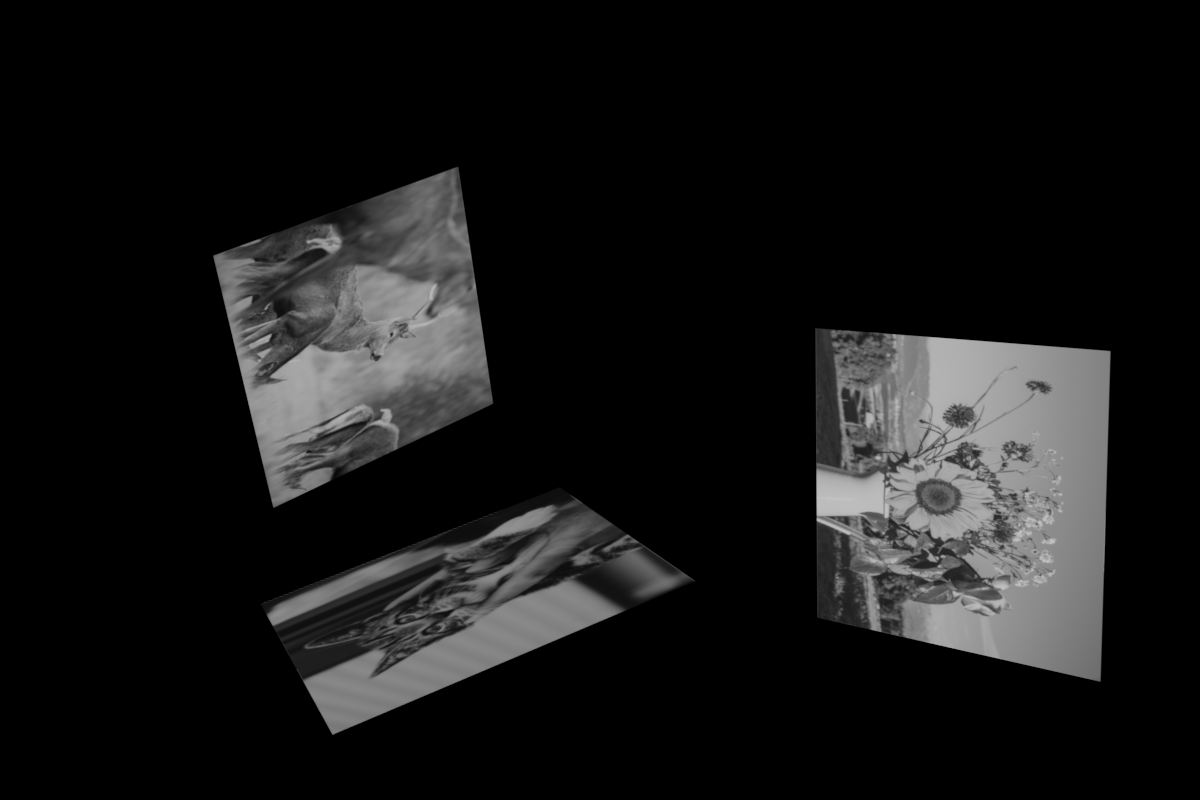
\includegraphics[width=0.80\textwidth]{./images/unrectified_images/original_template_img}
	} \\
	\subfloat[Target image]{
		\label{fig:tar_un}
		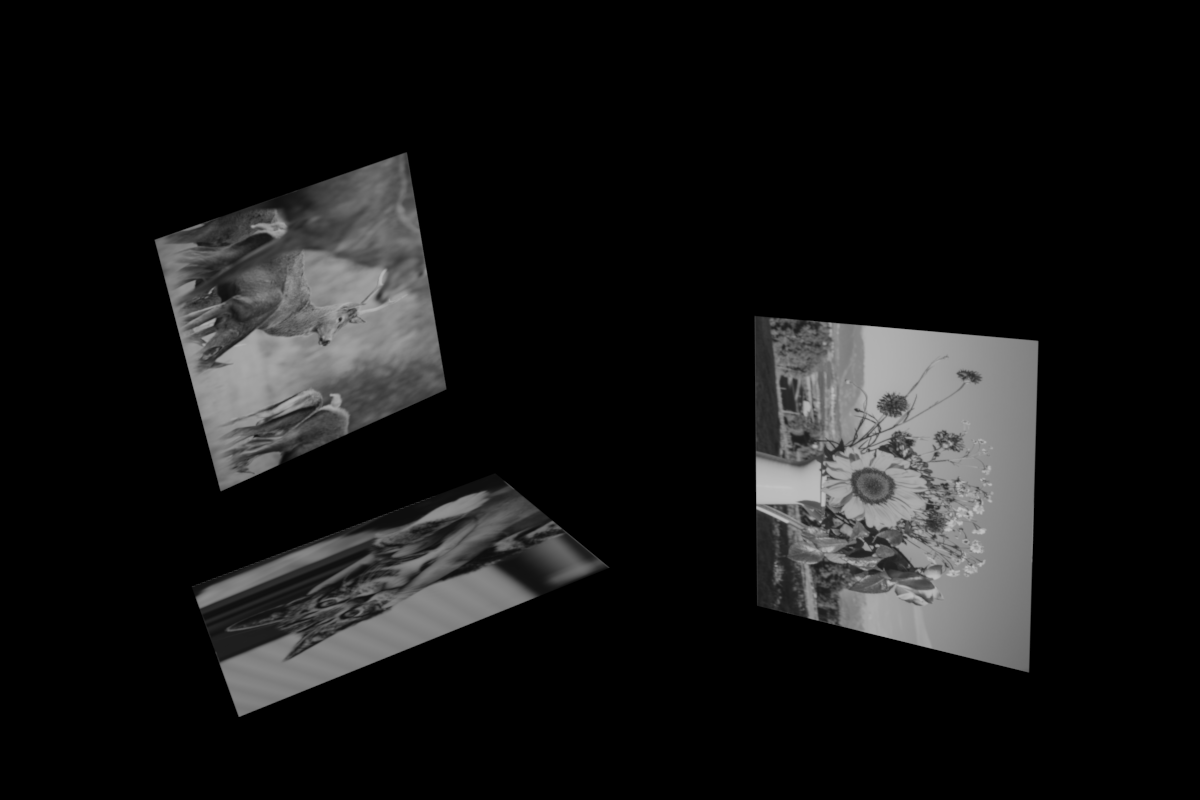
\includegraphics[width=0.80\textwidth]{./images/unrectified_images/original_target_img}}
	\caption{Example unrectified images}
	\label{fig:Example unrectified images}
\end{figure}

Because the testing image pair is synthetically generated, the ground truth is available as well. I will use them to have a good initialization of parameters $H_\infty$, $\rde$ and $\vec{Q}$, which could also be got with the GPS and INS information or EXIF data in practical application.

Just like what is done for rectified stereo images, the final result $H_\infty$, $\rde$, $\vec{Q}$ and $R$ are used to warp the target image to the template image shown in \cref{fig:Result of Unrectified Images}. And the PSNR is shown in \cref{tab:PSNR of different patches in unrectified images}. In order to evaluate the result of the proposed algorithm, the root mean squared displacement (RMSD) is introduced here. 

\begin{definition}[Root mean squared displacement]\label{def:RMSD}
	Because we know the ground truth (homography matrices of different regions of interest ${H_n}_{gt}$) of the self-built image pairs. The ground truth target ${\rdy'_{ij}}_{gt}= N({H_n}_{gt} \cdot \rdx_{ij})$ can be calculated. Then the position $\rdy'_{ij}$ of warped point can be calculated with the estimated homography matrices $H_n$:
	\begin{align}
		\rdy'_{ij} = N(H_n \cdot \rdx_{ij})
	\end{align}

	Root mean squared displacement (RMSD) is defined as
	\begin{align}
	\mathrm{RMSD} & = \sqrt{\frac{1}{n}\sum_{\rdx_{ij}\in ROI} \|\rdy'_{ij} - {\rdy'_{ij}}_{gt} \|^2}
	\end{align}
	where $n$ means the number of points in the region of interest (patches) and $\|\rdy'_{ij} - {\rdy'_{ij}}_{gt} \|$ is the distance $d$ between tow points. RMSD is the measure of the average distance between two vector space, here means how much the difference between the estimated result and ground truth.
\end{definition}
	
The root mean squared displacement (RMSD) and maximum displacement of all patches are shown in \cref{tab:Displacement of different patches for unrectified images}. From the difference images, we can see visually that there is basically no difference. From the PSNR analysis, the value is relatively high. So the result is acceptable. And because the whole parameters are optimized, there are no large matching error as in the rectified case (\cref{fig:word})
\begin{figure}[htbp]\centering
	\subfloat[Template image]{
		\label{fig:Template Image1}
		
\includegraphics[width=0.30\textwidth]{images/unrectified_images/patch_1_of_cycle_1_ROI_of_template}
	}  \hspace{-2mm}
	\subfloat[Warped image for deer plane]{
		\label{fig:Warped Image For Deer Plane}
		
\includegraphics[width=0.30\textwidth]{images/unrectified_images/patch_1_of_cycle_1_ROI_of_warped_image}
	} \hspace{-2mm}
	\subfloat[Difference image]{
		\label{fig:Difference Image1}
		
\includegraphics[width=0.30\textwidth]{images/unrectified_images/patch_1_difference}
	}\hspace{-2.5mm}
	\subfloat[]{
	%		\label{fig:diffBill}
	
\includegraphics[height = 3.6cm]{./images/legendH}
	} 
	\\

	\subfloat[Template image]{
		\label{fig:Template Image2}
		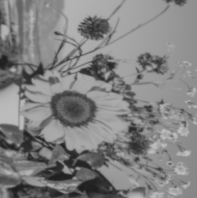
\includegraphics[width=0.30\textwidth]{images/unrectified_images/patch_2_of_cycle_1_ROI_of_template}
	} \hspace{-2mm}
	\subfloat[Warped image for flower plane]{
		\label{fig:Warped Image For Flower Plane}
		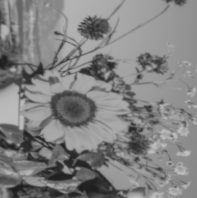
\includegraphics[width=0.30\textwidth]{images/unrectified_images/patch_2_of_cycle_1_ROI_of_warped_image}
	}\hspace{-2mm}
	\subfloat[Difference image]{
		\label{fig:Difference Image2}
		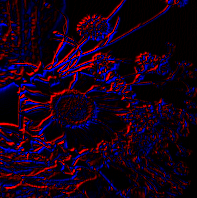
\includegraphics[width=0.30\textwidth]{images/unrectified_images/patch_2_difference}
	}\hspace{-2.5mm}
	\subfloat[]{
	%		\label{fig:diffBill}
	
\includegraphics[height = 4.3cm]{./images/legendH}
} 
	\\

	\subfloat[Template image]{
		\label{fig:Template Image3}
		
\includegraphics[width=0.30\textwidth]{images/unrectified_images/patch_3_of_cycle_1_ROI_of_template}
	} \hspace{-2mm}
	\subfloat[Warped image for cat plane]{
		\label{fig:Warped Image For Cat Plane}
		
\includegraphics[width=0.30\textwidth]{images/unrectified_images/patch_3_of_cycle_1_ROI_of_warped_image}
	} \hspace{-2mm}
		\subfloat[Difference image]{
		\label{fig:Difference Image3}
		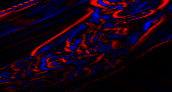
\includegraphics[width=0.30\textwidth]{images/unrectified_images/patch_3_difference}
	}\hspace{-2.5mm}
	\subfloat[]{
	%		\label{fig:diffBill}
	
\includegraphics[height = 2.4cm]{./images/legendH}
} 
\\
	\caption{Result of unrectified Images}
	\label{fig:Result of Unrectified Images}
\end{figure}

\begin{table}[htbp]
	\centering
	\scriptsize  
	\begin{tabular}{p{80pt} p{60pt}}
		\toprule
		Patch & {\bfseries PSNR(dB)}\\ \midrule
		Deer Plane&  44.9857\\
		\addlinespace[3pt]
		Flower Plane  &  38.3061\\
		\addlinespace[3pt]
		Cat Plane & 41.5518 \\ \bottomrule
	\end{tabular}
	\caption{PSNR of different patches for unrectified images}  
	\label{tab:PSNR of different patches in unrectified images} 
\end{table}

\begin{table}[htbp]
	\centering
	\scriptsize   
	\begin{tabular}{p{80pt} p{60pt} p{60pt}}
		\toprule
		 Patch & {\bfseries RMSD (pixel)} & {\bfseries Maximum(pixel)}\\ \midrule
		 Deer Plane&  0.186577&0.370456 \\
		 \addlinespace[3pt]
		 Flower Plane  &  0.130046&0.162404 \\
		 \addlinespace[3pt]
		 Cat Plane & 0.369888&0.874363 \\ 
		 \addlinespace[3pt]
		 All Patches & 0.215594&0.874363 \\ \bottomrule
	\end{tabular}
	\caption{Displacement of different patches for unrectified images}  
	\label{tab:Displacement of different patches for unrectified images} 
\end{table}
In this chapter I only show one example result of the algorithm for each case. More results are listed evaluation in \cref{ch:Evaluation}.









\section{Program}\label{sec:Program}
In this section, I mainly introduce the methods and theories related to programming.  For example, during programming, the library OpenCV is used, but some basic information, like which kind of coordinate it uses for function "warpPerspective", is not included in the documentation of it. So I had to figure them out. What's more,  how to blur images and calculate image derivatives are also mentioned here.  In the end, dyadic program is introduced. 

\subsection{Image Warping}\label{subsec:Image Warping}
In order to do image registration, the function to warp image is needed. In the thesis, I have chosen the library OpenCV for warping images. How to warp the target image to the template image with the calculated homography matrix is a very important step of implementation.

Because homography is a perspective transformation, OpenCV calls the function "warpPerspective" to warp an image with a homography matrix. The function applies a perspective transformation to an image. The introduction of it in OpenCV documentation \cite{opencvdevteamOpenCV13Documentation} is listed here:
\begin{python}[caption={Model of warpPerspective},label={lst:model of warpPerspective}]
	cv2.warpPerspective(src, M, dsize[, dst[, flags[, borderMode[, borderValue]]]])
\end{python}
where
the parameters: 
\begin{itemize}
	\item \textbf{src} - input image
	\item \textbf{M} - $3 \times 3$ homography transformation matrix
	\item \textbf{dsize} - size of the output matrix
	\item \textbf{flags} - combination of interpolation methods(INTER\_LINEAR or INTER\_NEAREST) and the optional flag WARP\_INVERSE\_MAP, that sets $M$ as the inverse transformation ($ dst \rightarrow src $)
	\item \textbf{borderMode} - piexl extrapolation 
	methode (BORDER\_CONSTANT \\ or BORDER\_REPLICATE).
	\item \textbf{borderValue} - value used in case of a constant border; by default, it equals 0.
\end{itemize}
The function transforms the source image using the specified matrix:
\begin{align}
	dst(x, y) = src\left( \frac{M_{11}x + M_{12}y+ M_{13}}{M_{31}x+M_{32}y + M_{33}}, \frac{M_{21}x + M_{22}y + M_{23}}{M_{31}x + M_{31}y + M_{33}} \right)
\end{align}
when the flag "	WARP\_INVERSE\_MAP" in the function is set, Otherwise, the transformation is first inverted with \textbf{invert()} and then put in the formula above instead of \textbf{M}. 

According to this, the target image $I_2$ is put into the function "warpPerspective" as \textbf{src}. And $H_{n} = H_{\infty} + \vec{e} \cdot \vec{q}_{n}^T$ is set as \textbf{M}. And the \textbf{flags} are INTER\_LINEAR and WARP\_INVERSE\_MAP. The output of the function is a warped image which is used to show the estimation result and compare with the template image $I_1$ to get the mapping error $\vec{e}_n$. 

But what we optimize in the program are $H_{\infty}$,  $\vec{e}$ and $ \vec{q}_{n}^T$. There isn't explicit homography matrix $H_n$ in program. In order to warp the image with $H_{\infty}$,  $\vec{e}$ and $ \vec{q}_{n}^T$, a new function based on "warpPerspective" is built to warp the image in the program:
\begin{python}[caption={warp\_image},label={lst:warpimage}]
	def warp_image(q, e, H_inf, target_img, template_img):
		H = H_inf + e @ q.T
		
		width_x = np.array(template_img).shape[1]
		height_y = np.array(template_img).shape[0]
		
		warped_img = cv2.warpPerspective(target_img, H, (width_x, height_y),
		flags=cv2.INTER_LINEAR + cv2.WARP_INVERSE_MAP)
	return warped_img
\end{python}

Although the openCV documentation describes the parameters of functions in detail, the specific description of the coordinate system is not involved. For example, the specific location of the origin, the direction of the coordinate axis, and how to perform homogeneous and dehomogeneous are not clearly indicated. But for image registration technology, accuracy is very important. Therefore, the above problems need to be explored and the program must be adjusted accordingly to ensure accuracy.

First tests with the function reveal that x-axis points right, y-axis points downwards and z-axis for homogenization and dehomogenization of the homogeneous coordinates. But it can be only seen that the origin of pixel coordinate is somewhere on the top left corner. There are two types of pixel coordinate. 
\begin{enumerate}
	\item The origin is at the middle of the upper left corner pixel of the image with the positive Row axis pointing downwards and the positive Column axis pointing towards the right \cite{misbPhotogrammetryMetadataSet}.
	\item The origin is at the upper left corner of the upper left pixel of the image with the positive Line axis pointing downwards and the positive Column axis pointing towards the right \cite{misbPhotogrammetryMetadataSet}.
\end{enumerate}

To clarify this problem, a little test program is used. Assumed that a simple image (shown in \cref{fig:Test Image}) with only 4 pixel, which is 
\begin{align}
\begin{bmatrix}
100&170\\
170&170 
\end{bmatrix} \nonumber
\end{align}
is transformed by a homography matrix
\begin{align}
\begin{bmatrix}
2&0&0\\
0&2&0\\
0&0&1\\
\end{bmatrix} \nonumber
\end{align}
which is corresponds to scale the template image by factor $2$.(In function "warpPerspective", \textbf{flag} WARP\_INVERSE\_MAP is not used in the test.) And if the gray value of a quarter area in the upper left corner in the warped image is $100$, this proves that the origin is at the upper left corner of the upper left pixel of the image in the function "warpPerspective". Otherwise, the type 1 is used. 

The result should is shown in \cref{fig:Result Image}. It's obvious from the result, that the function regards the middle of pixel at upper left corner as the origin of the pixel coordinate. So I will use this definition in the thesis, too.
\begin{figure}[htbp]\centering
	\subfloat[Testing image]{
		\label{fig:Test Image}
		
\includegraphics[width=0.20\textwidth]{images/tofindorigin/img_2_transform.png}
	} \qquad
	\subfloat[Result image]{
		\label{fig:Result Image}
		
\includegraphics[width=0.40\textwidth]{images/tofindorigin/img_form.png}
	} 
	\caption{Origin of the coordinate system used by "warpPerspective"}
	\label{fig:Searching Origin}
\end{figure}

\subsection{Image Pyramid}
In cases, images contain much noise. In image processing, it will influence the result. So before implementation of the algorithm, we must reduce the noise in image. There are some low pass filters, which can be used for image blurring. Here I have chosen the most common filter, Gaussian filter to make a Gaussian blur. In addition, it's also used in the thesis to make a Gaussian pyramid of images to reduce the effects of repeating structure and allow for a large range of convergence of the algorithm.

The proposed algorithm is based on the least square method. Therefore, the less blurry the image, the more noise will be introduced into the iterative process, and the greater the interference to the final result. At the same time, the algorithm will converge slowly because of noise influence. To avoid this problem, image pyramid is used in the program.

Go further, when there is repeating structures (texture) in the target plane such as brick floor, the repetitive structure can be almost blurred away with image pyramid and there is enough other structure left that make the algorithm converge.

In the program, the function "pyrDown" from OpenCV is used to build  Gaussian image pyramid(An example image pyramid built by this function is shown in \cref{fig:iamge pyramid}).
\begin{python}[caption={Image pyramid}, label={lst:Imagepyramid}]
	cv2.pyrDown(src[, dst[, dstsize[, borderType]]])
\end{python}
With this function, an image pyramid as a set of layers in which the higher the layer, the smaller the size is build.

After building an image pyramid of testing image, the algorithm will first calculate at the highest layer of the pyramid, which is the layer with the lowest resolution. When the preliminary result is obtained, it will be re-scaled into next layer and used as the initialization of next layer. With this initialization, the algorithm runs on the next layer. Repeat this until the last layer or the original image. Then the result has no offset and more accurate. At the same time the algorithm converges faster. Because it takes less time to converge, when the algorithm is applied to the lower resolution image. With a prior result for initialization of the higher resolution image, it also reduces the running time of the algorithm.

\begin{figure}[htbp]\centering
	\subfloat[Image in 3rd layer]{
	
		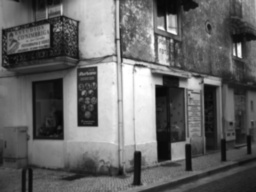
\includegraphics[width = 2cm]{./images/ImagePyramid/template_img_pyramid_of2_layer}
	} \\
	\subfloat[Image in 2nd layer]{

		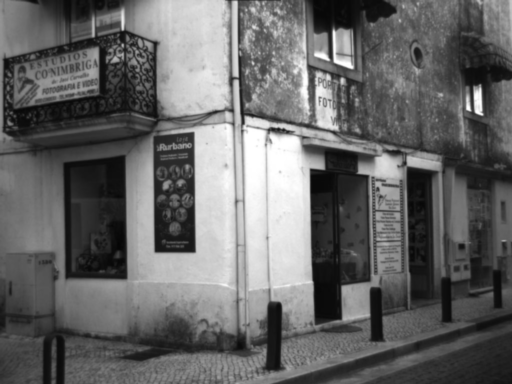
\includegraphics[width = 4cm]{./images/ImagePyramid/template_img_pyramid_of1_layer}
	} \\
	\subfloat[Image in 1st layer]{

	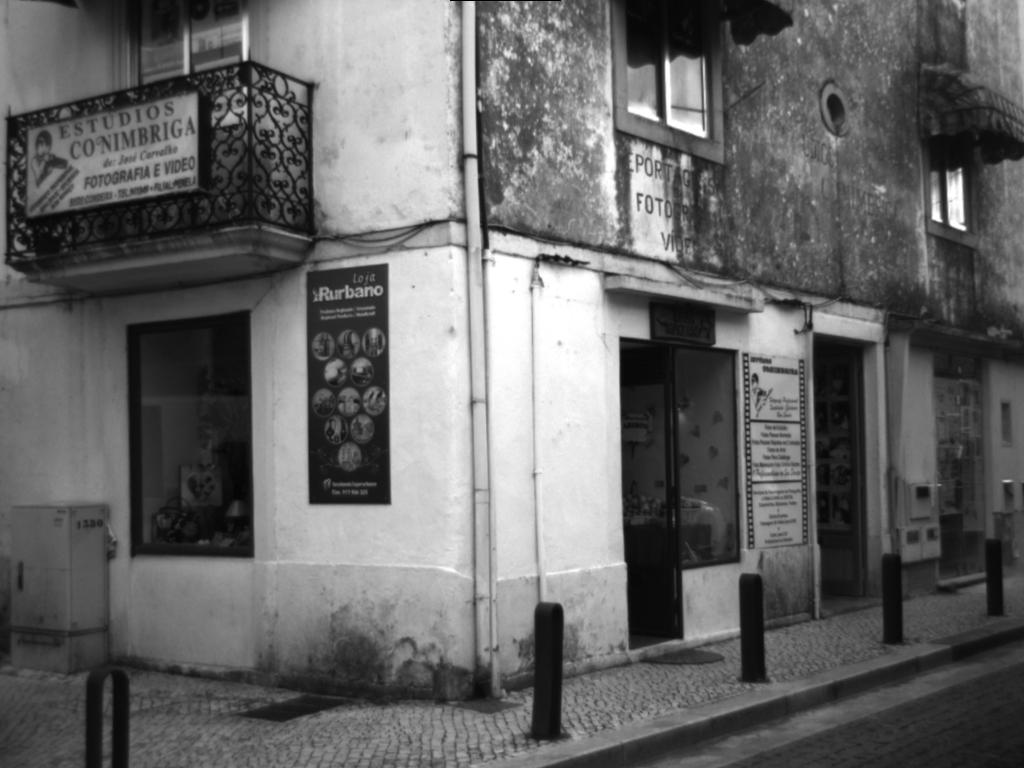
\includegraphics[width = 8cm]{./images/ImagePyramid/template_img_pyramid_of0_layer}
	} 
	\caption{Visual representation of an image pyramid with 3 levels}
	\label{fig:iamge pyramid}
\end{figure}



\subsection{Image Derivatives}\label{sec:Image derivatives}
When talking about the derivative of an image, you're actually talking about what's called a discrete derivative, and it's more of an approximation of the derivative. One simple example is that you can take the derivative in the x-direction at pixel $\rdx'_{ij}$ by taking the difference between the pixel values to the left and right of your pixel. It's widely used in edge detection. But in my thesis, only the first derivation of image is needed to approximate the term $\frac{\mathrm{d} I_2(N)}{\mathrm{d}N}$ in \cref{eq:jnuR}:
\begin{align}
	j_{nu} 
	= \frac{\mathrm{d} I_2(N)}{\mathrm{d}N} \frac{\mathrm{d} N(T_n)}{\mathrm{d} T_n} \frac{\partial T_n(\vec{\beta}, \rdx_{ij})}{\partial \beta_u} \nonumber
\end{align}

In computer version, image derivatives can be computed by using small convolution filters of size $2 \times 2$ or $3 \times 3$, such as Sobel, Roberts and Prewitt operators. However, a large mask will generally give a better approximation of the derivative and examples of such filters are Gaussian derivatives and Gabor filters. Sometimes high frequency noise needs to be removed and this can be incorporated in the filter so that the Gaussian kernel will act as a band pass filter in the process. The most used derivatives filter kernel is shown in \cref{fig:Derivative Filter}.
\begin{figure}[htbp]
	\centering
	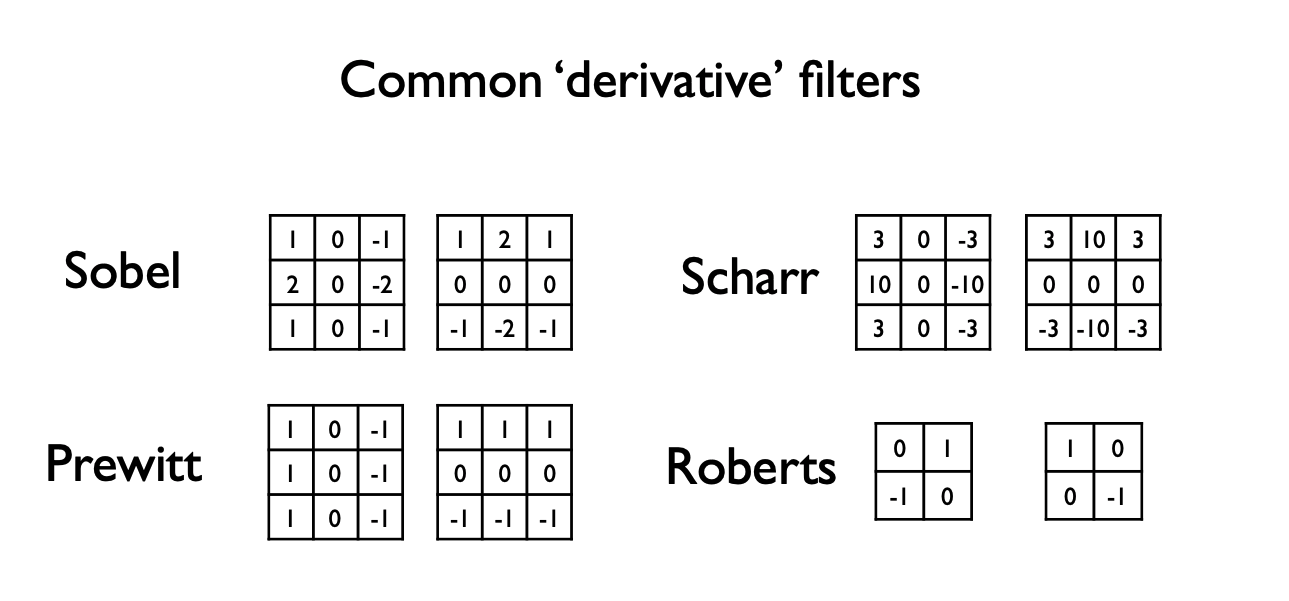
\includegraphics[width=0.80\textwidth]{images/derivatives}
	\caption{Derivative filter}
	\label{fig:Derivative Filter}
\end{figure}

In the Library OpenCV, there is a function "cv2.Sobel" to calculate the first, second, third or mixed derivatives using extended Sobel operator. This is used to calculate the image derivatives in the implementation. 

The Sobel operator uses two $3\times3$ kernel (usually) which are convolved with the original image to calculate approximations of the derivatives - one for horizontal changes, and one for vertical. If we define $A$ as the source image, and $G_x$ and $G_y$ are two images which at each point contain the vertical and horizontal derivative approximations respectively, the computations are as follows \cite{SobelOperator2020}:
\begin{align}
	G_x = \frac{1}{8}\begin{bmatrix} 
		+1 & 0 & -1  \\
		+2 & 0 & -2 \\
		+1 & 0 & -1 
	\end{bmatrix} * A
	\quad
	\mbox{and}
	\quad   
	G_y = \frac{1}{8}\begin{bmatrix} 
		+1 & +2 & +1\\
		0 & 0 & 0 \\
		-1 & -2 & -1
	\end{bmatrix} * A
\end{align}
where $*$ here denotes the 2-dimensional signal processing convolution operation.

The function "cv2.Sobel" in OpenCV \cite{opencvdevteamOpenCV13Documentation}shows:
\begin{python}[caption={Model of Sobel Filter},label={lst:Model of Sobel filter}]
	cv2.Sobel(src, ddepth, dx, dy[, dst[, ksize[, scale[, delta[, borderType]]]]]) 
\end{python}

However, the Sobel operator, while reducing artifacts associated with a pure central differences operator, does not have perfect rotational symmetry.  Scharr looked into optimizing this property. Scharr operators result from an optimization minimizing weighted mean squared angular error in Fourier domain. This optimization is done under the condition that resulting filters are numerically consistent. Therefore, they really are derivative kernels rather than merely keeping symmetry constraints \cite{SobelOperator2020}.

There is also a special value $ksize=CV\_SCHARR(-1)$ of function "cv2.Sobel" that corresponds to the $3\times3$ Scharr filter in function that gives more accurate results than the Soble operator. The Scharr aperture is:
\begin{align}
	\frac{1}{32}\begin{bmatrix}
		-3& 0& 3\\
		-10&0&10\\
		-3&0&3
	\end{bmatrix} \nonumber
\end{align}
for the x-derivative, or transposed for the y-derivative.

The function combine Gaussian smoothing and differentiation, so the result is more or less resistant to the noise. Most often, the function is called with (xorder =1, yorder =0) or (xorder =0, yorder =1) to calculate the first x- or y- image derivative.

In the thesis, what needed in program is $\frac{\mathrm{d} I_2(N)}{\mathrm{d}N} $, with
\begin{align}
		\rdy'_{ij} &= N(\rdy_{ij}) \nonumber \\
		\rdy_{ij} & = (H_{\infty} + \rde \cdot \vec{q}_{n}^T) \rdx_{ij} \nonumber 
\end{align}
The meaning of this term is the derivative of pixel $\rdy'_{ij}$ in image $I_2$. To get this, the exact $\rdy'_{ij}$ corresponding to $\rdx'_{ij}$ should be known. So the function "warp\_image" in \cref{subsec:Image Warping} combining function "cv2.Sobel" can complete this task.  Function "warp\_image" calculates $\rdy'_{ij}$ and function "cv2.Sobel" calculates the derivative. An example is shown below:
\begin{enumerate}
	\item First, use function "cv2.Sobel" function to calculate the first x and y derivative of origin image $I_2$:
\begin{python}[caption={Derivative in x and y direction},label={lst:Model of Sobel Fildaster}]
	ImageDerivativeX = cv2.Sobel(target_img, -1, 1, 0, ksize=-1)
	ImageDerivativeY = cv2.Sobel(target_img, -1, 0, 1, ksize=-1)
\end{python}
\item Then the output of last step should be warped with function "warp\_image" and $H_{\infty}$,  $\vec{e}$ and $ \vec{q}_{n}^T$:
\begin{python}[caption={$\frac{\mathrm{d} I_2(N)}{\mathrm{d}N} $},label={lst:Model of Sdasobel Fildaster}]
	ImageDerivativeX_warp = self.warp_image(q, e, H_inf, ImageDerivativeX, template_img)
	ImageDerivativeY_warp = self.warp_image(q, e, H_inf, ImageDerivativeY, template_img)
\end{python}
\end{enumerate}

\subsection{Dyadic Program}\label{Dyadic Program}
Generally speaking, the images that are the objects of our algorithm contain all millions to ten of millions pixels. So when I apply the algorithm, the dimension of  \cref{eq:J_F} will reach 20 million even more. In this way, when we calculate pseudo-inverse of $\mathbf{J}_{F}$, it will require a very large memory space and running time, which greatly increases the computation time of algorithm. In order to avoid this problem, I will optimize it during programming, so as to improve the reaction speed of the program.

The main idea is to use dyadic product to build a dyadic program. In mathematics, specifically multilinera algebra, a dyadic or dyadic tensor is a second order tensor, written in a notation that fists in with vector algebra. The dyadic product takes in two vectors and returns a second order tensor called a "dyadic". A dyadic can be used to contain physical or geometric information, although in general there is no direct way of geometrically interpreting it.

It also has some aspects of matrix algebra, as the numerical components of vector can be arranged into row and column vectors, and those of second order tensors in square matrix. Dyadic expressions may closely resemble the matrix equivalents.

Here I will use the process of calculating \cref{eq:simple} in step Optimize $\vec{Q}^k, \vec{R}^k$ per patch to explain the details of using dyadic product. In each cycle, the term
\begin{align}
	\left(\mathbf{J}_{F_n+R_n}^{T} \mathbf{J}_{F_n+R_n} \right)^{-1} \mathbf{J}_{F_n+R_n}^{T} \vec{e}_{n} \nonumber
\end{align} 
should be calculated. Rewrite $\mathbf{J_{F_n+R_n}}$ in this form:
\begin{align}
	\mathbf{J_{F_n+R_n}} = \begin{pmatrix}
		B_1^T\\
		B_2^T\\
		\vdots\\
		B_{i\times j}^T
		\end{pmatrix}
\end{align}
where 
\begin{align}
	B_{i \times j}^T &= \begin{pmatrix}\frac{\mathrm{d} I_2(N)}{\mathrm{d}N}\cdot \frac{\mathrm{d} N(T_n)}{\mathrm{d} T_n}\cdot \frac{\partial T_n(\vec{q}_n, \rdx_{ij})}{\partial \vec{q}_n}&- \frac{\partial R_n(I_1(N(\rdx_{ij})))}{\partial {r_1}_n} & - \frac{\partial R_n(I_1(N(\rdx_{ij})))}{\partial {r_2}_n} \end{pmatrix}\\
	&= \begin{pmatrix} b_{i \times j}^{(1)} & b_{i \times j}^{(2)} & b_{i \times j}^{(3)}\end{pmatrix}
\end{align}
with 
\begin{align}
b_{i \times j}^{(1)} &= \frac{\mathrm{d} I_2(N)}{\mathrm{d}N}\cdot \frac{\mathrm{d} N(T_n)}{\mathrm{d} T_n}\cdot \frac{\partial T_n(\vec{q}_n, \rdx_{ij})}{\partial \vec{q}_n} \nonumber \\
b_{i \times j}^{(2)} & = - \frac{\partial R_n(I_1(N(\rdx_{ij})))}{\partial {r_1}_n} \nonumber \\
b_{i \times j}^{(3)}&= - \frac{\partial R_n(I_1(N(\rdx_{ij})))}{\partial {r_2}_n} \nonumber 
\end{align}
and $b_{i \times j}^{(1)}$ is a $1 \times 3$ vector, $b_{i \times j}^{(2)}$ and $b_{i \times j}^{(3)}$ are both scalar each. So the dimension of $B_{i \times j}^T $ is $1 \times 5 $ in this case

So the term $\mathbf{J}_{F_n+R_n}^{T} \mathbf{J}_{F_n+R_n} $ looks like 
\begin{align}
	\mathbf{J}_{F_n+R_n}^{T} \mathbf{J}_{F_n+R_n} &= \begin{pmatrix} B_1 & B_2 & B_3& \cdots & B_{i \times j} \end{pmatrix} \cdot \begin{pmatrix}
		B_1^T\\
		B_2^T\\
		\vdots\\
		B_{i\times j}^T
	\end{pmatrix}
	& = \sum_{1}^{i \times j} B_{s} \cdot B_{s}^T
\end{align}
And $M$ is defined as a temporary represent of $\mathbf{J}_{F_n+R_n}^{T} \mathbf{J}_{F_n+R_n}$  and is initialized as zero matrix $M_0$ with the same dimension of term $B_{s} \cdot B_{s}^T$ (For Optimize $\vec{Q}^k, \vec{R}^k$, it's $5 \times 5$). So for each pixel in the plane patch $n$, $M_s$ can be calculated by accumulating:
\begin{align}
 M_s = M_{s-1} + B_{s} \cdot B_{s}^T
\end{align}
After addition of all pixels in the plane patch $n$, $M_{i \times j} = \mathbf{J}_{F_n+R_n}^{T} \mathbf{J}_{F_n+R_n}$. In this way, the matrix multiplication is changed to addition with dyadic product $ \sum_{1}^{i \times j} B_{s} \cdot B_{s}^T $.

At the same time apply this method to term $\mathbf{J}_{F_n+R_n}^{T} \vec{e}_{n}$, and get the result $W_{i\times j}$ (Here it's a $5 \times 1$ vector.) with the same form of $M_{i \times j}$. Then the final result can be got:
\begin{align}
		\left(\mathbf{J}_{F_n+R_n}^{T} \mathbf{J}_{F_n+R_n} \right)^{-1} \mathbf{J}_{F_n+R_n}^{T} \vec{e}_{n} = M_{i \times j}^{-1} \cdot W_{i\times j}
\end{align}
for plane patch $n$. In each iteration step, only a storage space of matrix with the same dimension of $B_{s} \cdot B_{s}^T$ replace a storage space of matrix with $i \times j$ times dimensions. With this optimization, the speed of matrix inversion is also greatly reduced. One example of code implementation for rectified case is shown below: ( This function only show a single loop in iterative calculation of Optimize $\vec{Q}^k, \vec{R}^k$.)
\begin{python}[caption={Dyadic product example},label={lst:Dyadic Product Example}]
def improve_parameter(self, q, e, H_inf, r_correct, target_img, template_img, *correspondings_field):
	
	M = zeros((5, 5))
	W = zeros((5, 1))
	
	# warp_image is a function which I use warpPerspective to build, to warp the image.
	warped_img = warp_image(q, e, H_inf, target_img, template_img)
	
	ImageDerivativeX = Sobel(target_img, -1, 1, 0, ksize=-1)
	ImageDerivativeX_warp = warp_image(q, e, H_inf, ImageDerivativeX, template_img)
	ImageDerivativeY = Sobel(target_img, -1, 0, 1, ksize=-1)
	ImageDerivativeY_warp = warp_image(q, e, H_inf, ImageDerivativeY, template_img)
	
	for field in correspondings_field:
		x_min_improve = field[0]
		x_max_improve = field[0] + field[1]
		y_min_improve = field[2]
		y_max_improve = field[2] + field[3]
		for y in range(y_min_improve, y_max_improve, 1):
			for x in range(x_min_improve, x_max_improve, 1):
				# coordinate in template img
				x_ij = np.array([[x],[y],[1]])
				
				# dimension fo H is 3*3
				H = (H_inf + e @ q.T) @ x_ij
				
				# dimension of D_N is 2*3
				D_N = np.array([[1, 0, 0], [0, 1, 0]]) / H[2] - np.matmul(H[0:2], np.array([[0, 0, 1]])) / (H[2] * H[2])
				
				# Derivative of I_2 (warped img)
				D_I_12 = np.array([ImageDerivativeX_warp[y, x], ImageDerivativeY_warp[y, x]]).reshape(1, 2)
				
				# D_I after dehomogenous 1*3
				D_I_dehomogenous = D_I_12 @ D_N
				
				# B_1 is the part for Delta p in A_matrix. Dimension is 1 * 3
				B_1 = D_I_dehomogenous @ e @ x_ij.T
				
				# B_2 is the part for Delta a and Delta b in A_matrix. Dimension is 1 * 2
				B_2 = np.array([[template_img[y, x], 1]])
				
				# B is the factor of variable, dimension is 1*5
				B = np.concatenate((B_1, -B_2), axis=1)
				
				# difference between template image and warped image
				d = r_correct[0, 0] * int(template_img[y, x]) + r_correct[1, 0] - int(warped_img[y, x])
				
				# dimension of M_matrix is 5 * 5
				# dimension of W_matrix is 5 * 1
				M = M + B.T @ B
				W = W + d * B.T
	
	# dimension of q is 5 * 1. pinv is pesudo-inverse
	Delta = np.linalg.pinv(M) @ W
	
	return Delta
\end{python}











\chapter{Evaluation}\label{ch:Evaluation}
This chapter presents the evaluation results of my algorithm using two benchmarks: first with the Public Dataset Middlebury \cite{scharsteinTaxonomyEvaluationDense2001} for rectified images and with a syntetic dataset generated by myself for this evaluation. Before that, I also introduce some other public datasets and the process of building own datasets. 
\section{Public Datasets}
So far, we have completed the theoretical derivation of our algorithm and it's implementation program is already applied to some example images, some preliminary results are obtained. In this chapter, I will go through a deeper test of the algorithm and get a more comprehensive evaluation.

Testing of course requires testing datasets. Generally speaking, there are two ways to get testing datasets. One is using published public datasets, and the other is to build datasets by own. In this chapter, we focus on public datasets.

The application scenarios of my algorithm is aerial images and there must be plane structures in the images. What's more, the dataset must be images pairs or consecutive images for the same scene. So the dataset must meet at least two conditions:
\begin{enumerate}
	\item Image pair for the same scene
	\item Plane structures
\end{enumerate}

There are many public stereo images dataset. For example, New Tsukuba Stereo Dataset \cite{nakamuraOcclusionDetectableStereoocclusion1996}, Middlebury Stereo Vision Datasets \cite{scharsteinTaxonomyEvaluationDense2001}, AdelaideRMF \cite{wongDynamicHierarchicalMultistructure2011}.

 The most scenes in the dataset New Tsukuba Stereo Dataset are office interior scene. This dataset contains 1800 stereo pairs with ground truth disparity maps, occlusion maps and discontinuity maps that will help to further develop the state of the art of stereo matching algorithms and evaluate its performance. It has been generated using photo-realistic computer graphics techniques and modeled after the original "head and lamp" stereo scene released by University of Tsukuba in 1997. The dataset is a 1 minute video sequence and also contains the 3D position and orientation of the camera on each frame, so it can also be used to develop and evaluate camera tracking methods \cite{nakamuraOcclusionDetectableStereoocclusion1996}.

But the prerequisites of my algorithm is that there is a plane structure in the image. Although it has some plane structures, most of them are scattered facets like \cref{fig:tsukuba_fluorescent_00313}, or smooth planes, where almost all gray values are the same like the image shown in \cref{fig:tsukuba_fluorescent_00566}. It's not very suitable for my algorithm. So I won't use it.
\begin{figure}[htbp]\centering
	\subfloat[Left image]{
		\label{fig:tsukuba_fluorescent_L_00313}
		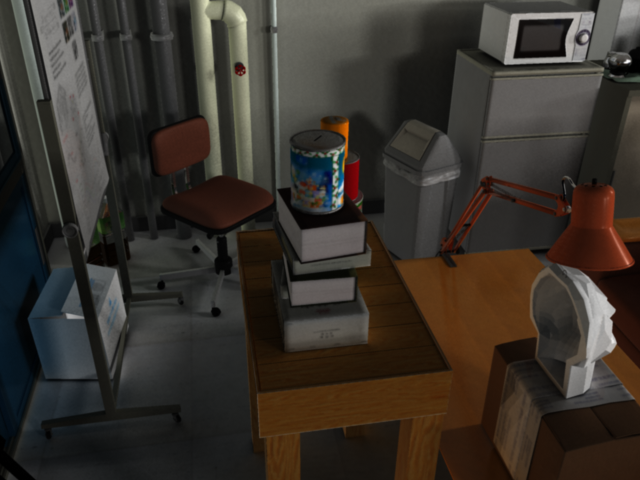
\includegraphics[width=0.40\textwidth]{./images/tsukuba_fluorescent_L_00313.png}
	} 
	\subfloat[Right image]{
		\label{fig:tsukuba_fluorescent_R_00313}
		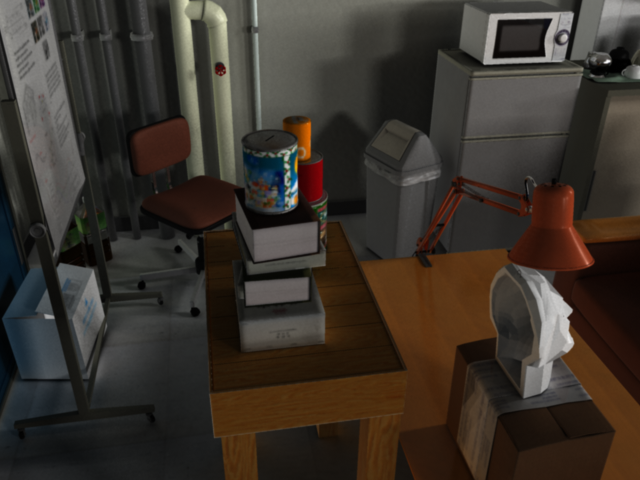
\includegraphics[width=0.40\textwidth]{./images/tsukuba_fluorescent_R_00313.png}
	} 
	\caption{Example image pair of New Tsukuba Stereo Dataset with scattered facets \cite{nakamuraOcclusionDetectableStereoocclusion1996}}
	\label{fig:tsukuba_fluorescent_00313}
\end{figure}
\begin{figure}[htbp]\centering
	\subfloat[Left Image]{
		\label{fig:tsukuba_fluorescent_L_00566}
		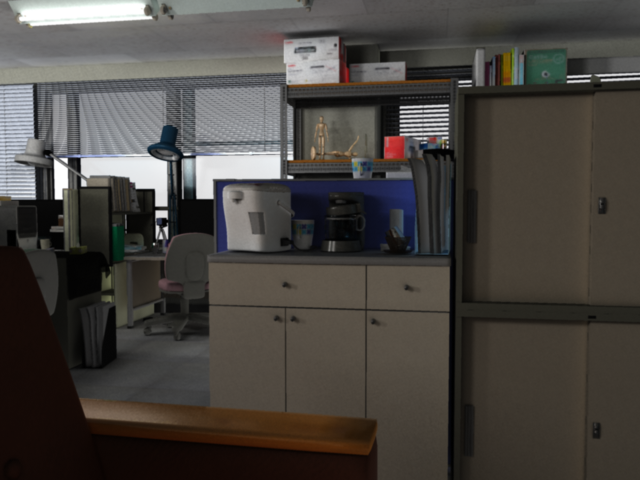
\includegraphics[width=0.40\textwidth]{./images/tsukuba_fluorescent_L_00566.png}
	} 
	\subfloat[Right Image]{
		\label{fig:tsukuba_fluorescent_R_00566}
		\includegraphics[width=0.40\textwidth]{./images/tsukuba_fluorescent_R_00566.png}
	} 
	\caption{Example image pair of New Tsukuba Stereo Dataset with no feature plane \cite{nakamuraOcclusionDetectableStereoocclusion1996}}
	\label{fig:tsukuba_fluorescent_00566}
\end{figure}

AdelaideRMF is a data set for robust geometric model fitting (homography estimation and fundamental matrix estimation). It collects a set of image pairs and the key-point correspondences which were obtained by SIFT matching are manually labeled\cite{wongDynamicHierarchicalMultistructure2011}. Unlike New Tsukuba Stereo Dataset, most of the scenes in it are different buildings, so there are a lot of large flat planes in images \cref{fig:ladysmomo}, such as the wall of red building.
\begin{figure}[htbp]\centering
	\subfloat[Left image]{
		\label{fig:ladysmom1}
		\includegraphics[width=0.50\textwidth]{./images/ladysmom1}
	} \hspace{-2mm}
	\subfloat[Right image]{
		\label{fig:ladysmom2}
		\includegraphics[width=0.50\textwidth]{./images/ladysmom2}
	} 
	\caption{Example image pair of AdelaideRMF Dataset \cite{wongDynamicHierarchicalMultistructure2011}}
	\label{fig:ladysmomo}
\end{figure}

The purpose of evaluation is to evaluate the result of my algorithm, then ground truth is needed for reference. But in AdelaideRMF, there are only matching features that were obtained by SIFT matching. And they can be used to to estimate the homography matrix. But this result is still an approximate value, not a ground truth. So it's meaningless to compare with this result. In other words, this data set can only be used to show the results of our algorithm, but not to verify the accuracy of our algorithm.
\begin{figure}[htbp]\centering
	\subfloat[Barn 1]{
		\label{fig:barn1}
		\includegraphics[width=0.60\textwidth]{./images/Middlebury_Stereo_Datasets/barn1.png}
	} \\
	\subfloat[Barn 2]{
		\label{fig:barn2}
		\includegraphics[width=0.60\textwidth]{./images/Middlebury_Stereo_Datasets/barn2.png}
	} \\
	\subfloat[Bull]{
		\label{fig:bull}
		\includegraphics[width=0.60\textwidth]{./images/Middlebury_Stereo_Datasets/bull.png}
	}\\		
	\caption{Middlebury Stereo Vision Datasets 2001 Version(1) \cite{scharsteinTaxonomyEvaluationDense2001}}
	\label{fig: Middlebury Stereo Vision Datasets 2001 Version(1)}
\end{figure}

\begin{figure}
	
	\centering
	\subfloat[Poster]{
		\label{fig:poster}
		\includegraphics[width=0.60\textwidth]{./images/Middlebury_Stereo_Datasets/poster.png}
	} \\
	\subfloat[Swatooth]{
		\label{fig:swatooth}
		\includegraphics[width=0.60\textwidth]{./images/Middlebury_Stereo_Datasets/swatooth.png}
	} \\
	\subfloat[Venus]{
		\label{fig:venus}
		\includegraphics[width=0.60\textwidth]{./images/Middlebury_Stereo_Datasets/venus.png}
	} 
	\caption{Middlebury Stereo Vision Datasets 2001 Version(2) \cite{scharsteinTaxonomyEvaluationDense2001}}
	\label{Middlebury Stereo Vision Datasets 2001 Version(2)}
\end{figure}

In the end, I introduce Middlebury Stereo Vision Datasets. I mainly used the 2001 Stereo datasets in it with ground truth. There are 6 datasets of piecewise planar scenes \cref{fig: Middlebury Stereo Vision Datasets 2001 Version(1)} and \cref{Middlebury Stereo Vision Datasets 2001 Version(2)}. Because the image pairs in this dataset is all perfect rectified, they can only be use to evaluate the rectified case. 

Besides these stereo image datasets, there are also some available aerial image datasets. But the most datasets don't contain stereo images. Only a small part of them have stereo images, such as ASL Datasets  \url{http://projects.asl.ethz.ch/datasets/} and CMLA Subpixel Stereo Dataset  \url{http://www.ipol.im/pub/pre/187/}. But they either don't have flat plane structure, or they don't have a ground truth. So I don't consider them further.

Because the public datasets, that I could find, are only partly suited for the evaluation of the proposed algorithm. I decided to build my own dataset to verify the algorithm.
\section{Self-Built Datasets} \label{sec:Self-Built Datasets}
In order to construct our own dataset, I first need a virtual environment. I choose Blender as the software for the build environment. Blender is used to manage the 3D scene and do the rendering. There can be some exact objects built by Blender in the virtual environment. In our case, we only need the plane patches in the images. So I just put some planes, which are shading with some pictures, in the scene and render the realistic images. The whole dataset is available online at: \url{https://github.com/Zauberr/Multi-H-Dataset}

The interface of the software is shown in \cref{fig:Interface of Blender}
\begin{figure}[htbp]
	\centering
	\includegraphics[width=0.80\textwidth]{images/Blender/software_interface.png}
	\caption{Interface of Blender}
	\label{fig:Interface of Blender}
\end{figure}

We can see from it that the central main interface is a constructed virtual scene, in which the world coordinate system is preset, red is the x-axis, green is the y-axis and blue is the z-axis. Each object (rigid body) has its own position coordinates and rotation parameters relative to the world coordinate system. In the toolbar at bottom right corner of the screen, we can set the specific parameters of each object in detail. For example, for the camera we use, we can choose different camera models and different focal lengths, etc.

After understanding the main software situation, we focus on the processing pipeline of dataset. We will use the scene in \cref{fig:Interface of Blender} as an example to explain the entire process in detail. First of all, because the algorithm applies to plane structures, we first put three plane structures in the scene and draw different patterns on the surface of each picture. We  call the plane showing the fox the "fox plane", showing Eiffel Tower "eiffel plane" and the last one "greece plane". (In the whole datasets, the used images are from \url{https://pixabay.com}.) The transformations of these three planes are shown in the \cref{fig:Transformation of example planes}.
\begin{figure}[tbp]
	\centering
	\subfloat[Fox]{
		\label{fig:fox}
		\includegraphics[width=0.20\textwidth]{./images/Blender/brickwall}
	} \quad
	\subfloat[Eiffel Tower]{
		\label{fig:Eiffel Tower}
		\includegraphics[width=0.20\textwidth]{./images/Blender/voronoi_plane}
	} \quad
	\subfloat[Greece]{
		\label{fig:Greece}
		\includegraphics[width=0.20\textwidth]{./images/Blender/markov_plane}
	}
	\caption{Transformation of example planes}
	\label{fig:Transformation of example planes}
\end{figure}

After successfully building the scene with the images, we need to extract the image data (render the image) from the virtual scene. In this step we use the camera components in the software. We placed a pair of stereo camera equipment consisting of two cameras with identical internal parameters (shown in \cref{fig:Inter-parameter of Stereo Cameras}) in front of three planes. 
\begin{figure}[htbp]
	\centering
	\subfloat[]{
		\label{fig:inter_parameter1}
		\includegraphics[width=0.40\textwidth]{./images/Blender/camera_inter_parameter}
	} \quad
	\subfloat[]{
		\label{fig:inter_parameter2}
		\includegraphics[width=0.40\textwidth]{./images/Blender/camera_inter_parameter2}
	} 
	\caption{Internal parameter of stereo cameras}
	\label{fig:Inter-parameter of Stereo Cameras}
\end{figure}

The calculation of imaging process also requires external parameters of the camera, such as rotation and translation. These parameters can also be obtained in the software. The parameters in the example are shown in \cref{fig:External-parameter of Stereo Cameras}
\begin{figure}[htbp]
	\centering
	\subfloat[Left Camera]{
		\label{fig:external_parameter1}
		\includegraphics[width=0.30\textwidth]{./images/Blender/camera_external_parameter}
	} \quad
	\subfloat[Right Camera]{
		\label{fig:external_parameter2}
		\includegraphics[width=0.30\textwidth]{./images/Blender/camera_external_parameter2}
	} 
	\caption{External-parameter of stereo cameras}
	\label{fig:External-parameter of Stereo Cameras}
\end{figure}

After providing the light source in the scene, we have completed the construction of a simple virtual environment. After that, the scene should be rendered and collect the raw image data, which can be automatic done by the software. Next, we need to get the specific imaging formula corresponding to our image and the homography matrix of the plane in it, which is regarded as ground truth.

The specific imaging process and formula are exactly the same as described in \cref{sec:main idea}. Finally, we use the \cref{eq:Multiplehomographymatri} to solve homography matrix for each plane. And here I add how to get the parameter matrices needed in \cref{eq:Multiplehomographymatri} based on the actual virtual environment parameters.

For convenience, \cref{eq:Multiplehomographymatri} is repeated here:
\begin{align}
	H=K_{2}R_{2}^T R_{1}K_{1}^{-1}+K_{2}R_{2}^T(\rdc_{1}-\rdc_{2})\cdot \frac{\vec{n}_n^{T}}{d_n}R_{1}K_{1}^{-1}\nonumber
\end{align}
where 
\begin{itemize}
	\item $\rdc_{1},\rdc_{2}$ : location of the camera center in the world coordinate system
	\item $R_{1},R_{2}$: rotation matrix of world coordinate system relative to the camera
	\item $K_{1},K_{2}$: calibration matrix of camera
	\item $\vec{n}_n$: unit outward normal vector of plane
	\item $d_n$: distance from the plane to camera center $C_1$
\end{itemize}

I use the virtual scene shown previously as an example to solve each parameter separately in the equation. In the process of solving each parameter, the meaning of parameters in the formula is the same as the  meaning in each source picture. And the left camera is camera 1.
\begin{itemize}
	\item {\Large $\rdc_{1},\rdc_{2}$}: \\
	From \cref{fig:External-parameter of Stereo Cameras}, we can get the transform information for stereo camera pairs. we can use the location information shown to describe $\rdc_{1},\rdc_{2}$:
	\begin{align}
		\rdc = \begin{bmatrix}
		X\\
		Y\\
		Z
		\end{bmatrix}= \begin{bmatrix}8 \\-7\\5 \end{bmatrix}
	\end{align}
	\item {\Large $R_{1},R_{2}$}: \\
	From \cref{fig:External-parameter of Stereo Cameras}, we can get the transform information for stereo camera pairs. we can use the Rotation information shown to describe $R_{1},R_{2}$ \cite{bernerTechnicalConceptsOrientation2008}, and in blender, it uses extrinsic parameters, in other words, space-fixed rotation.
	\begin{align}
		R &= R_z(Z) R_y(Y) R_x(X) \nonumber \\
			& = R_z(50^{\circ}) R_y(0^{\circ}) R_x(65^{\circ}) \nonumber \\
			& = \begin{bmatrix}
			\cos Z \cos Y & \cos Z \sin Y \sin X - \sin Z \cos X& \cos Z \sin Y \cos X + \sin Z \sin X\\
			\sin Z \cos Y & \sin Z \sin Y \sin X + \cos Z \cos X & \sin Z \sin Y \cos X -\cos Z \sin X \\
			-\sin Y& \cos Y \sin X& \cos Y \cos X
		\end{bmatrix}
	\end{align}

	\item {\Large $K_{1},K_{2}$}: \\
	From \cref{fig:Inter-parameter of Stereo Cameras}, we can get the focal length of camera $f$, sensor width $x$, sensor height $y$ and resolution $X$ and $Y$. The output pixel in the image is set as squared pixel. The scaling factors $k_{x}, k_{y}$ are
	\begin{align}
		k_{x} = k_{y} = \frac{\sqrt{X^2 + Y^2}}{\sqrt{x^2 + y^2}} = \frac{\sqrt{1200^2 + 800^2}}{\sqrt{12^2 + 8^2}} = 100 px/mm 
	\end{align}
	then $K_{1},K_{2}$:
	\begin{align}
	K = K_{1}=K_{2} = \begin{bmatrix}
	f k_{x} & 0 & \frac{X-1} {2} & 0 \\
	0 & -f k_{y} &  \frac{Y-1} {2} & 0 \\
	0 & 0 & -1 & 0
	\end{bmatrix} 
	\end{align}
	where the minus for $f k_{y}$ and $1$ comes from converting coordinate between right-up-backwards coordinate system of Blender and right-down-forward coordinate system of OpenCV.
	
	\item {\Large $\vec{n}_n$}: \\
	From \cref{fig:Transformation of example planes}, we can get location and rotation of each plane. And the unit outward normal vector of each plane before transformation is set by software $\vec{n}_{init} = (0, 0, 1)^T$. So $\vec{n}_n$:
	\begin{align}
		\vec{n} &= R_{plane} \cdot \vec{n}_{init} \nonumber \\
						&= \begin{bmatrix}
							\cos Z \cos Y & \cos Z \sin Y \sin X - \sin Z \cos X& \cos Z \sin Y \cos X + \sin Z \sin X\\
							\sin Z \cos Y & \sin Z \sin Y \sin X + \cos Z \cos X & \sin Z \sin Y \cos X -\cos Z \sin X \\
							-\sin Y& \cos Y \sin X& \cos Y \cos X
						\end{bmatrix} \begin{bmatrix}
						0\\0\\1
						\end{bmatrix}
	\end{align}
	\item {\Large $d_n$}: \\
	Here we regard the right camera as the camera 1. From \cref{fig:external_parameter2}, we know the location of the camera 1 $\rdc_1$ and from \cref{fig:Transformation of example planes}, we can get a point $\vec{t} = (1, -1, 1)^T$ on the plane, which is the same as location of plane. So $d_n$:
	\begin{align}
	d_n = \vec{n}_n^T \rdc_1 - \vec{n}_n^T \vec{t}
	\end{align}
\end{itemize}

Combine all the equation above, we can finally calculate the ground truth: 
\begin{itemize}
	\item $H_{\infty}=K_{2}R_{2}R_{1}^{T}K_{1}^{-1}$
	\item $\vec{e}=K_{2}R_{2}(\rdc_{1}-\rdc_{2})$
	\item $\vec{q}_{n}^T=\frac{\vec{n}_n^{T}}{d_n}R_{1}^{-1}K_{1}^{-1}$
	\item $ H_{n} = H_{\infty} + \vec{e} \cdot \vec{q}_{n}^T$
\end{itemize}

\section{Testing}
After completing the collection and pre-processing of the public datasets and the construction of the test dataset, we could use these images to test my algorithm. In this section, some testing results of the algorithm is shown.
\subsection{Testing with Middlebury Stereo Vision Datasets}\label{subsec:Testing with Middlebury Stereo Vision Datasets}
First, we apply my algorithm on the dataset of Middlebury Stereo Vision Datasets 2001 Version. Just like mention before, the images in the dataset are all rectified. So we use it only to test the rectified case of the algorithm. The results of all image pairs are shown in \cref{fig:Template and transformed plane patches in Middlebury Stereo Vision Datasets} and the PSNR are shown in \cref{tab:PSNR of different patches in  Middlebury Stereo Vision Datasets}. The root mean squared displacement (RMSD) of all patches are shown in \cref{tab:Displacement of different patches for self-built images (1)}.

It can be seen from the results that when the algorithm is applied to the rectified stereo images very stable. That is to say, when $H_{\infty}$ and $\rde$ are known, the result is usually quite accurate. 

\begin{figure}[htbp]\centering
	\subfloat[]{
		\label{fig:Template and transformed plane patches in Middlebury Stereo Vision Datasets (1)}
		\includegraphics[width=0.40\textwidth]{images/Middlebury_Stereo_Datasets/shown1}
	} 
	\subfloat[]{
			\label{fig:Template and transformed plane patches in Middlebury Stereo Vision Datasets (2)}
		\includegraphics[width=0.40\textwidth]{images/Middlebury_Stereo_Datasets/shown2}
	} \\
		\subfloat[]{
		\label{fig:Template and transformed plane patches in Middlebury Stereo Vision Datasets (3)}
		\includegraphics[width=0.40\textwidth]{images/Middlebury_Stereo_Datasets/shown3}
	} 
	\caption{Template and transformed plane patches in Middlebury Stereo Vision Datasets}
	\label{fig:Template and transformed plane patches in Middlebury Stereo Vision Datasets}
\end{figure}

\begin{table}[htbp]
	\centering
	\scriptsize  
	\begin{tabular}{ccccccc} 
		\hline 
		\multicolumn{1}{c}{\multirow{2}{1.2cm}{Shown Figure}} 
		&\multicolumn{5}{c}{Display Patch}  \\ 
		\cline{2-7} 
		&\multicolumn{1}{c}{(1)} & {(2)} & {(3)} & {(4)} & {(5)} & {(6)} \\ 
		\hline 
		\cref{fig:Template and transformed plane patches in Middlebury Stereo Vision Datasets (1)} &37.5768&40.4451&45.9941&42.4099&47.7764&38.3245 \\ 
		\cref{fig:Template and transformed plane patches in Middlebury Stereo Vision Datasets (2)}&46.9869&41.8912&32.6315&41.8892&36.9338&49.0576\\ 
		 \cref{fig:Template and transformed plane patches in Middlebury Stereo Vision Datasets (3)}&51.4393&44.9664&34.969591&47.4049&45.2209&\\ 
		\hline 
	\end{tabular} 
	\caption{PSNR (dB) of different patches in  Middlebury Stereo Vision Datasets}  
	\label{tab:PSNR of different patches in  Middlebury Stereo Vision Datasets} 
\end{table}

\begin{table}[htbp]
	\centering
	\scriptsize  
	\begin{tabular}{ccccccc} 
		\hline 
		\multicolumn{1}{c}{\multirow{2}{1.2cm}{Shown Figure}} 
		&\multicolumn{5}{c}{Display Patch}  \\ 
		\cline{2-7} 
		&\multicolumn{1}{c}{(1)} & {(2)} & {(3)} & {(4)} & {(5)} & {(6)} \\ 
		\hline 
		\cref{fig:Template and transformed plane patches in Middlebury Stereo Vision Datasets (1)} &2.252596&0.647761&0.184386&0.536102&0.954197&0.895281\\ 
		\cref{fig:Template and transformed plane patches in Middlebury Stereo Vision Datasets (2)}&0.203423&1.123935&1.523684&0.358562&1.111534&0.102031\\ 
		\cref{fig:Template and transformed plane patches in Middlebury Stereo Vision Datasets (3)}&0.507921&0.344584&1.353465&0.664646&0.188721&\\ 
		\hline 
	\end{tabular} 
	\caption{Displacement (pixel) of different patches in  Middlebury Stereo Vision Datasets}  
	\label{tab:Displacement of different patches in  Middlebury Stereo Vision Datasets} 
\end{table}

\subsection{Testing with Self-built Stereo Images}\label{subsec:Testing with Self-built Stereo Images}
When the algorithm is applied to the image pair without ground truth, the evaluation could only be done with the difference image and PSNR. Next, we will focus on application on the self-built testing images with ground truth. The evaluation can be done with the ground truth.

I start also with the rectified stereo images. The built images is shown in \cref{fig:Self-built Stereo Images}. And the ground truth of it was calculated in the way mentioned in \cref{sec:Self-Built Datasets}. Using algorithm on the images, the result is shown in \cref{fig:Result of Self-built Stereo Images} and the estimated parameters are in \cref{tab:Ground Truth and Estimated Parameter for self-built Stereo Images}. PSNR is in \cref{tab:PSNR of different patches for Self-built Stereo Images}. The root mean squared displacement (RMSD) and maximum displacement of all patches are shown in \cref{tab:Displacement of different patches for self-built stereo images}.

\begin{figure}[tbp]\centering
	\subfloat[Template image]{
		\label{fig:Template Image11}
		\includegraphics[width=0.30\textwidth]{images/Evaluation/Stereo_case/patch_1_ROI_of_template}
	}  \hspace{-2mm}
	\subfloat[Warped image for mercury plane]{
		\label{fig:Warped Image For Mercury Plane}
		\includegraphics[width=0.30\textwidth]{images/Evaluation/Stereo_case/patch_1_ROI_of_warped_image}
	} \hspace{-2mm}
	\subfloat[Difference image]{
		\label{fig:Difference Image11}
		\includegraphics[width=0.30\textwidth]{images/Evaluation/Stereo_case/patch_1_difference}
	}\hspace{-2.5mm}
	\subfloat[]{
	%		\label{fig:diffBill}
	\includegraphics[height = 3.9cm]{./images/legendH}
} 
\\
	
		\subfloat[Template image]{
		\label{fig:Template Image21}
		\includegraphics[width=0.30\textwidth]{images/Evaluation/Stereo_case/patch_2_ROI_of_template}
	}  \hspace{-2mm}
	\subfloat[Warped image for sheep plane]{
		\label{fig:Warped Image For Sheep Plane}
		\includegraphics[width=0.30\textwidth]{images/Evaluation/Stereo_case/patch_2_ROI_of_warped_image}
	} \hspace{-2mm}
	\subfloat[Difference image]{
		\label{fig:Difference Image21}
		\includegraphics[width=0.30\textwidth]{images/Evaluation/Stereo_case/patch_2_difference}
	}\hspace{-2.5mm}
	\subfloat[]{
	%		\label{fig:diffBill}
	\includegraphics[height = 4.3cm]{./images/legendH}
} 
\\

		\subfloat[Template image]{
		\label{fig:Template Image211}
		\includegraphics[width=0.30\textwidth]{images/Evaluation/Stereo_case/patch_3_ROI_of_template}
	}  \hspace{-2mm}
	\subfloat[Warped image for butterfly plane]{
		\label{fig:Warped Image For Butterfly Plane}
		\includegraphics[width=0.30\textwidth]{images/Evaluation/Stereo_case/patch_3_ROI_of_warped_image}
	} \hspace{-2mm}
	\subfloat[Difference image]{
		\label{fig:Difference Image31}
		\includegraphics[width=0.30\textwidth]{images/Evaluation/Stereo_case/patch_3_difference}
	}\hspace{-2.5mm}
	\subfloat[]{
	%		\label{fig:diffBill}
	\includegraphics[height = 2.2cm]{./images/legendH}
} 

	\caption{Result of self-built stereo images}
	\label{fig:Result of Self-built Stereo Images}
\end{figure}

\begin{table}[tbp]
	\centering
	\scriptsize  
	\begin{tabular}{p{80pt} p{60pt}}
		\toprule
		Patch & {\bfseries PSNR(dB)}\\ \midrule
		Mercury Plane&  49.1514\\
		\addlinespace[3pt]
		Sheep Plane  &  66.9878\\
		\addlinespace[3pt]
		Butterfly Plane & 56.9686 \\ \bottomrule
	\end{tabular}
	\caption{PSNR of different patches for self-built stereo images}  
	\label{tab:PSNR of different patches for Self-built Stereo Images} 
\end{table}

\begin{table}[htbp]
	\centering
	\scriptsize  
	\begin{tabular}{p{80pt} p{60pt} p{60pt}}
		\toprule
		Patch & {\bfseries RMSD (pixel)} & {\bfseries Maximum(pixel)}\\ \midrule
		Mercury Plane&  0.044846&0.045849 \\
		\addlinespace[3pt]
		Sheep Plane  &  0.003704&0.004460 \\
		\addlinespace[3pt]
		Butterfly Plane & 0.017901&0.018868\\ \bottomrule
	\end{tabular}
	\caption{Displacement of different patches for self-built stereo images}  
	\label{tab:Displacement of different patches for self-built stereo images} 
\end{table}

\begin{table}[htbp]
	\centering
	\scriptsize  
	\begin{tabular}{ccc}
		\toprule
		\bfseries Parameter & \bfseries Ground Truth &\bfseries Estimated \\ \midrule
		$H_\infty$   &  $\begin{bmatrix}1 &0&0 \\
		0&1& 0\\
		0& 0&1\\ \end{bmatrix}$ &$\begin{bmatrix}1 &0&0 \\
		0&1& 0\\
		0& 0&1\\ \end{bmatrix}$  \\
		\addlinespace[5pt]
		$\rde$ & $\begin{bmatrix} -5.69822333e+02 \\
		-4.57549368e-03\\
		1.52790722e-05 \end{bmatrix}$&$\begin{bmatrix} -5.69822333e+02 \\
		-4.57549368e-03\\
		1.52790722e-05 \end{bmatrix}$ \\
		\addlinespace[5pt]
		$\vec{q}_1$ & $\begin{bmatrix} -5.04147145e-05 \\
		-2.53917154e-05\\
		1.22084579e-01 \end{bmatrix}$ & $\begin{bmatrix} -5.04285679e-05 \\
		-2.54000998e-05\\
		1.22014162e-01 \end{bmatrix} $ \\
		\addlinespace[5pt]
		$\vec{q}_2$ & $\begin{bmatrix} 6.80928394e-05\\
		-2.41470029e-05 \\
		4.64782197e-02 \end{bmatrix} $ & $\begin{bmatrix} 6.80857568e-05\\
		-2.41376373e-05 \\
		4.64747905e-02 \end{bmatrix}$ \\
		\addlinespace[5pt]
		$\vec{q}_3$ & $ \begin{bmatrix} 0.00000000e+00\\
		1.09855489e-04 \\
		3.28974882e-02 \end{bmatrix}$ & $\begin{bmatrix} -1.58691562e-09\\
		1.09810544e-04 \\
		3.28889686e-02 \end{bmatrix}$ \\
		${r_1}_1$ & &9.96429311e-01\\
		\addlinespace[5pt]
		${r_2}_1$& &  -2.65463250e-05\\
		\addlinespace[5pt]
		${r_1}_2$ & &9.94738600e-01\\
		\addlinespace[5pt]
		${r_2}_2$& & -4.20122298e-05\\
		\addlinespace[5pt]
		${r_1}_3$ & &9.97044402e-01\\
		\addlinespace[5pt]
		${r_2}_3$& & -2.07652871e-05\\
		\addlinespace[5pt]
		\bottomrule
	\end{tabular}
	\caption{Ground truth and estimated parameter for self-built stereo images}  
	\label{tab:Ground Truth and Estimated Parameter for self-built Stereo Images} 
\end{table}

\begin{figure}[tbp]
	\centering
	\subfloat[Template image]{
		\label{fig:temp1}
		\includegraphics[width=0.40\textwidth]{./images/Evaluation/Stereo_case/original_template_img}
	} \quad
	\subfloat[Target image]{
		\label{fig:targ1}
		\includegraphics[width=0.40\textwidth]{./images/Evaluation/Stereo_case/original_target_img}
	} 
	\caption{Self-built stereo images}
	\label{fig:Self-built Stereo Images}
\end{figure}

\subsection{Testing with Self-built Normal Images}\label{subsec:Testing with Self-built Normal Images}
In this part, the results of testing with the self-built normal images are shown. I have chosen 3 image pairs to evaluate the algorithm.

First, a scenario with very different camera poses. The self-built images are shown in \cref{fig:Self-built Images(1)}. The ground truth and estimated parameters are in \cref{tab:Ground Truth and Estimated Parameter(1)}. PSNR is in \cref{tab:PSNR of different patches for Self-built Images(1)}. The root mean squared displacement (RMSD) and maximum displacement of all patches are shown in \cref{tab:Displacement of different patches for self-built images (1)}. The warped images are shown in \cref{fig:Result of Self-built Normal Images(1)}. From this result, we know that the result of brick-wall plane is not very good. The reason is that the algorithm sometimes responds to the texture structure not very well. In order to overcome it, we should use the image pyramid. 

What's more, the camera poses are very different and the algorithm can also find the correct result with suitable initialization. This proves that the algorithm can be applied on any two pictures, as long as they contain the same planes.
\begin{figure}[htbp]
	\centering
	\subfloat[Template image]{
		\label{fig:temp111}
		\includegraphics[width=0.40\textwidth]{./images/Evaluation/Normal_case1/original_template_img}
	} \quad
	\subfloat[Target image]{
		\label{fig:targ111}
		\includegraphics[width=0.40\textwidth]{./images/Evaluation/Normal_case1/original_target_img}
	} 
	\caption{Self-built images (1)}
	\label{fig:Self-built Images(1)}
\end{figure}

\begin{figure}[htbp]\centering
	\subfloat[Template image]{
		\label{fig:Template Image111}
		\includegraphics[width=0.30\textwidth]{images/Evaluation/Normal_case1/patch_1_ROI_of_template}
	} \hspace{-2mm} 
	\subfloat[Warped image for brick-wall plane]{
		\label{fig:Warped Image For Brick-wall Plane}
		\includegraphics[width=0.30\textwidth]{images/Evaluation/Normal_case1/patch_1_ROI_of_warped_image}
	} \hspace{-2mm}
	\subfloat[Difference image]{
		\label{fig:Difference Image111}
		\includegraphics[width=0.30\textwidth]{images/Evaluation/Normal_case1/patch_1_difference}
	}\hspace{-2.5mm}
	\subfloat[]{
	%		\label{fig:diffBill}
	\includegraphics[height = 3.5cm]{./images/legendH}
} 
\\
	\subfloat[Template image]{
		\label{fig:Template Image2111}
		\includegraphics[width=0.29\textwidth]{images/Evaluation/Normal_case1/patch_2_ROI_of_template}
	}  \hspace{-2mm}
	\subfloat[Warped image for voronoi plane]{
		\label{fig:Warped Image For Voronoi Plane}
		\includegraphics[width=0.29\textwidth]{images/Evaluation/Normal_case1/patch_2_ROI_of_warped_image}
	} \hspace{-2mm}
	\subfloat[Difference image]{
		\label{fig:Difference Image211}
		\includegraphics[width=0.29\textwidth]{images/Evaluation/Normal_case1/patch_2_difference}
	}\hspace{-2.5mm}
	\subfloat[]{
	%		\label{fig:diffBill}
	\includegraphics[height = 5.2cm]{./images/legendH}
} 
\\
	
	\subfloat[Template image]{
		\label{fig:Template Image21111}
		\includegraphics[width=0.30\textwidth]{images/Evaluation/Normal_case1/patch_3_ROI_of_template}
	}  \hspace{-2mm}
	\subfloat[Warped image for markov plane]{
	
		\includegraphics[width=0.30\textwidth]{images/Evaluation/Normal_case1/patch_3_ROI_of_warped_image}
	} \hspace{-2mm}
	\subfloat[Difference image]{
		\label{fig:Difference Image311}
		\includegraphics[width=0.30\textwidth]{images/Evaluation/Normal_case1/patch_3_difference}
	}\hspace{-2.5mm}
	\subfloat[]{
	%		\label{fig:diffBill}
	\includegraphics[height = 2.3cm]{./images/legendH}
} 
\\
	\caption{Result of self-built normal images (1)}
	\label{fig:Result of Self-built Normal Images(1)}
\end{figure}

\begin{table}[tbp]
	\centering
	\scriptsize  
	\begin{tabular}{p{80pt} p{60pt}}
		\toprule
		Patch & {\bfseries PSNR(dB)}\\ \midrule
		Brick-wall Plane&  29.3573\\
		\addlinespace[3pt]
		Voronoi Plane  &  40.4581\\
		\addlinespace[3pt]
		Markov Plane &38.8231 \\ \bottomrule
	\end{tabular}
	\caption{PSNR of different patches for self-built images (1)}  
	\label{tab:PSNR of different patches for Self-built Images(1)} 
\end{table}

\begin{table}[htbp]
	\centering
	\scriptsize 
	\begin{tabular}{p{80pt} p{60pt} p{60pt}}
		\toprule
		Patch & {\bfseries RMSD (pixel)} & {\bfseries Maximum(pixel)}\\ \midrule
		Brick-wall Plane&  0.304703&0.325780 \\
		\addlinespace[3pt]
		Voronoi Plane  &  0.208013&0.277421 \\
		\addlinespace[3pt]
		Markov Plane & 0.344370&0.397986 \\ 
		\addlinespace[3pt]
		All Patches & 0.288475&0.397986 \\ \bottomrule
	\end{tabular}
	\caption{Displacement of different patches for self-built images (1)}  
	\label{tab:Displacement of different patches for self-built images (1)} 
\end{table}

\begin{table}[htbp]
	\centering
	\tiny 
	\begin{tabular}{ccc}
		\toprule
		\bfseries Parameter & \bfseries Ground Truth &\bfseries Estimated \\ \midrule
		$H_\infty$   &  $\begin{bmatrix}9.65703446e-01 &-8.36839711e-03&1.39138794e+02 \\
		2.19264412e-02&1.01576119e+00& -1.23767980e+02\\
		-5.08187535e-05& 4.74420190e-05&1.00606213e+00 \end{bmatrix}$ &$\begin{bmatrix}9.65839836e-01 &-8.41589335e-03 & 1.39060980e+02 \\
		2.19485280e-02 & 1.01520898e+00& -1.23718912e+02\\
		-5.05974374e-05  &4.74229252e-05 & 1.00579468e+00 \end{bmatrix}$  \\
		\addlinespace[5pt]
		$\rde$ & $\begin{bmatrix} -7.24246259e+02 \\
		-1.64515557e+01\\
		3.81296513e-02 \end{bmatrix}$&$\begin{bmatrix} -7.24204197e+02 \\
		-1.64534715e+01\\
		4.01498913e-02 \end{bmatrix}$ \\
		\addlinespace[5pt]
		$\vec{q}_1$ & $\begin{bmatrix} -5.96261061e-05 \\
		-3.00310957e-05\\
		1.44390941e-01 \end{bmatrix}$ & $\begin{bmatrix} -5.96507588e-05 \\
		-3.02164145e-05\\
		1.44743346e-01 \end{bmatrix}$ \\
		\addlinespace[5pt]
		$\vec{q}_2$ & $\begin{bmatrix}8.15476596e-05 \\-2.89183354e-05 \\ 5.56620941e-02\end{bmatrix}$ & $\begin{bmatrix}  8.14932969e-05\\
		-2.88990747e-05\\
		5.57176245e-02 \end{bmatrix}$ \\
		\addlinespace[5pt]
		$\vec{q}_3$ & $\begin{bmatrix} 0.00000000e+00  \\1.15523713e-04 \\ 3.45949029e-02 \end{bmatrix}$ & $\begin{bmatrix}1.89395051e-07\\
		1.14948256e-04\\
		3.49029342e-02 \end{bmatrix}$ \\
		${r_1}_1$ & &9.93390769e-01\\
		\addlinespace[5pt]
		${r_2}_1$& & -4.61817515e-05\\
		\addlinespace[5pt]
		${r_1}_2$ & &9.97370299e-01\\
		\addlinespace[5pt]
		${r_2}_2$& & -1.80821342e-05\\
		\addlinespace[5pt]
		${r_1}_2$ & &9.96350068e-01\\
		\addlinespace[5pt]
		${r_2}_2$& & -3.17773268e-05\\
		\addlinespace[5pt]
		\bottomrule
	\end{tabular}
	\caption{Ground truth and estimated parameter (1)}  
	\label{tab:Ground Truth and Estimated Parameter(1)} 
\end{table}

The second example images pair comes from two cameras with very different poses, too. The self-built images are shown in \cref{fig:Self-built Images(2)}. The ground truth and estimated parameters are in \cref{tab:Ground Truth and Estimated Parameter(2)}. PSNR is in \cref{tab:PSNR of different patches for Self-built Images(2)}.  The root mean squared displacement (RMSD) and maximum displacement of all patches are shown in \cref{tab:Displacement of different patches for self-built images (2)}. The warped images are shown in \cref{fig:Result of Self-built Normal Images(2)}.  There are no texture structure in these images. So the result is all perfect.

\begin{figure}[htbp]
	\centering
	\subfloat[Template image]{
		\label{fig:temp1sdf11}
		\includegraphics[width=0.40\textwidth]{./images/Evaluation/Normal_case3/original_template_img}
	} \quad
	\subfloat[Target image]{
		\label{fig:targ11dwe1}
		\includegraphics[width=0.40\textwidth]{./images/Evaluation/Normal_case3/original_target_img}
	} 
	\caption{Self-built images (2)}
	\label{fig:Self-built Images(2)}
\end{figure}

\begin{figure}[htbp]\centering
	\subfloat[Template image]{
		\label{fig:Template Image1daf11}
		\includegraphics[width=0.30\textwidth]{images/Evaluation/Normal_case3/patch_1_ROI_of_template}
	}\hspace{-2mm}
	\subfloat[Warped image for fantasy plane]{
	
		\includegraphics[width=0.30\textwidth]{images/Evaluation/Normal_case3/patch_1_ROI_of_warped_image}
	}\hspace{-2mm}
	\subfloat[Difference image]{
		\label{fig:Difference Image1we11}
		\includegraphics[width=0.30\textwidth]{images/Evaluation/Normal_case3/patch_1_difference}
	}\hspace{-2.5mm}
	\subfloat[]{
	%		\label{fig:diffBill}
	\includegraphics[height = 3.2cm]{./images/legendH}
} \\
	
	\subfloat[Template image]{
		\label{fig:Template Image2we111}
		\includegraphics[width=0.30\textwidth]{images/Evaluation/Normal_case3/patch_2_ROI_of_template}
	}\hspace{-2mm}
	\subfloat[Warped image for squirrel plane]{
		\label{fig:Warped Image For Vordsfaonoi Plane}
		\includegraphics[width=0.30\textwidth]{images/Evaluation/Normal_case3/patch_2_ROI_of_warped_image}
	}\hspace{-2mm}
	\subfloat[Difference image]{
		\label{fig:Difference Image2we11}
		\includegraphics[width=0.30\textwidth]{images/Evaluation/Normal_case3/patch_2_difference}
	}\hspace{-2.5mm}
	\subfloat[]{
	%		\label{fig:diffBill}
	\includegraphics[height = 4.7cm]{./images/legendH}
} \\
	\subfloat[Template image]{
		\label{fig:Template Image21we111}
		\includegraphics[width=0.30\textwidth]{images/Evaluation/Normal_case3/patch_3_ROI_of_template}
	}\hspace{-2mm}  
	\subfloat[Warped image for sparrow plane]{
		\label{fig:Warped Image For Marwekov Planweqwee}
		\includegraphics[width=0.30\textwidth]{images/Evaluation/Normal_case3/patch_3_ROI_of_warped_image}
	}\hspace{-2mm}
	\subfloat[Difference image]{
		\label{fig:Difference Image3we11}
		\includegraphics[width=0.30\textwidth]{images/Evaluation/Normal_case3/patch_3_difference}
	}\hspace{-2.5mm}
	\subfloat[]{
	%		\label{fig:diffBill}
	\includegraphics[height = 3.4cm]{./images/legendH}
} 

	\caption{Result of self-built normal images (2)}
	\label{fig:Result of Self-built Normal Images(2)}
\end{figure}

\begin{table}[tbp]
	\centering
	\scriptsize  
	\begin{tabular}{p{80pt} p{60pt}}
		\toprule
		Patch & {\bfseries PSNR(dB)}\\ \midrule
		Fantasy Plane&  36.1911\\
		\addlinespace[3pt]
		Squirrel Plane  &  40.2400\\
		\addlinespace[3pt]
		Sparrow Plane &40.4210\\ \bottomrule
	\end{tabular}
	\caption{PSNR of different patches for self-built images (2)}  
	\label{tab:PSNR of different patches for Self-built Images(2)} 
\end{table}

\begin{table}[htbp]
	\centering
	\scriptsize 
	\begin{tabular}{p{80pt} p{60pt} p{60pt}}
		\toprule
		Patch & {\bfseries RMSD (pixel)} & {\bfseries Maximum(pixel)}\\ \midrule
		Fantasy Plane&  0.291320&0.393618 \\
		\addlinespace[3pt]
		Squirrel Plane  &  0.131122&0.154218 \\
		\addlinespace[3pt]
		Sparrow Plane & 0.189493&0.207162 \\ 
		\addlinespace[3pt]
		All Patches & 0.202340&0.393618 \\ \bottomrule
	\end{tabular}
	\caption{Displacement of different patches for self-built images (2)}  
	\label{tab:Displacement of different patches for self-built images (2)} 
\end{table}

\begin{table}[htbp]
	\centering
	\tiny 
	\begin{tabular}{ccc}
		\toprule
		\bfseries Parameter & \bfseries Ground Truth &\bfseries Estimated \\ \midrule
		$H_\infty$   &  $\begin{bmatrix}9.52824171e-01& -1.61137624e-01&  2.06105992e+02 \\
		1.88784031e-01&  1.00060579e+00 &-2.35871911e+02\\
		-4.01833405e-05 & 6.27021960e-05 & 9.92769988e-01 \end{bmatrix}$ &$\begin{bmatrix}9.51958568e-01& -1.61028691e-01&  2.05291642e+02 \\
		1.88447546e-01&  9.99411077e-01 &-2.35358036e+02\\
		-3.99424923e-05&  6.26078118e-05&  9.90950379e-01 \end{bmatrix}$  \\
		\addlinespace[5pt]
		$\rde$ & $\begin{bmatrix} -1.21556156e+03 \\-4.60188500e+01\\ -7.75948410e-02 \end{bmatrix}$&$\begin{bmatrix} -1.21004890e+03\\
		-4.60502141e+01\\
		-7.27863792e-02 \end{bmatrix}$ \\
		\addlinespace[5pt]
		$\vec{q}_1$ & $\begin{bmatrix} -3.18191743e-05\\ -3.30706122e-06\\  1.00547129e-01 \end{bmatrix}$ & $\begin{bmatrix} -3.20962545e-05\\
		-4.33730691e-06\\
		1.00806139e-01 \end{bmatrix}$ \\
		\addlinespace[5pt]
		$\vec{q}_2$ & $\begin{bmatrix}5.10113553e-05\\ -1.23551078e-05 \\ 5.98174870e-02\end{bmatrix}$ & $\begin{bmatrix}   5.10028797e-05\\
		-1.23051622e-05\\
		5.98152421e-02 \end{bmatrix}$ \\
		\addlinespace[5pt]
		$\vec{q}_3$ & $\begin{bmatrix} 1.06495815e-05  \\4.19802260e-05 \\ 7.33070552e-02 \end{bmatrix}$ & $\begin{bmatrix}1.05603440e-05\\
		4.18628465e-05\\
		7.33696013e-02 \end{bmatrix}$ \\
		${r_1}_1$ & &1.01451717e+00\\
		\addlinespace[5pt]
		${r_2}_1$& & 1.17515309e-04\\
		\addlinespace[5pt]
		${r_1}_2$ & & 9.86832299e-01\\
		\addlinespace[5pt]
		${r_2}_2$& & -1.10771571e-04\\
		\addlinespace[5pt]
		${r_1}_2$ & &9.96963583e-01\\
		\addlinespace[5pt]
		${r_2}_2$& & -1.98783474e-05\\
		\addlinespace[5pt]
		\bottomrule
	\end{tabular}
	\caption{Ground truth and estimated parameter (2)}  
	\label{tab:Ground Truth and Estimated Parameter(2)} 
\end{table}

Finally, I show a result of a pair of unrectified stereo images. The self-built images are shown in \cref{fig:Self-built Images(3)}. The ground truth and estimated parameters are in \cref{tab:Ground Truth and Estimated Parameter(3)}. PSNR is in \cref{tab:PSNR of different patches for Self-built Images(3)}. The root mean squared displacement (RMSD) and maximum displacement of all patches are shown in \cref{tab:Displacement of different patches for self-built images (3)}. The warped images are shown in \cref{fig:Result of Self-built Normal Images(3)}.

\begin{figure}[htbp]
	\centering
	\subfloat[Template image]{
		\label{fig:temp1sdf1we1}
		\includegraphics[width=0.40\textwidth]{./images/Evaluation/Normal_case4/original_template_img}
	} \quad
	\subfloat[Target image]{
		\label{fig:targ11dewe1}
		\includegraphics[width=0.40\textwidth]{./images/Evaluation/Normal_case4/original_target_img}
	} 
	\caption{Self-built images (3)}
	\label{fig:Self-built Images(3)}
\end{figure}

\begin{figure}[htbp]\centering
	\subfloat[Template image]{
		\label{fig:Template Imsdage1daf11}
		\includegraphics[width=0.30\textwidth]{images/Evaluation/Normal_case4/patch_1_ROI_of_template}
	}\hspace{-2mm}
	\subfloat[Warped image for fox plane]{
		\label{fig:Warped Image For Bricwewek-wall Plane}
		\includegraphics[width=0.30\textwidth]{images/Evaluation/Normal_case4/patch_1_ROI_of_warped_image}
	}\hspace{-2mm}
	\subfloat[Difference image]{
		\label{fig:Difference Imawege1we11}
		\includegraphics[width=0.30\textwidth]{images/Evaluation/Normal_case4/patch_1_difference}
	}\hspace{-2.5mm}
	\subfloat[]{
	%		\label{fig:diffBill}
	\includegraphics[height = 3.6cm]{./images/legendH}
} \\
	
	\subfloat[Template image]{
		\label{fig:Template Imagewe2we111}
		\includegraphics[width=0.30\textwidth]{images/Evaluation/Normal_case4/patch_2_ROI_of_template}
	}\hspace{-2mm}
	\subfloat[Warped image for eiffel plane]{
		\label{fig:Warped Image For Vordswefaonoi Plane}
		\includegraphics[width=0.30\textwidth]{images/Evaluation/Normal_case4/patch_2_ROI_of_warped_image}
	}\hspace{-2mm}
	\subfloat[Difference image]{
		\label{fig:Difference Imawege2we11}
		\includegraphics[width=0.30\textwidth]{images/Evaluation/Normal_case4/patch_2_difference}
	}\hspace{-2.5mm}
	\subfloat[]{
	%		\label{fig:diffBill}
	\includegraphics[height = 4.2cm]{./images/legendH}
} \\
	
	\subfloat[Template image]{
		\label{fig:Template Imawege21we111}
		\includegraphics[width=0.30\textwidth]{images/Evaluation/Normal_case4/patch_3_ROI_of_template}
	}\hspace{-2mm}
	\subfloat[Warped image for greece plane]{
		\label{fig:Warped Image For Marwewerqwer23232kov Plane}
		\includegraphics[width=0.30\textwidth]{images/Evaluation/Normal_case4/patch_3_ROI_of_warped_image}
	}\hspace{-2mm}
	\subfloat[Difference image]{
		\label{fig:Difference Imweage3we11}
		\includegraphics[width=0.30\textwidth]{images/Evaluation/Normal_case4/patch_3_difference}
	}\hspace{-2.5mm}
	\subfloat[]{
	%		\label{fig:diffBill}
	\includegraphics[height = 3.3cm]{./images/legendH}
} 
	\caption{Result of self-built normal images (3)}
	\label{fig:Result of Self-built Normal Images(3)}
\end{figure}

\begin{table}[tbp]
	\centering
	\scriptsize  
	\begin{tabular}{p{80pt} p{60pt}}
		\toprule
		Patch & {\bfseries PSNR(dB)}\\ \midrule
		Fox Plane&  46.1314\\
		\addlinespace[3pt]
		Eiffel Plane  &  44.7784\\
		\addlinespace[3pt]
		Greece Plane &32.3565\\ \bottomrule
	\end{tabular}
	\caption{PSNR of different patches for self-built images (3)}  
	\label{tab:PSNR of different patches for Self-built Images(3)} 
\end{table}

\begin{table}[htbp]
	\centering
	\scriptsize  
	\begin{tabular}{p{80pt} p{60pt} p{60pt}}
	\toprule
	Patch & {\bfseries RMSD (pixel)} & {\bfseries Maximum(pixel)}\\ \midrule
	Fox Plane&  0.126497&0.226566 \\
	\addlinespace[3pt]
	Eiffel Plane  &  0.087420&0.162986\\
	\addlinespace[3pt]
	Greece Plane & 0.136024&0.194004 \\ 
	\addlinespace[3pt]
	All Patches & 0.117115&0.226566 \\ \bottomrule
	\end{tabular}
	\caption{Displacement of different patches for self-built images (3)}  
	\label{tab:Displacement of different patches for self-built images (3)} 
\end{table}

\begin{table}[htbp]
	\centering
	\tiny
	\begin{tabular}{ccc}
		\toprule
		\bfseries Parameter & \bfseries Ground Truth &\bfseries Estimated \\ \midrule
		$H_\infty$   &  $\begin{bmatrix}9.67030208e-01& -3.13227134e-02 & 1.42036819e+02 \\
		1.54081860e-02 & 1.00157007e+00 &-1.94949553e+01\\
		-4.93452978e-05&  5.50999444e-06 & 1.02462584e+00 \end{bmatrix}$ &$\begin{bmatrix}9.89508997e-01& -3.14215411e-02  &1.41579233e+02 \\
		1.61180210e-02&  1.02097858e+00& -2.02384459e+01\\
		-4.89309883e-05&  6.50245995e-06&  1.03992663e+00 \end{bmatrix}$  \\
		\addlinespace[5pt]
		$\rde$ & $\begin{bmatrix} -1.19028099e+03 \\-1.55712365e+00\\  4.98674731e-03 \end{bmatrix}$&$\begin{bmatrix} -1.19003604e+03\\
		-1.62088391e+00\\
		3.23745088e-02 \end{bmatrix}$ \\
		\addlinespace[5pt]
		$\vec{q}_1$ & $\begin{bmatrix}-4.45934748e-05\\ -2.22353073e-05\\  1.08137896e-01 \end{bmatrix}$ & $\begin{bmatrix} -4.18794095e-05\\
		2.10081204e-05\\
		1.07554103e-01 \end{bmatrix}$ \\
		\addlinespace[5pt]
		$\vec{q}_2$ & $\begin{bmatrix}4.89262638e-05\\ -1.18500922e-05 \\ 5.73724445e-02\end{bmatrix}$ & $\begin{bmatrix}   5.09498850e-05\\
		-1.22376789e-05\\
		5.80580159e-02 \end{bmatrix}$ \\
		\addlinespace[5pt]
		$\vec{q}_3$ & $\begin{bmatrix}-1.00128972e-05\\  1.09754268e-05\\  9.83050209e-02 \end{bmatrix}$ & $\begin{bmatrix}-7.76330602e-06\\
		1.09390874e-05\\
		9.86232716e-02 \end{bmatrix}$ \\
		${r_1}_1$ & &9.99853298e-01\\
		\addlinespace[5pt]
		${r_2}_1$& & -1.25598370e-06\\
		\addlinespace[5pt]
		${r_1}_2$ & & 9.94348907e-01\\
		\addlinespace[5pt]
		${r_2}_2$& & -3.45616975e-05\\
		\addlinespace[5pt]
		${r_1}_2$ & &1.02688585e+00\\
		\addlinespace[5pt]
		${r_2}_2$& & 1.64952502e-04\\
		\addlinespace[5pt]
		\bottomrule
	\end{tabular}
	\caption{Ground truth and estimated parameter (3)}  
	\label{tab:Ground Truth and Estimated Parameter(3)} 
\end{table}

\clearpage

\subsection{Comparison and analysis}
So far, the proposed algorithm is applied to the self-built images and Middlebury Stereo Vision Datasets. The specific test results obtained are listed in detail in \cref{subsec:Testing with Middlebury Stereo Vision Datasets}, \cref{subsec:Testing with Self-built Stereo Images},  \cref{subsec:Testing with Self-built Normal Images}, \cref{subsec:Rectified Stereo Images} and \cref{subsec:Unrectified Images}. For datasets with ground truth, we can analyze our algorithm by comparing the estimated result with the ground truth.

I summarize all the results of image pairs with ground truth in \cref{tab:Result of rectified stereo testing images} and \cref{tab:Result of unrectified testing images}.

\begin{table}[htbp]
	\centering
	\scriptsize   
	\begin{tabular}{ccccc}
		\toprule
		Image Pair & Patch & {\bfseries RMSD (pixel)} & {\bfseries Maximum(pixel)}&{\bfseries PSNR(dB)}\\ \midrule
		\multirow{6}{80pt}{\centering \cref{fig:Template and transformed plane patches in Middlebury Stereo Vision Datasets (1)}}&(1)&  2.252596&3.125&37.5768\\
		\addlinespace[3pt]
		&(2)  &  0.647761&0.975361&40.4451 \\
		\addlinespace[3pt]
		&(3) & 0.184386&0.324421&45.9940\\ 
		\addlinespace[3pt]
		&(4)& 0.536102&0.859401& 42.4099 \\ 
		\addlinespace[3pt]
		&(5)& 0.954197& 2.257174& 47.7764 \\ 
		\addlinespace[3pt]
		&(6)& 0.895281&1.001767& 38.3245 \\
		\addlinespace[6pt]
		
		\multirow{6}{80pt}{\centering \cref{fig:Template and transformed plane patches in Middlebury Stereo Vision Datasets (2)}}&(1)& 0.203423&0.441505&46.9869 \\
		\addlinespace[3pt]
		&(2)  & 1.123935&2.192497&41.8912 \\
		\addlinespace[3pt]
		&(3) &1.523684&2.625&32.6315 \\ 
		\addlinespace[3pt]
		&(4)&0.358562&0.483073& 41.8892 \\ 
		\addlinespace[3pt]
		&(5)& 1.111534&1.700925& 36.9338\\ 
		\addlinespace[3pt]
		&(6)&0.102031&0.290172&49.0576 \\
		\addlinespace[6pt]
		
		\multirow{5}{80pt}{\centering \cref{fig:Template and transformed plane patches in Middlebury Stereo Vision Datasets (3)}}&(1)&0.507921&0.883605& 51.4393 \\
		\addlinespace[3pt]
		&(2)  & 0.344584&0.689927&44.9664 \\
		\addlinespace[3pt]
		&(3) &1.353465&3.046611&34.9695 \\ 
		\addlinespace[3pt]
		&(4)&0.664646&1.188368& 47.4049 \\ 
		\addlinespace[3pt]
		&(5)& 0.188721&0.554017& 45.2209\\ 		
		\addlinespace[6pt]
		
		\multirow{3}{80pt}{\centering \cref{fig:Result of Self-built Stereo Images}}&Mercury Plane& 0.044846&0.045849&49.1514 \\
		\addlinespace[3pt]
		&Sheep Plane  &  0.003704&0.004460&66.9878\\
		\addlinespace[3pt]
		&Butterfly Plane &  0.017901&0.018868&56.9686 \\ 		
		\bottomrule
	\end{tabular}
	\caption{Result of rectified stereo testing images}  
	\label{tab:Result of rectified stereo testing images} 
\end{table}

From \cref{tab:Result of rectified stereo testing images}, we can see that the results of applying the proposed algorithm to self-built stereo images are significantly better than the Middlebury Stereo Vision datasets. The difference is that we have the 100 $\%$ right ground truth of self-build stereo images,  but we only have a disparity map scaled by a factor of 8, which means that a value of 80 in disparity map presents that the corresponding pixel in template image is 10 pixels to the right of target image. In this case, the pixel value in disparity map is only integer, the final ground truth got is not 100 $\%$ accurate. Even so, our average error is only less than half or at most one pixels. What's more, the rectangular areas we manually selected in Middlebury Stereo Vision Datasets may not all be the same plane, which will also cause inaccurate results.

 \begin{table}[htbp]
 	\centering
 	\scriptsize   
 	\begin{tabular}{ccccc}
 		\toprule
 		Image Pair & Patch & {\bfseries RMSD (pixel)} & {\bfseries Maximum(pixel)}&{\bfseries PSNR(dB)}\\ \midrule
 		\multirow{4}{80pt}{\centering \cref{fig:Result of Unrectified Images}}&Deer Plane&  0.186577&0.370456&44.9857 \\
 		\addlinespace[3pt]
 		&Flower Plane  &  0.130046&0.162404&38.3061 \\
 		\addlinespace[3pt]
 		&Cat Plane & 0.369888&0.874363&41.5518 \\ 
 		\addlinespace[3pt]
 		&All Patches & 0.215594&0.874363& - \\ 
 		\addlinespace[6pt]
 		
 		\multirow{4}{80pt}{\centering \cref{fig:Result of Self-built Normal Images(1)}}&Brick-wall Plane&  0.304703&0.325780&29.3573 \\
 		\addlinespace[3pt]
 		&Voronoi Plane  &  0.208013&0.277421&40.4581 \\
 		\addlinespace[3pt]
 		&Markov Plane & 0.344370&0.397986&38.8231 \\ 
 		\addlinespace[3pt]
 		&All Patches & 0.288475&0.397986&- \\
 		\addlinespace[6pt]
 		
 		\multirow{4}{80pt}{\centering \cref{fig:Result of Self-built Normal Images(2)}}&Fantasy Plane&  0.291320&0.393618&36.1911 \\
 		\addlinespace[3pt]
 		&Squirrel Plane  &  0.131122&0.154218&40.2400 \\
 		\addlinespace[3pt]
 		&Sparrow Plane & 0.189493&0.207162&40.4210 \\ 
 		\addlinespace[3pt]
 		&All Patches & 0.202340&0.393618&- \\
 		\addlinespace[6pt]
 		
 		\multirow{4}{80pt}{\centering \cref{fig:Result of Self-built Normal Images(3)}}&Fox Plane&  0.126497&0.226566&46.1314 \\
 		\addlinespace[3pt]
 		&Eiffel Plane  &  0.087420&0.162986&44.7784\\
 		\addlinespace[3pt]
 		&Greece Plane & 0.136024&0.194004&32.3565 \\ 
 		\addlinespace[3pt]
 		&All Patches & 0.117115&0.226566&- \\
 		\bottomrule
 	\end{tabular}
 	\caption{Result of unrectified testing images}  
 	\label{tab:Result of unrectified testing images} 
 \end{table}

I show this four unrectified self-built image pairs because they all have their own characteristics and can be used to represent most of the application scenarios. The angle between the cameras of \cref{fig:Result of Unrectified Images} is very small. Comparing to this, the angle between the cameras of \cref{fig:Result of Self-built Normal Images(3)} is a little bit bigger. The Results of these are both acceptable. This proves that the pose of the cameras has little or no influence of the proposed algorithm.

The angles between cameras of \cref{fig:Result of Unrectified Images} and \cref{fig:Result of Self-built Normal Images(1)} are both small. But the plane objects in the images are not the same type. \cref{fig:Result of Unrectified Images} has synthetic textures whereas the other has real images. And there is also a repeating structure in brick-wall plane in \cref{fig:Result of Unrectified Images}. It's obviously that the result of repeating structure is not good as another. And the contains of the plane objects has small influence.

\cref{fig:Result of Self-built Normal Images(1)} has standard orthogonal planes whereas the other three have arbitrary angle between them. More precisely,  \cref{fig:Result of Unrectified Images} has near orthogonal planes. \cref{fig:Result of Self-built Normal Images(2)} and \cref{fig:Result of Self-built Normal Images(3)} have near parallel planes in contrast. But the results of the proposed algorithm are almost the same. We can conclude that the pose or position of target plane doesn't influence the result of the proposed algorithm.



\chapter{Conclusion}\label{ch:Conclusion}
In this master thesis, a new algorithm to improve image registration for a piecewise planar world has been presented, which is based on multiple homography estimation and Gauss-Newton method. Furthermore, for a more comprehensive and systematic evaluation of this algorithm, a new dataset has been created entirely computer generated in 3D using virtual engine software Blender. Finally, the algorithm was evaluated on some public dataset and the self-built dataset both.

We considered two cases in the evaluation, one where the relative orientation between the images is known and one where it has to be determined. In the first case, the evaluation has shown that the algorithm has a very good performance when $H_{\infty}$ and $\rde$ are known i.e. the algorithm is very suitable for rectified images. 

The evaluation result of the normal unrectified images shows that the final algorithm has achieved the set goal: estimation of multiple homography of plane patches. Through the analysis of the evaluation results, we can conclude that the algorithm can be used in any pair of images, as long as there is the same plane in the images. In addition, a proper initialization has a significant impact on the results of the algorithm. 

In general, the classical homography transformation can only be used for images registration with one large plane. We have successfully implemented the multiple homography to register the sub-patches of images, even if there is more than one plane in the image. 

The final result of multiple homography matrices is linked by the global parameters and local parameters. The global parameters contain the information of fundamental matrix, which means that we can also get the fundamental matrix of images from the algorithm. Therefore, the algorithm can also be used to follow camera path.

Finally, a suitable, correct and credible dataset is successfully built in the thesis. It was used to evaluate the algorithm and uploaded as a public dataset for the future work. In the dataset, there is not only the built images and ground truth but also the source code and 3D environment, which can be used by anyone to build the new images for other research work.


\section{Future Work}

\textbf{Aliasing Handling} The evaluation of \cref{fig:Self-built Images(1)} shows that the current implementation of the algorithm performs not very good even though the image pyramid is used to improve the accuracy, when there exist high frequency variations in the image. Some effort should be made to investigate this issue.
\\

\textbf{Robust Estimation} Currently, the algorithm estimates the parameters from every pixel and is sensitive to noise. In order to overcome this problem, the image blurring method is used here. But after getting the estimation of blurred images, people should still apply the algorithm on original images with the result of blurred images, where the effect of noise reappeared. So an optimization of the algorithm to reduce the interference of noise should be done in the future work.
\\

\textbf{Better Initialization} So far, the initialization of parameters is got manually for rectified images or from EXIF data of normal images. But when there are no EXIF data, it's impossible to get the initialization of normal images. So a new step to find an approximate initialization should be added to the algorithm as pre-processing step. And taking the feature points such as Harris corner as candidates for plane patch and estimating the homography matrix roughly are a possible way to get a sufficient initialization .
\\

\textbf{Post Processing} The current way to warp the image is directly using the function warpPerspective in library OpenCV (\cref{subsec:Image Warping}), and the interpolation methods are only linear or nearest. So the warping result is not very accurate even though the estimation of parameters is very good. It will lead to erroe in the final result. Therefore, a better post processing or mapping function deserves further investigation to improve the final estimations.
















\backmatter

\printbibliography

\listoftables

\listoffigures

\addchap{Theory List} %\listtheorems does not create a chapter on its own

\listtheorems{theorem,definition,lemma,corollary,proposition}

\lstlistoflistings

\printindex

\glsaddallunused[main]
%\printglossary

\end{sloppypar}
\end{document}